\chapter{Úvod do fraktálů}\label{chapter:uvod_do_fraktalu}

Pod pojmem "geometrie" si čtenář pravděpodobně vybaví rovinnou či prostorovou geometrii pracující s~jednoduchými útvary jako trojúhelník, obdélník, kruh, kvádr, jehlan,~apod. a~s~útvary z~nich složenými. V~reálném světě tak lze nalézt mnoho uplatnění této "standardní" geometrie,~kupříkladu ve strojírenství,~stavebnictví,~i~jinde. Často tak můžeme mít o~světě představu právě ve smyslu eukleidovské geometrie\index{geometrie!eukleidovská}\index{eukleidovská geometrie}. Lze však nalézt řadu objektů,~pro jejichž popis tyto představy jsou limitující. Např. v~přírodě mrak nelze popsat jako kouli,~horu nelze popsat jako jehlan a ani pobřeží nelze určitě popsat jako kružnici.\par

Mnohé přírodní obrazce již nelze jednoduše modelovat pomocí nástrojů "standardní" eukleidovské geometrie,~s~níž jsme seznámeni již od základní školy a která byla po mnoho století základním nástrojem pro popis a porozumění matematickému prostoru. Často zde hraje roli i~jistá nahodilost projevující se v~jejich charakteru. \emph{Fraktální geometrie}\index{fraktální geometrie} se zabývá nepravidelnými a často se opakujícími vzory,~které se vyskytují v~přírodě i~umění. Tyto vzory jsou často složité a zdánlivě chaotické,~ale fraktální geometrie nám umožňuje je analyzovat a pochopit.\par

Vznik fraktální geometrie se datuje od roku \emph{1975},~za jejíhož zakladatele je považován francouzko-americký matematik \name{Benoît~Mandelbrot} \mbox{(1924--2010)}\index{Mandelbrot}\index{Benoît Mandelbrot}. Historicky za jejím vznikem stály objevy matematických struktur,~které nespadaly pod~"představy" do tehdy známé eukleidovské geometrie\index{geometrie!eukleidovská}\index{eukleidovská geometrie}. Byly často považovány za "patologické",~nicméně matematici,~kteří je vytvořili,~je považovali za důležité pro ukázku bohatých možností,~které nabízí svět matematiky překračující možnosti jednoduchých struktur,~které viděli okolo sebe. \citep[str. 33]{Mandelbrot1983}

\section{Jak dlouhé je pobřeží Velké Británie?}\label{sec:pobrezi_velke_britanie}
Položme si na začátek trochu jinou otázku, kterou si z~počátku položil i~Benoît Mandelbrot: \emph{Jaká je podstata tvaru pobřeží?} Ta se stala podstatnou v~jeho práci \emph{"How Long Is the Coast of Britain?"}. Uvažme část pobřeží s~počátečním a~koncovým bodem (viz obrázek~\ref{fig:pobrezi}).
\begin{figure}[h]
    \centering
    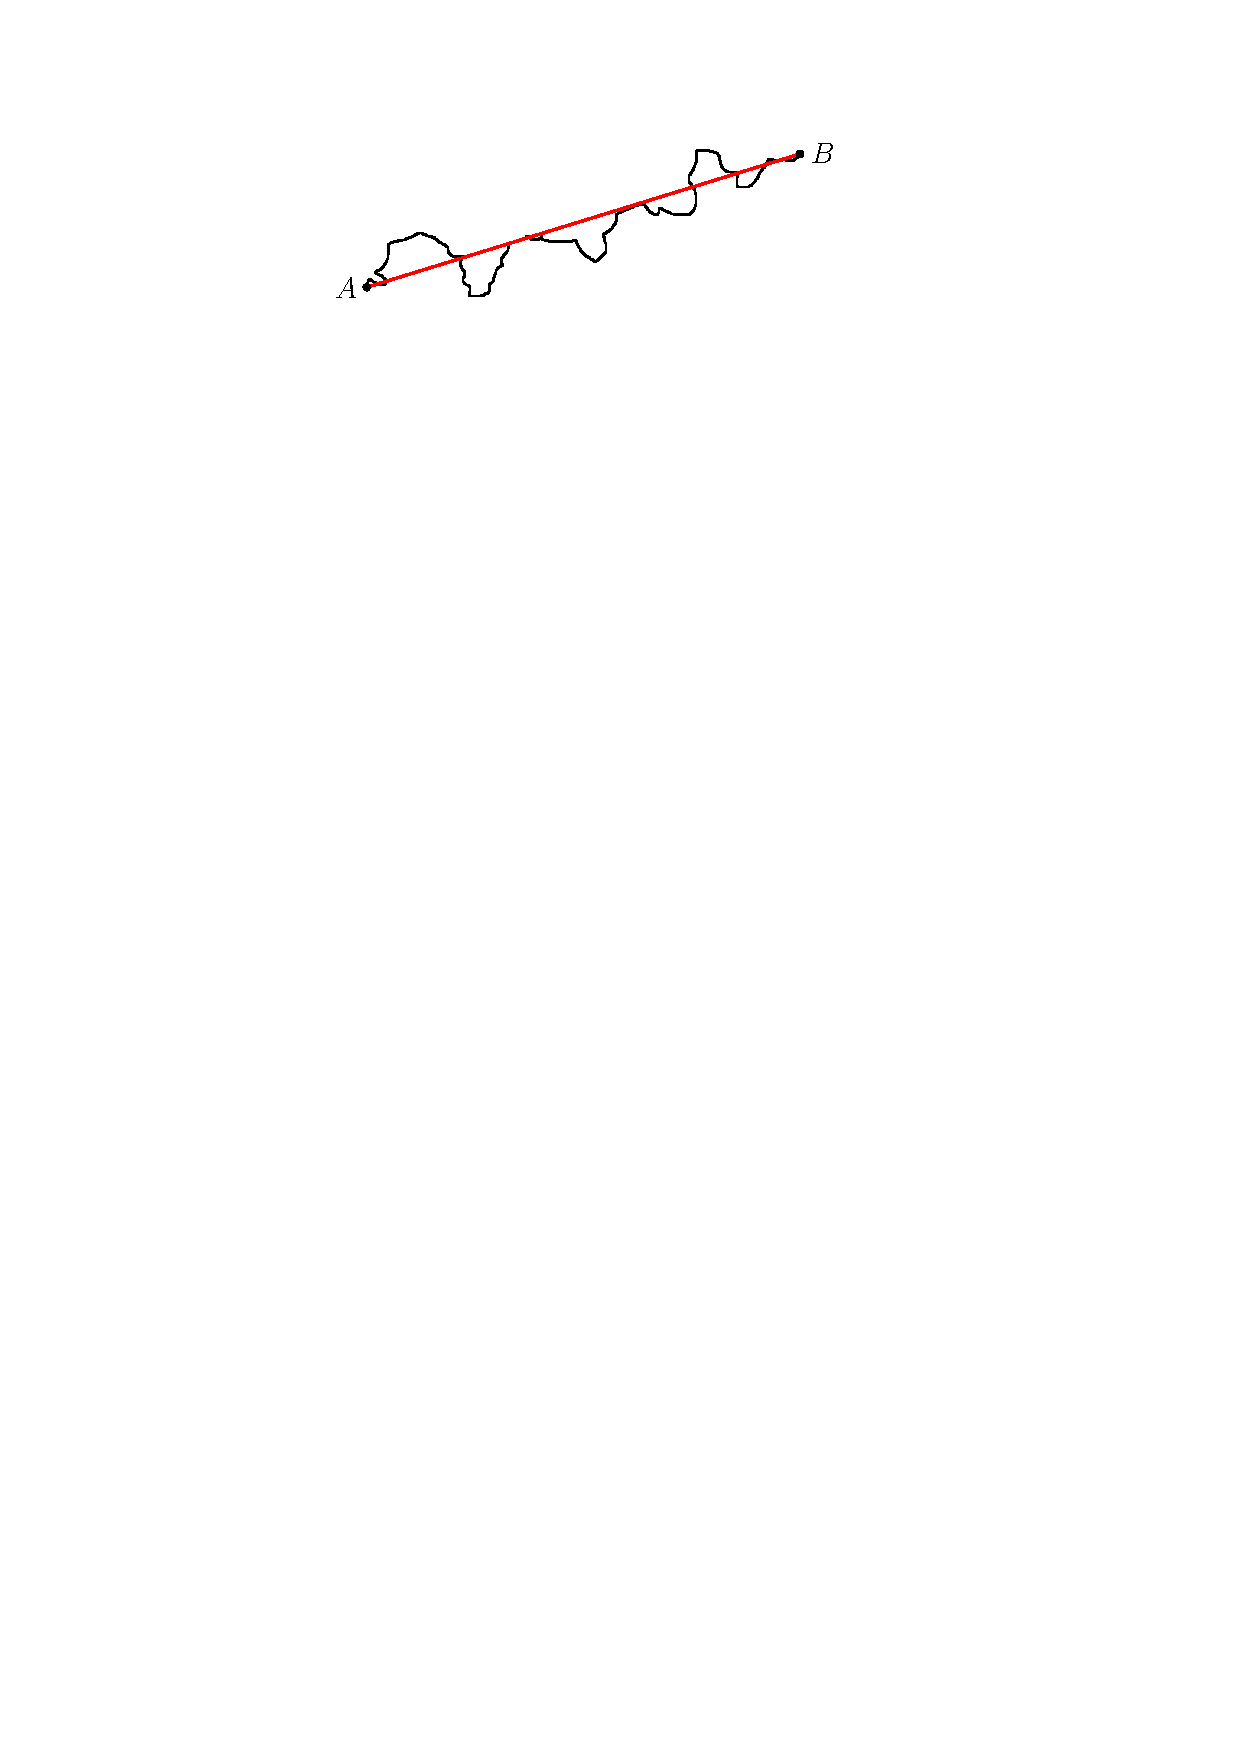
\includegraphics[scale=\normalipe]{ch01-pobrezi.pdf}
    \caption{Příklad mapy pobřeží se spojnicí bodů $A$ a~$B$.}
    \label{fig:pobrezi}
\end{figure}
Zjevně jeho délka je zdola omezena délkou spojnice koncových bodů $A$ a~$B$, nicméně typické pobřeží je velmi nepravidelné a~klikaté. Existují různé metody, které nám umožňují určit jeho délku přesněji. Několik z~nich je popsáno v~knize \citep[str. 79]{Mandelbrot1983}, pro uvedení do problematiky si zde však vystačíme s~tou nejednodušší.\par
Předpokládejme, že pobřeží, které zkoumáme, má pevné hranice (tj. zanedbáváme např. přílivy a~odlivy nastávající během dne), a dále jsme schopni rozlišovat libovolně krátké vzdálenosti.\par
Mějme zadané libovolné $\varepsilon>0$. Podél pobřeží začneme umisťovat tyče tak, že po každém umístění provedeme na mapě krok délky \textbf{nejvýše} $\varepsilon$, přičemž začínáme v~bodě $A$ a~postupujeme až k~bodu $B$ (popř. pokud měříme délku pobřeží ostrova, pokračujeme dokud se nevrátíme tam, kde jsme začali). Předpokládejme, že jsme provedli celkově $n(\varepsilon)$ kroků (jejich počet je závislý na zvolené délce kroku). \emph{Přibližnou délku pobřeží} $\ell(\varepsilon)$ pak stanovíme jako
\begin{equation*}
    \ell(\varepsilon)=n(\varepsilon)\cdot\varepsilon.
\end{equation*}
\begin{figure}[h]
    \centering
    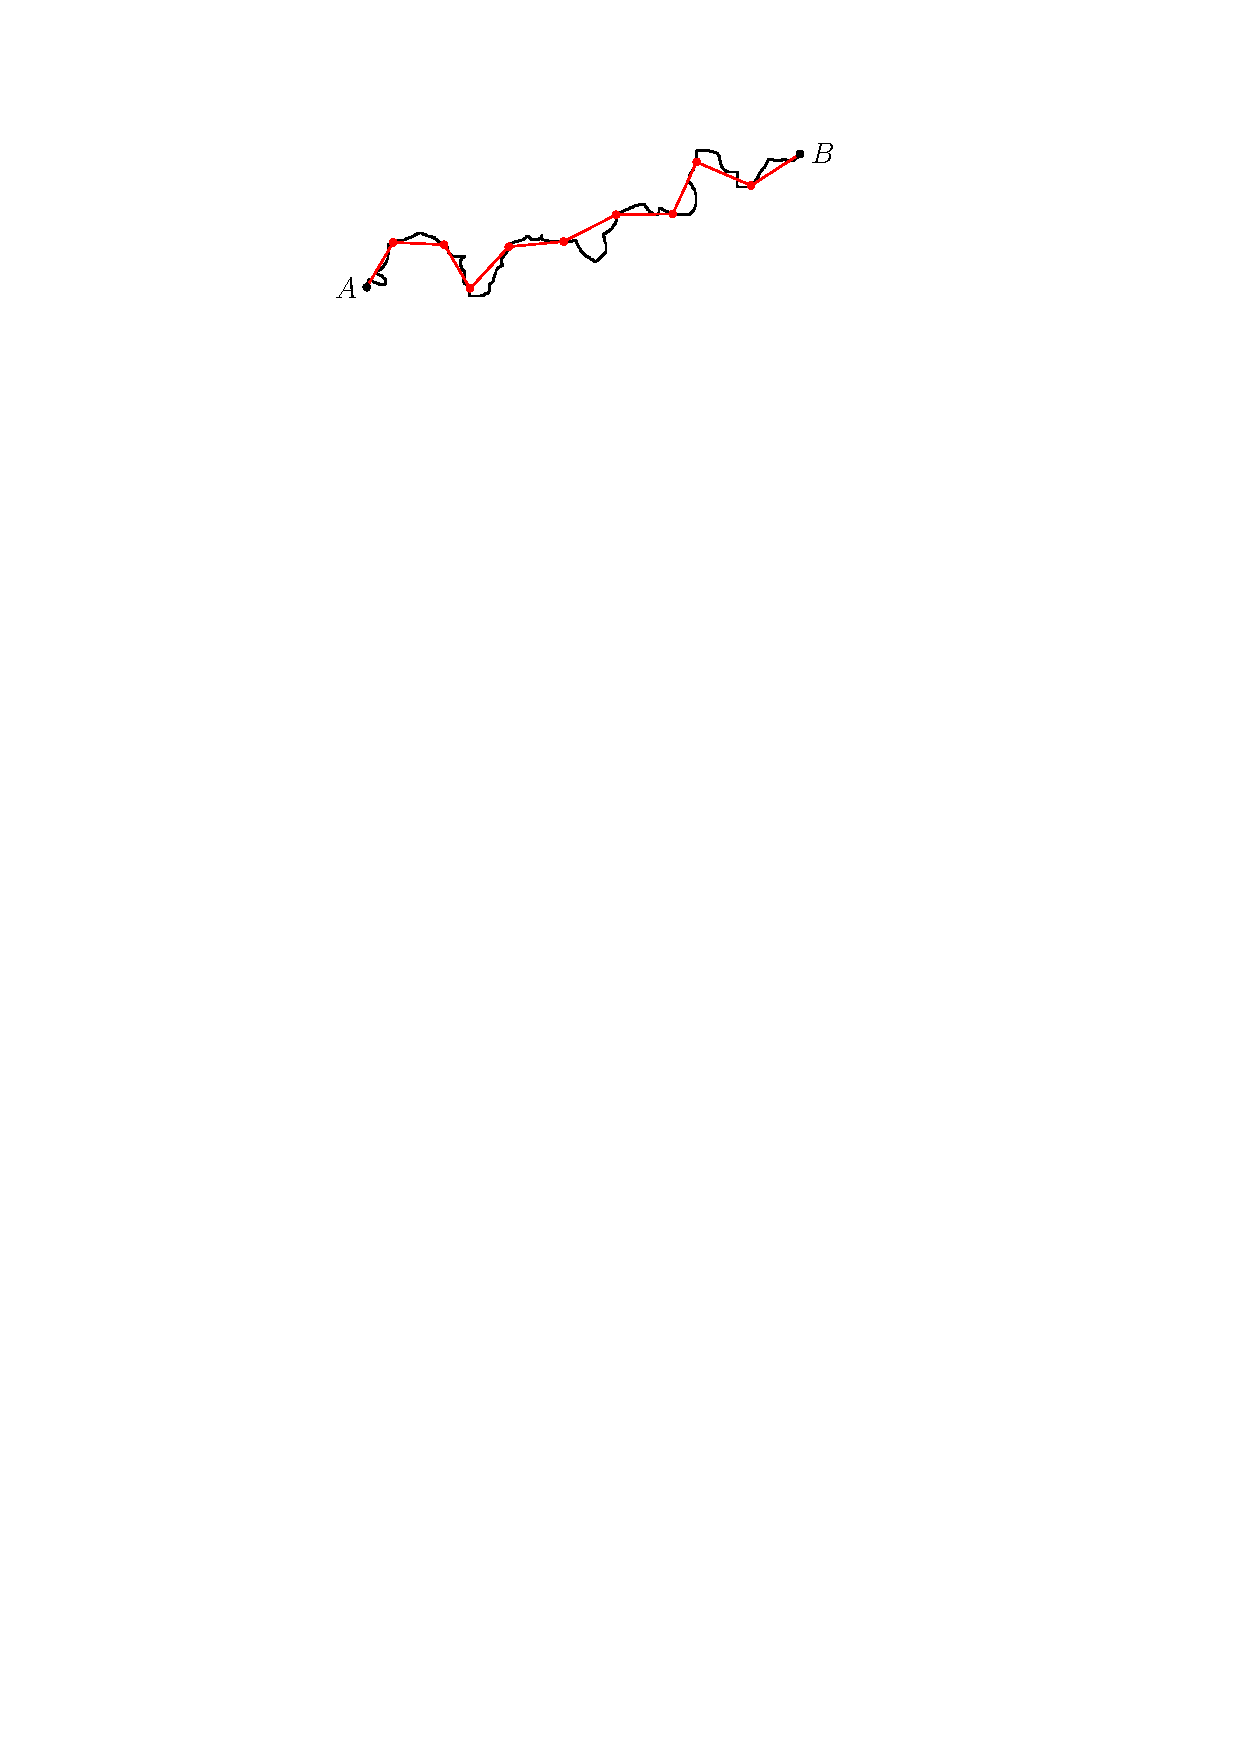
\includegraphics[scale=\normalipe]{ch01-pobrezi-aproximace.pdf}
    \caption{Odhad délky pobřeží, kde $n=10$ při zvoleném $\varepsilon$.}
    \label{fig:pobrezi_aproximace}
\end{figure}
Nyní by nás mohlo napadnout, že pro zmenšující se $\varepsilon$, tj. $\varepsilon\to0_+$, bude hodnota $\ell(\varepsilon)$ konvergovat ke skutečné délce pobřeží. Tzn.~označíme-li skutečnou délku pobřeží $L$, pak bychom mohli očekávat, že platí
\begin{equation}\label{eq:aproximace_limita}
    L=\lim_{\varepsilon\to0_+}{\ell(\varepsilon)}.
\end{equation}
Jenže, bohužel, limita \eqref{eq:aproximace_limita} bude v reálné situaci rovna $\infty$. Proč? Je třeba si uvědomit, že zde pracujeme s~\emph{mapou} pobřeží, která má určité \emph{měřítko}. Pokud bychom měli pobřeží na mapě s~měřítkem $1\,:\,100\;000$, uvidíme méně detailů, než kdybychom jej zkoumali na mapě s~měřítkem $1\,:\,1\;000$. (Viz obrázek~\ref{fig:pobrezi_zoom}.)\par
\begin{figure}[h]
    \centering
    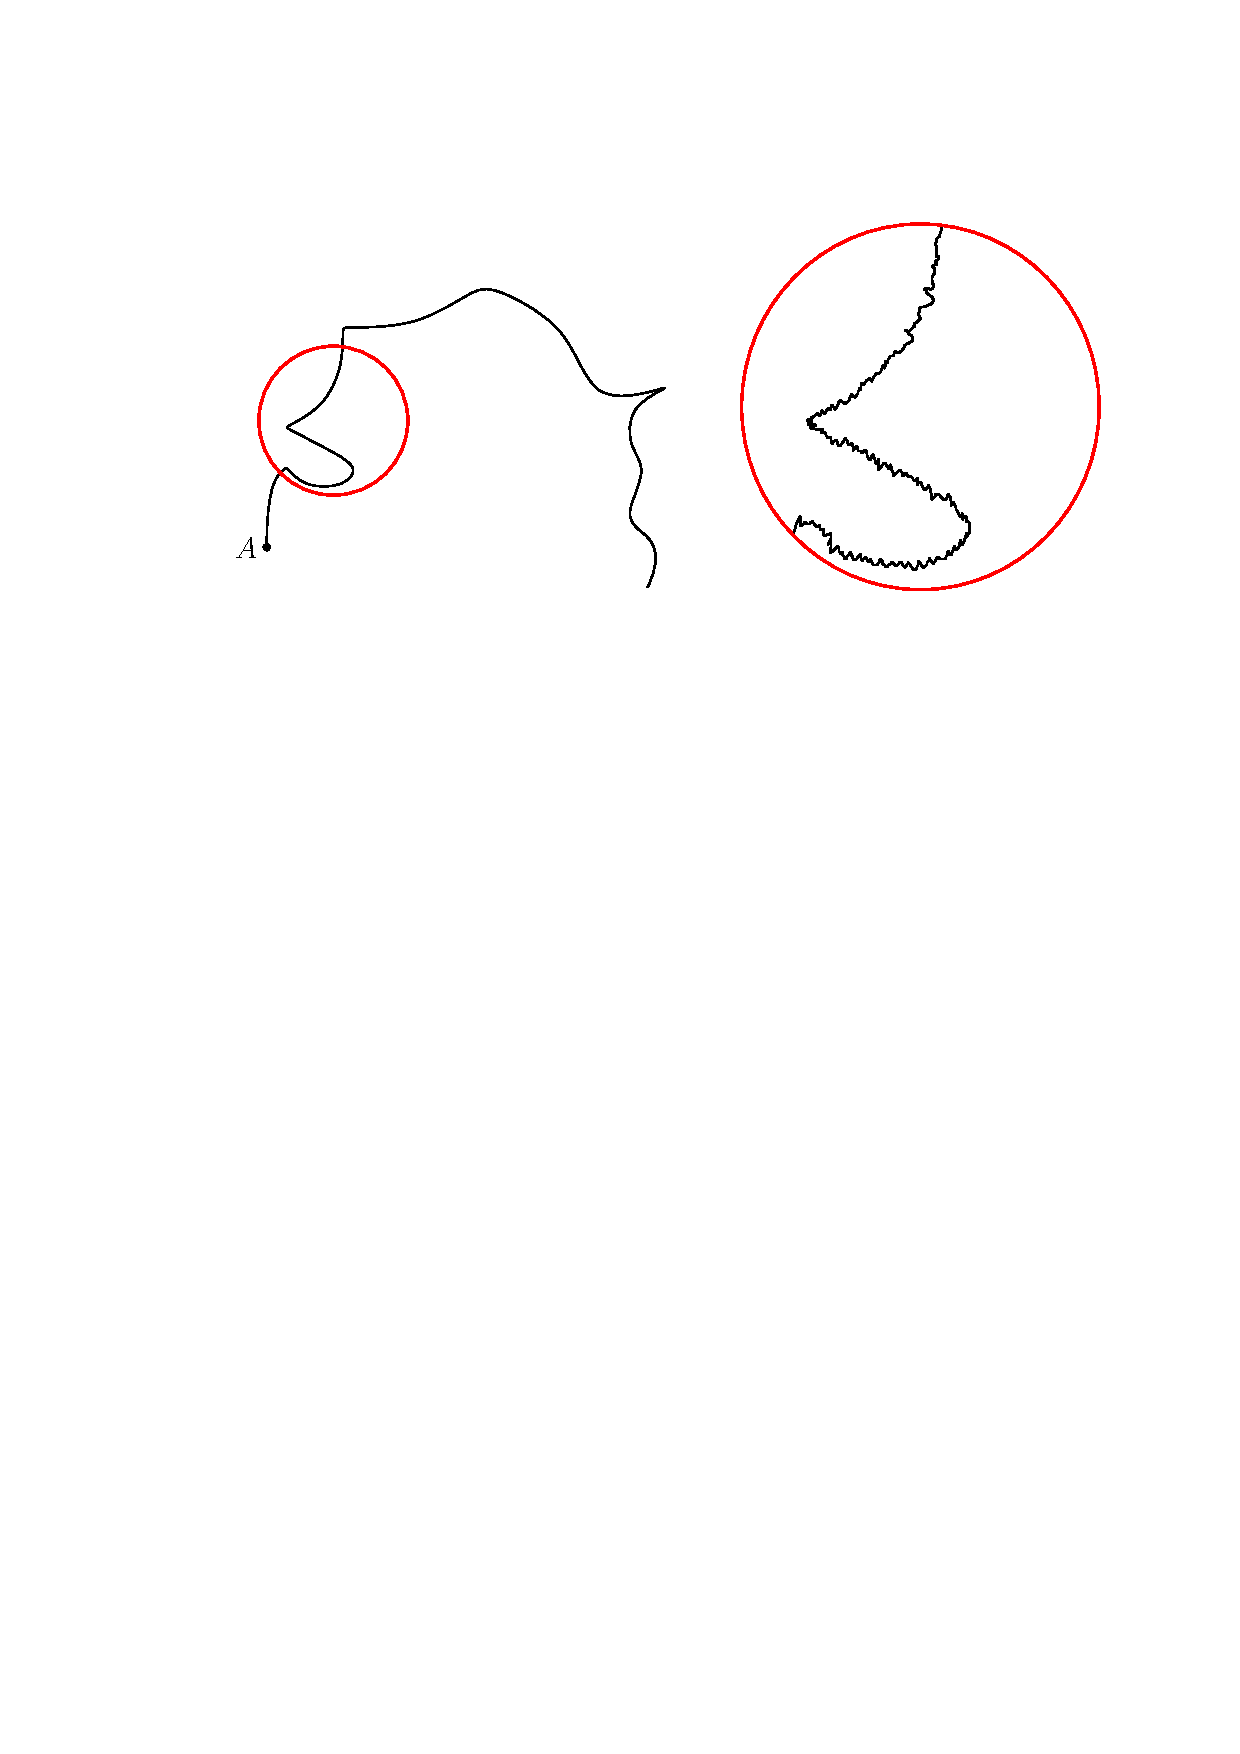
\includegraphics[scale=\normalipe]{ch01-pobrezi-zoom.pdf}
    \caption{Část pobřeží od bodu $A$ v~menším měřítku.}
    \label{fig:pobrezi_zoom}
\end{figure}
Nově odhalené detaily (menší poloostrůvky apod.) zde přispívají k~celkové délce pobřeží $\ell(\varepsilon)$. Postupným zvětšováním měřítka mapy bychom tak odhalili další detaily. Naše původní idea tak selhává, neboť (v "klasickém" pojetí délky) pro $\varepsilon\to0_+$ hodnota $\ell(\varepsilon)$ patrně poroste nade všechny meze, tj. $\lim_{\varepsilon\to0_+}{\ell(\varepsilon)}=\infty$.\par
Nabízí se otázka: Proč se toto děje? Pokud se ohlédneme zpět za eukleidovskou geometrií\index{geometrie!eukleidovská}\index{eukleidovská geometrie}, tento problém v ní nenastává. Např. u~kružnice v~eukleidovské rovině $\mathbb{E}_2$ změnou měřítka žádné další detaily křivky neobjevíme (podobně u~jiných geometrických útvarů, viz obrázky~\ref{subfig:kruznice} a~\ref{subfig:kruznice_zoom}). 
\begin{figure}[h]
    \centering
    \begin{subfigure}{\subfigwidth}
        \centering
        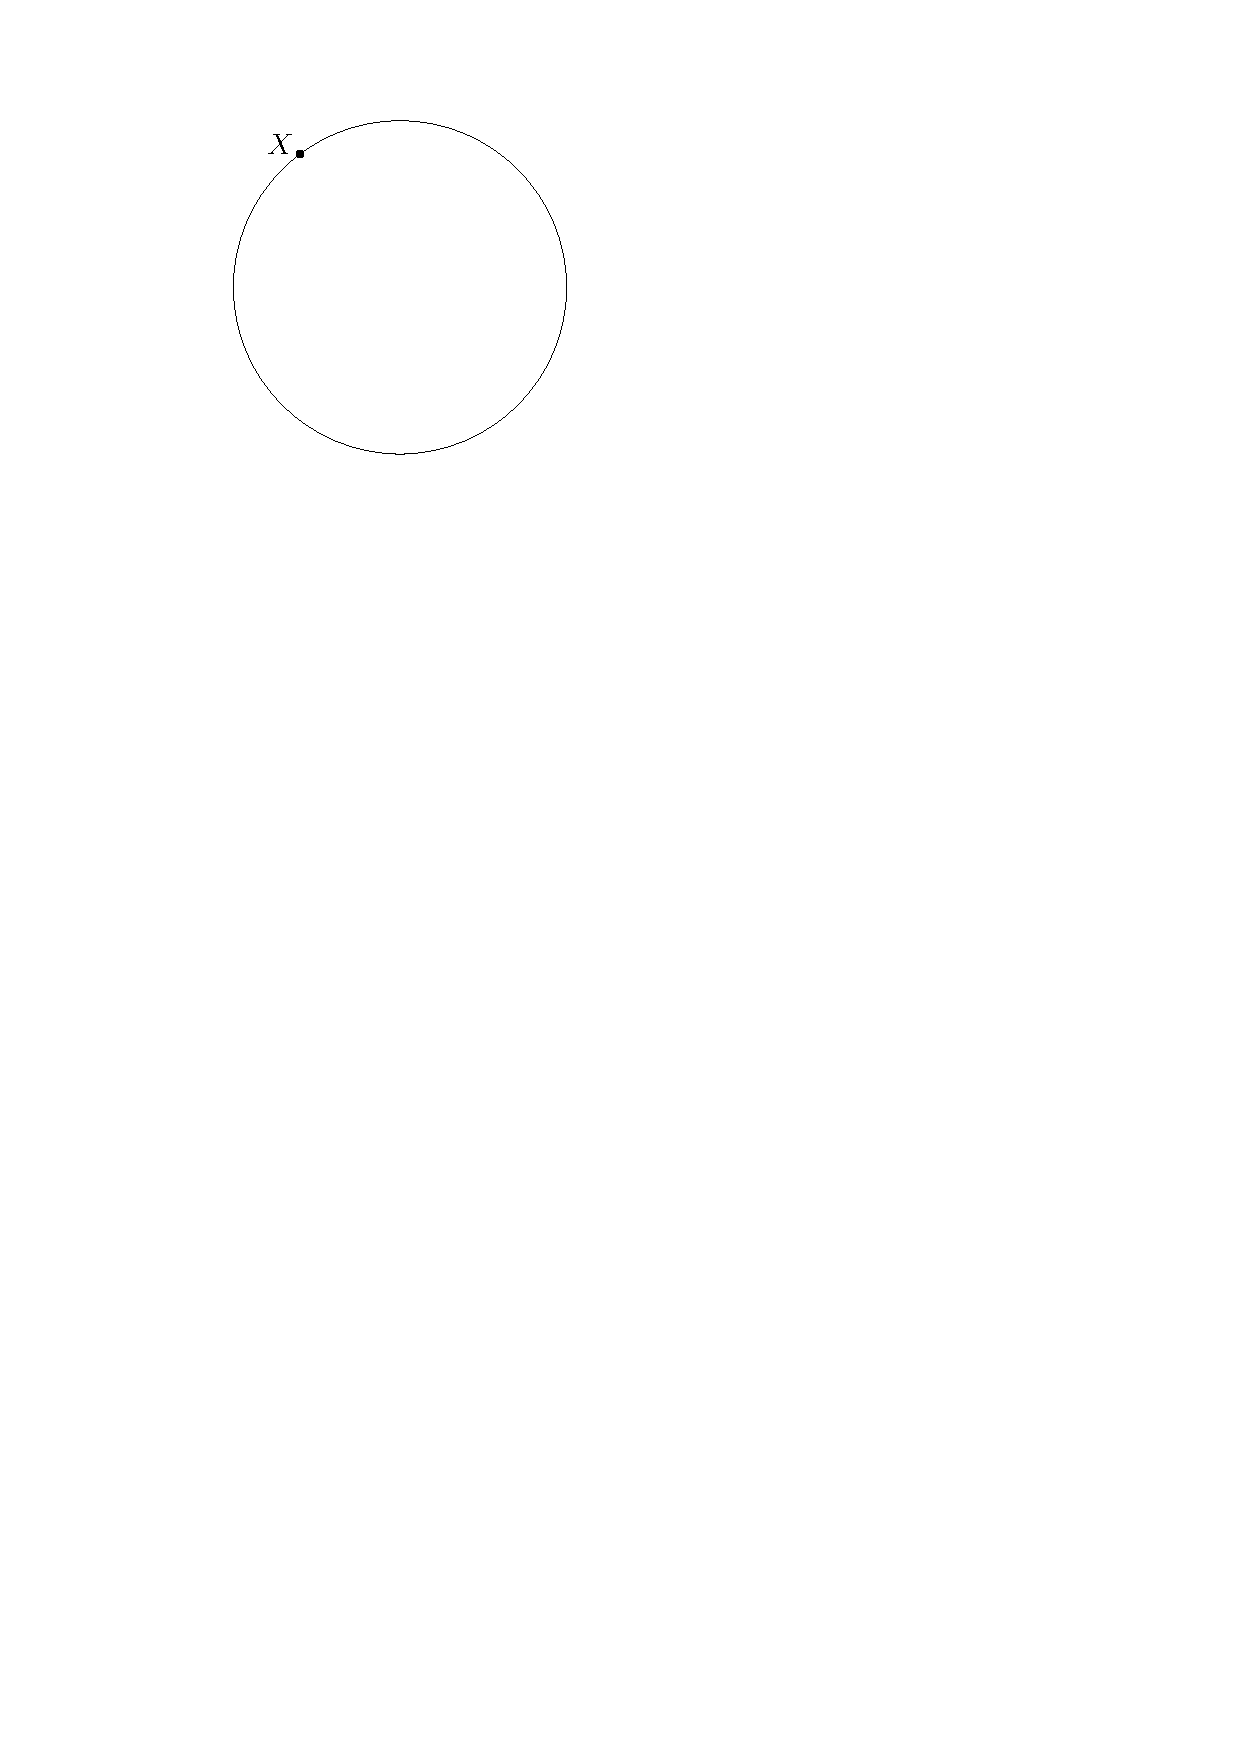
\includegraphics[scale=\normalipe]{ch01-kruznice.pdf}
        \caption{Kružnice v~menším měřítku.}
        \label{subfig:kruznice}
    \end{subfigure}
    \quad
    \begin{subfigure}{\subfigwidth}
        \centering
        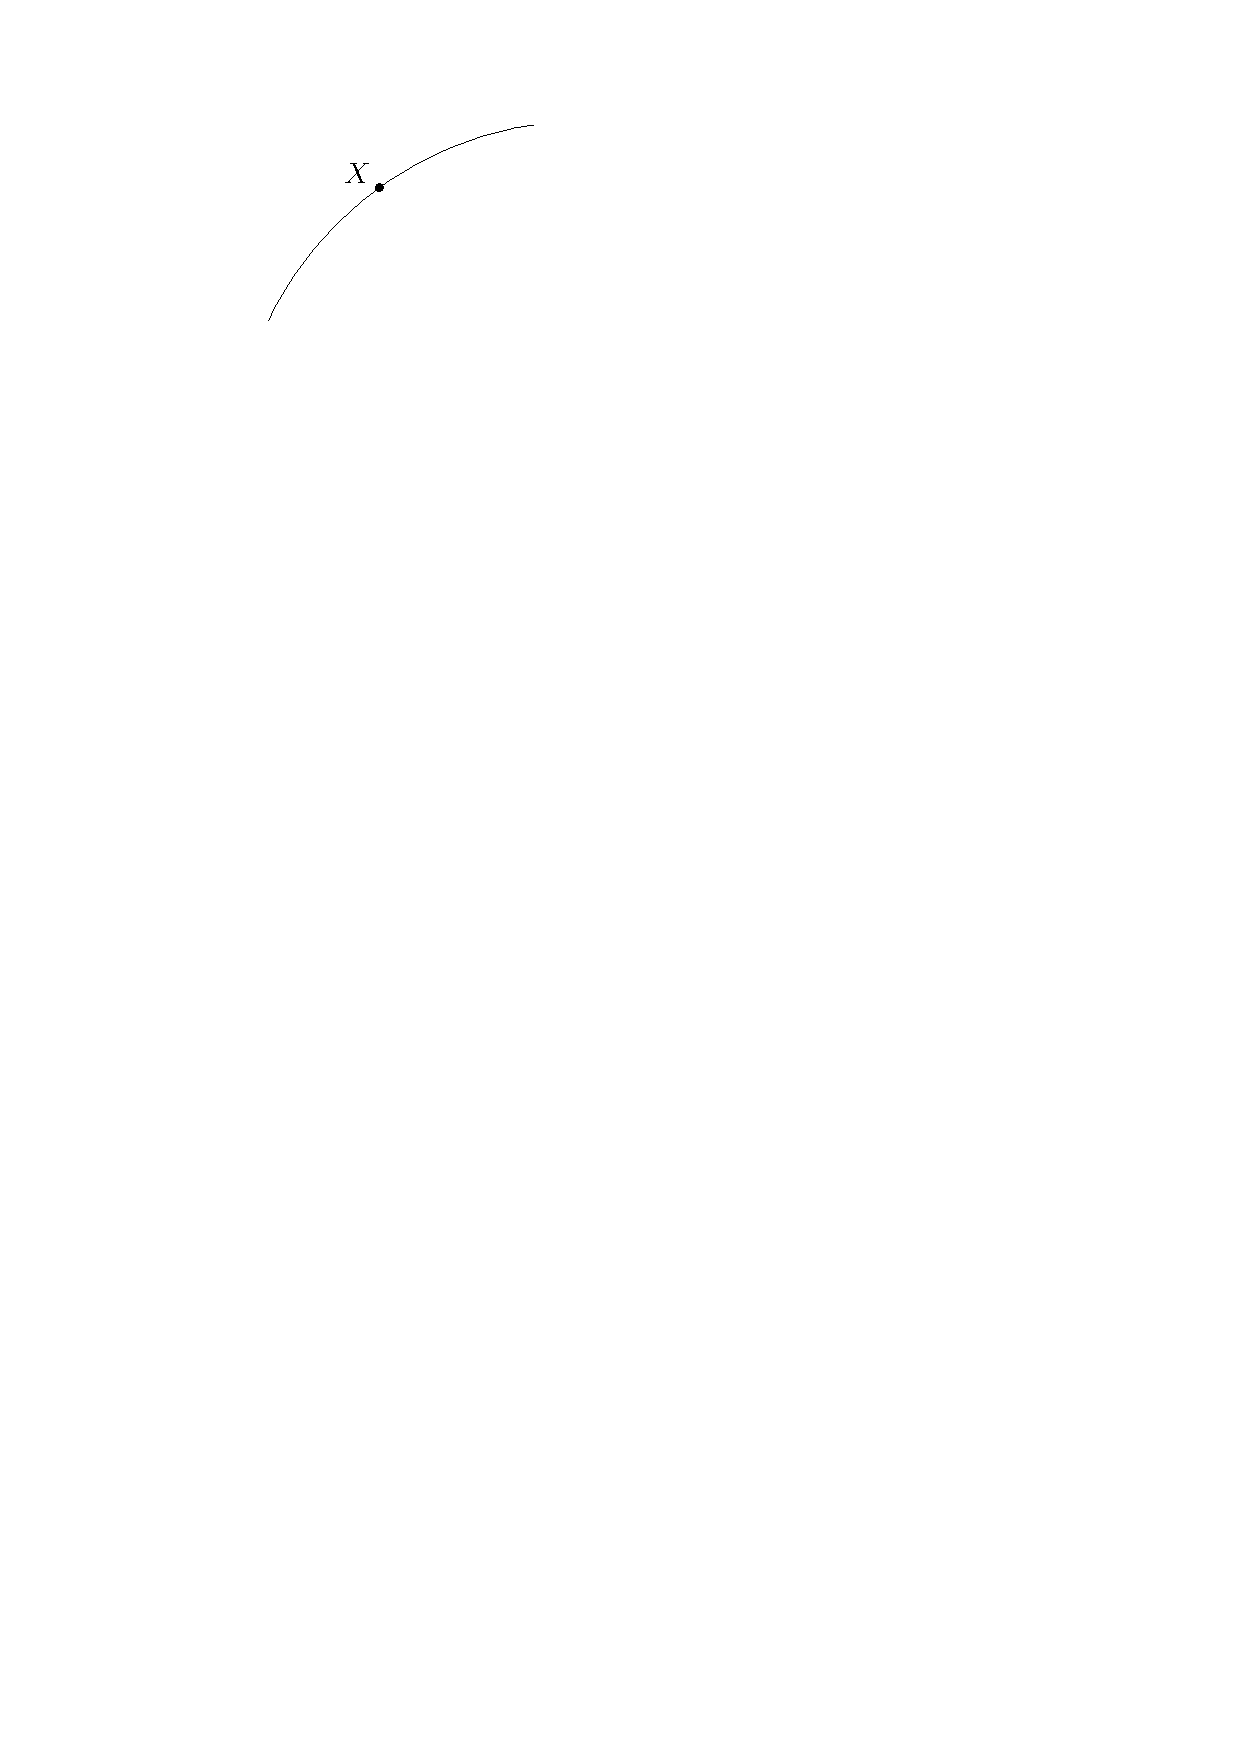
\includegraphics[scale=\normalipe]{ch01-kruznice-zoom.pdf}
        \caption{Část kružnice ve větším měřítku.}
        \label{subfig:kruznice_zoom}
    \end{subfigure}
\end{figure}
Díky tomu můžeme v~případě počítání obvodu kružnice použít následující postup.\par
Máme-li kružnici o~poloměru $r>0$, pak jí můžeme vepsat libovolný pravidelný $n$-úhelník (viz obrázek~\ref{subfig:archimedova_metoda}).
\begin{figure}[h]
    \centering
    \begin{subfigure}{\subfigwidth}
        \centering
        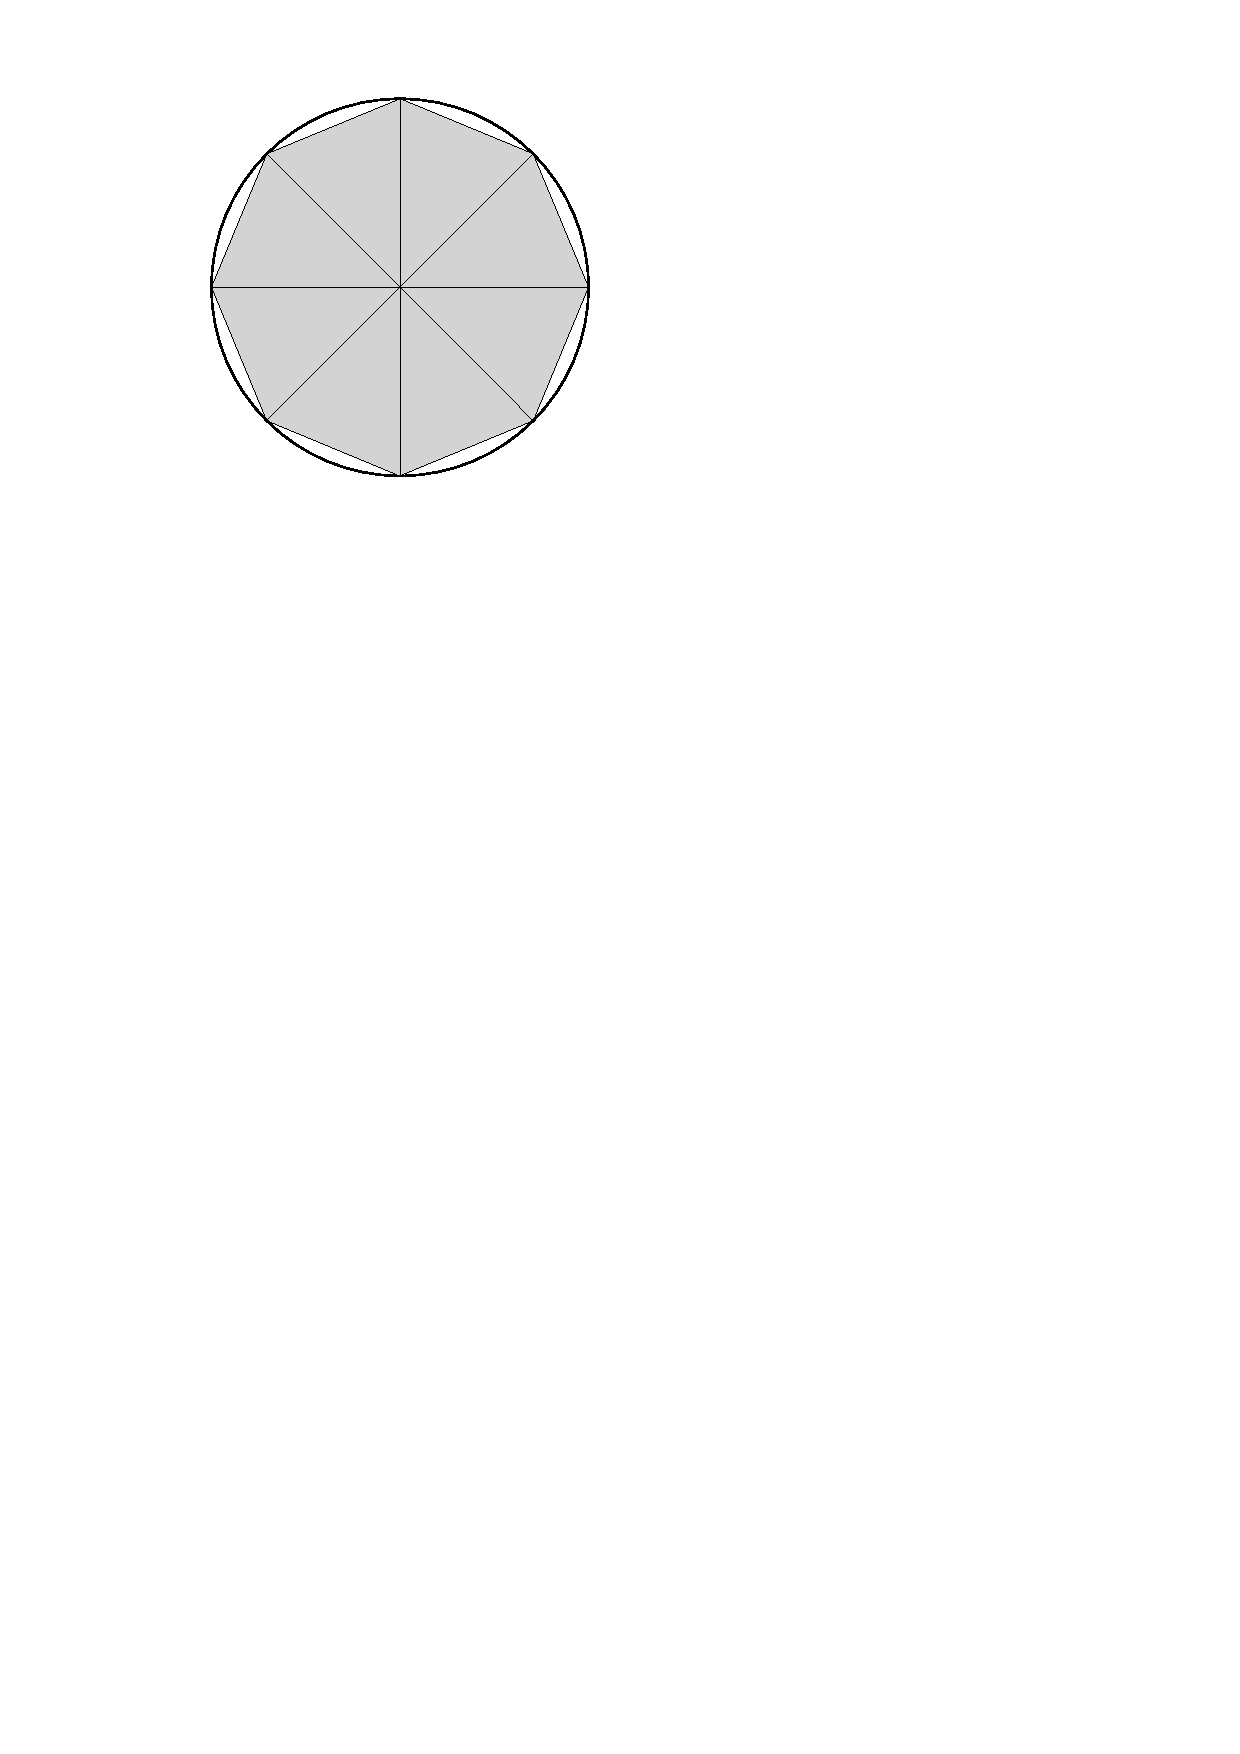
\includegraphics[scale=\normalipe]{ch01-archimedova-metoda.pdf}
        \caption{Pravidelný osmiúhelník vepsaný kružnici.}
        \label{subfig:archimedova_metoda}
    \end{subfigure}
    \quad
    \begin{subfigure}{\subfigwidth}
        \centering
        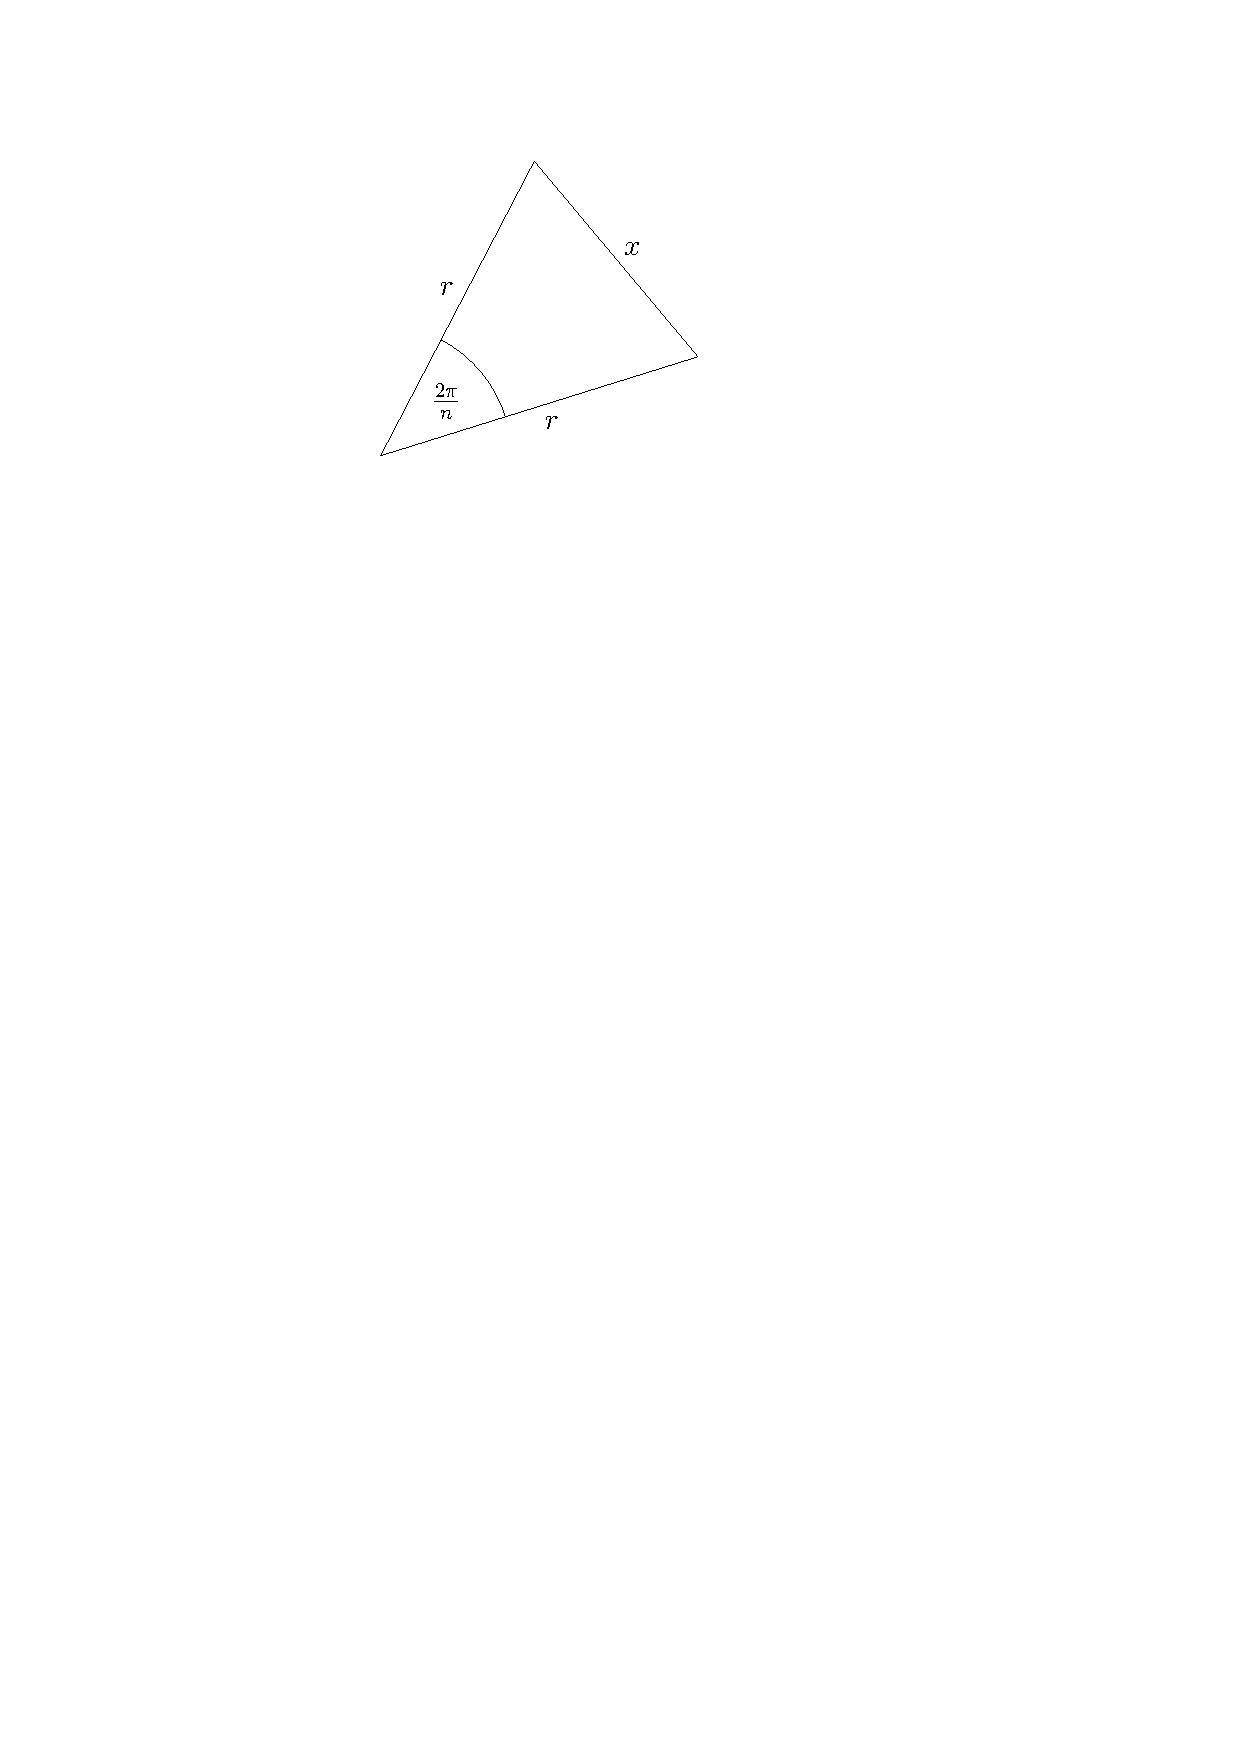
\includegraphics[scale=\normalipe]{ch01-archimedova-metoda-cast-nuhelniku.pdf}
        \caption{Část vepsaného pravidelného $n$-úhelníku.}
        \label{subfig:archimedova_metoda_cast_nuhelniku}
    \end{subfigure}
    \caption{Princip Archimédovy metody.}
    \label{fig:princip_archimedovy_metody}
\end{figure}
Obvod pravidelného $n$-úhelníku is označíme $O_n$ a~délku jeho strany $x$ (viz obrázek~\ref{subfig:archimedova_metoda_cast_nuhelniku}). Tu jsme schopni stanovit užitím elementární goniometrie, tj.
\begin{equation*}
    x=2r\cdot\sin{\dfrac{\pi}{n}},
\end{equation*}
a tedy obvod
\begin{equation*}
    O_n=2rn\cdot\sin{\dfrac{\pi}{n}}.
\end{equation*}
Pro rostoucí $n$ bude obvod pravidelného $n$-úhelníku stále lépe aproximovat obvod původní kružnice (viz obrázek~\ref{fig:archimedova_metoda_presnejsi}).
\begin{figure}[h]
    \centering
    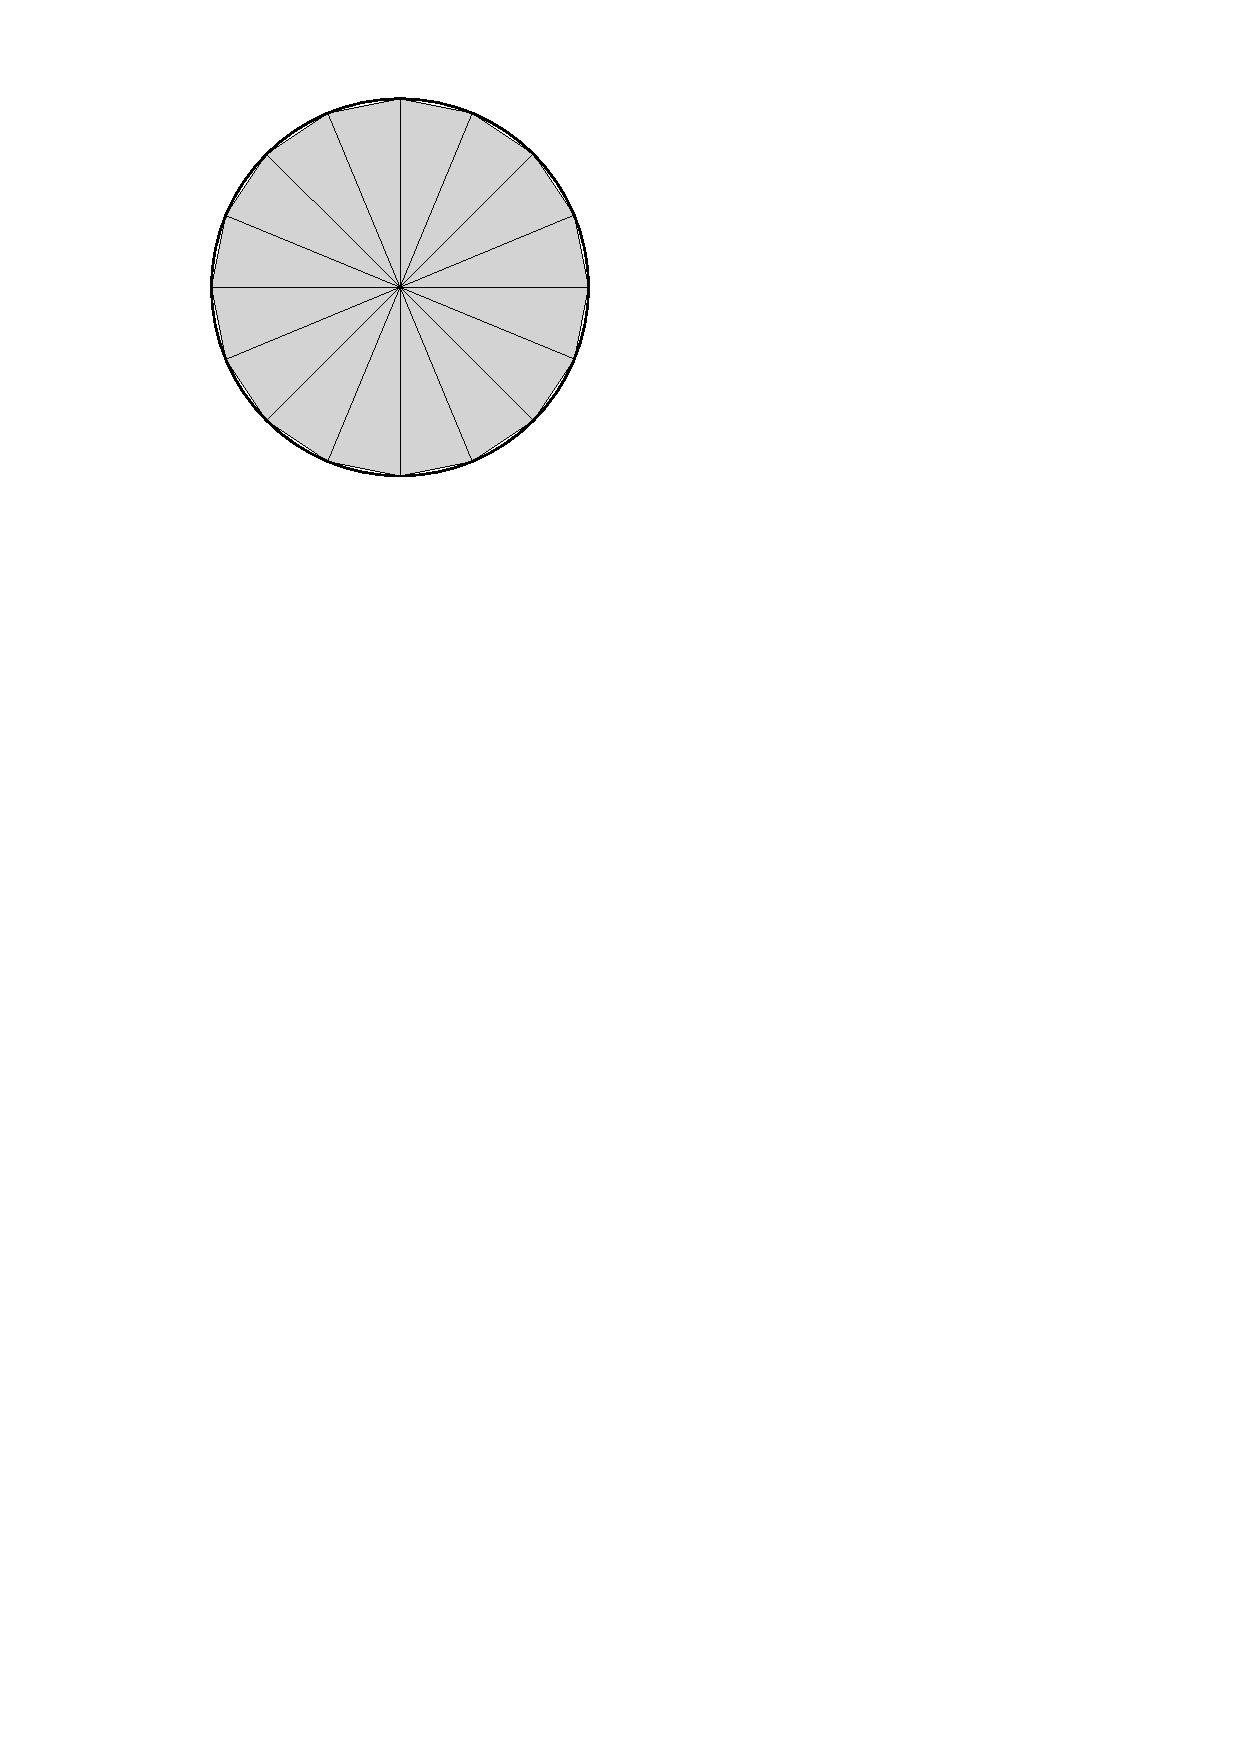
\includegraphics[scale=\normalipe]{ch01-pobrezi-aproximace-presnejsi.pdf}
    \caption{Aproximace obvodu kružnice pomocí pravidelného šestnáctiúhelníku.}
    \label{fig:archimedova_metoda_presnejsi}
\end{figure}
Limitním přechodem (tj. pro $n\to\infty$) tak můžeme odvodit vzorec pro obvod kružnice:
\begin{align*}
    O&=\lim_{n\to\infty}{2rn\cdot\sin{\dfrac{\pi}{n}}}=2r\cdot\lim_{n\to\infty}{n\cdot\sin{\dfrac{\pi}{n}}}=2\pi r\cdot\lim_{n\to\infty}{\cdot\dfrac{\sin{\dfrac{\pi}{n}}}{\dfrac{\pi}{n}}}=2\pi r.
\end{align*}
Idea aproximace pomocí "zjemňování" zde skutečně funguje a~délka ve standardním pojetí tak dává smysl, jak bychom mohli očekávat. Křivka, kterou tvoří pobřeží, má však oproti kružnici jiný geometrický charakter. Délka pobřeží $\infty$, k~níž Mandelbrot došel, tak dává smysl \emph{z geometrického pohledu}, avšak výsledek to není moc užitečný.
\section{Soběpodobnost}\label{sec:sobepodobnost}
Mandelbrot si uvědomil,~že struktura pobřeží se charakterově vymyká útvarům do tehdy známým eukleidovské geometrii,~neboť mapy s~různými měřítky poskytovaly různou úroveň detailů,~které hrály netriviální roli v~jeho celkové délce. Učinil však jiné zásadní pozorování,~a to sice,~že mnoho detailů má společné rysy,~které se opakují. Hodně z~nich se shodovalo s~výjimkou jejich měřítka. \citep[str. 96]{Mandelbrot1983}\par

Ve fraktální geometrii se pro tento úkaz uchytil termín \emph{soběpodobnost} (angl. \emph{self-similarity}). Útvar nazýváme soběpodobným,~\textbf{pokud se sám sobě podobný v~libovolném měřítku} \citep[str. 220]{Voracova2022} nebo pokud \textbf{část útvaru je podobná jeho celku}. Zmíněná podoba může být míněna přibližně (např. v~případě pobřeží je nejspíše jasné,~že žádné z~jeho detailů nesdílejí společné rysy přesně),~ale v~dalších částech si předvedeme soběpodobnost \emph{přímou}\index{soběpodobnost}.

\subsection{Kochova křivka}\label{subsec:kochova_krivka}
Jak jsme si již uvedli,~za otce fraktální geometrie je považován Mandelbrot,~avšak mnoho fraktálních křivek bylo známo již dříve (čtenář promine,~že jsme blíže nespecifikovali termín "fraktální",~jeho přesný význam pro nás však zatím nebude stěžejní). Jako první se podíváme na jednu z~nejznámějších,~kterou objevil roku \emph{1904} švédský matematik \name{Helge~von~Koch} \mbox{(1870--1924)},~dnes známou pod~názvem \emph{Kochova křivka}\index{Kochova křivka}\index{křivka!Kochova}. \citep[str. 61]{Peitgen2004} Na začátku vezmeme úsečku délky $1$. Vyjmeme prostřední (tj. druhou) třetinu a nahradíme ji dvěma úsečkami délky $1/3$,~tak,~aby na sebe navazovaly v~krajních bodech. Tento proces následně opakujeme pro nově vzniklé úsečky. Obecně u~úsečky délky $l$ nahradíme její prostřední třetinu dvojicí úseček délek $l/3$ (viz obrázek \ref{fig:kochova_vlocka_5iteraci}).
\begin{figure}[h]
    \centering
    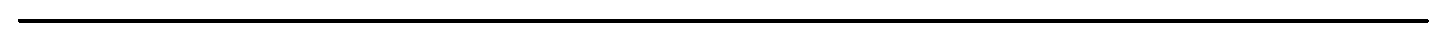
\includegraphics[scale=\fractalscale]{ch01-kochova-krivka-0iterace.pdf}\\\qquad\\
    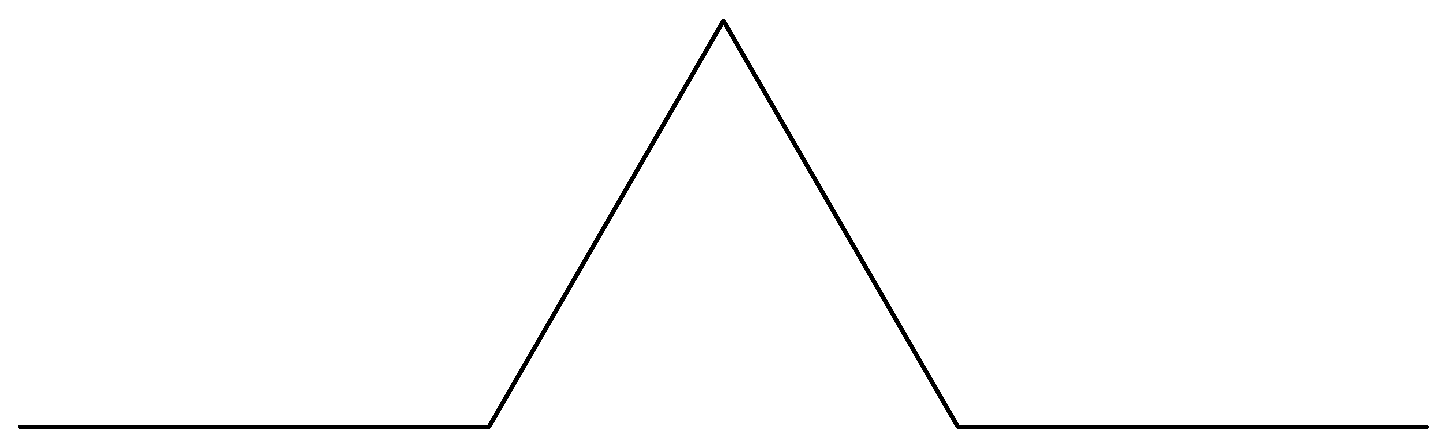
\includegraphics[scale=\fractalscale]{ch01-kochova-krivka-1iterace.pdf}\\\qquad\\
    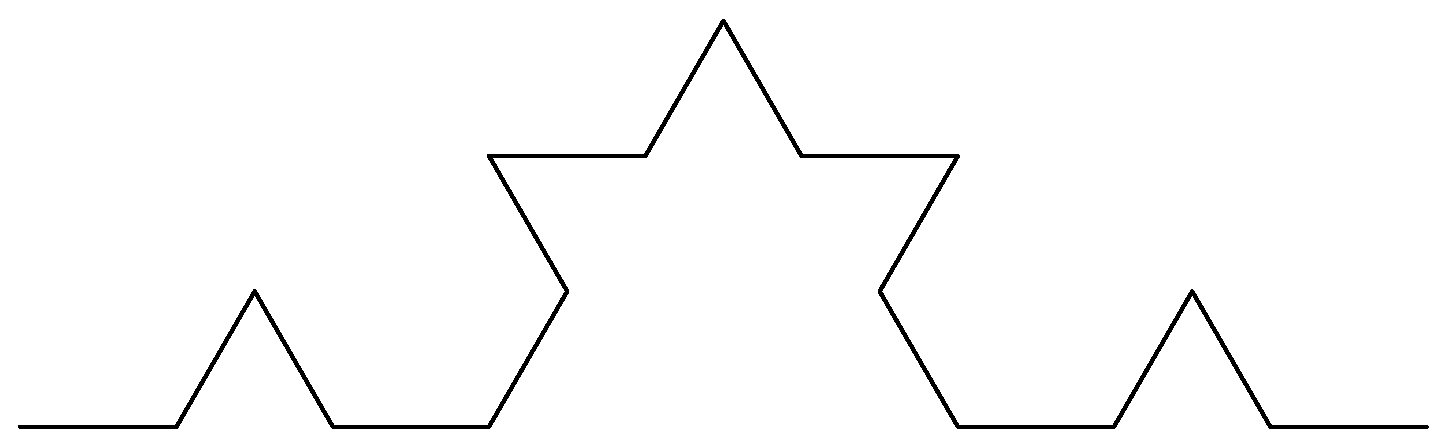
\includegraphics[scale=\fractalscale]{ch01-kochova-krivka-2iterace.pdf}\\\qquad\\
    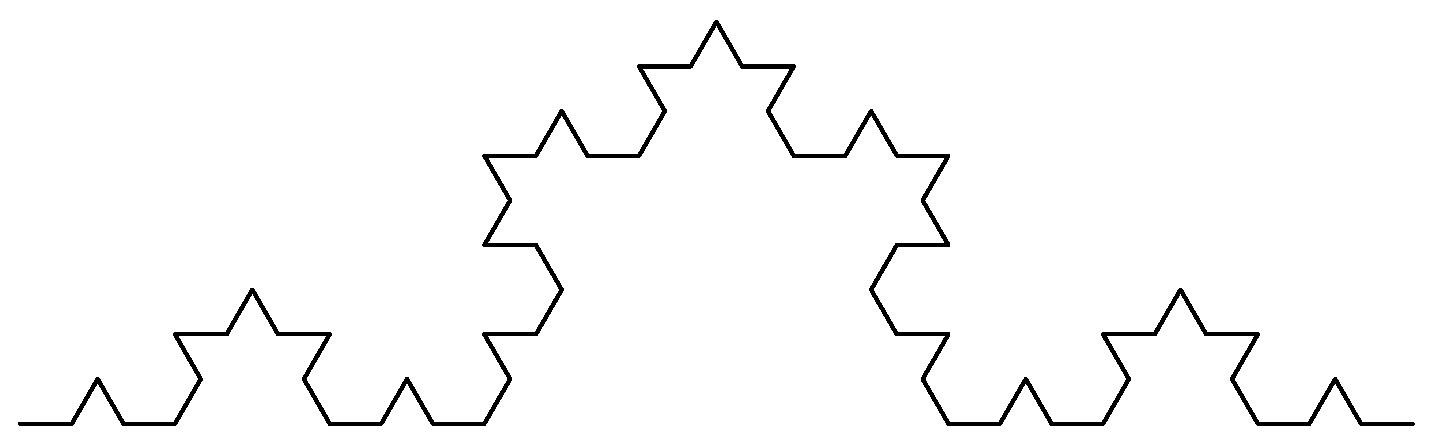
\includegraphics[scale=\fractalscale]{ch01-kochova-krivka-3iterace.pdf}\\\qquad\\
    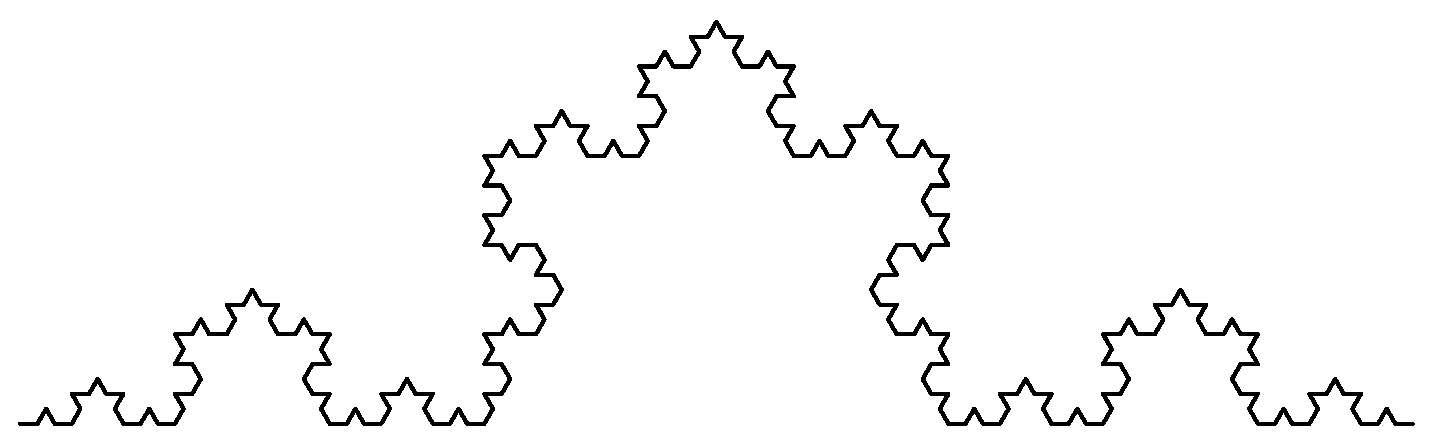
\includegraphics[scale=\fractalscale]{ch01-kochova-krivka-4iterace.pdf}\\\qquad\\
    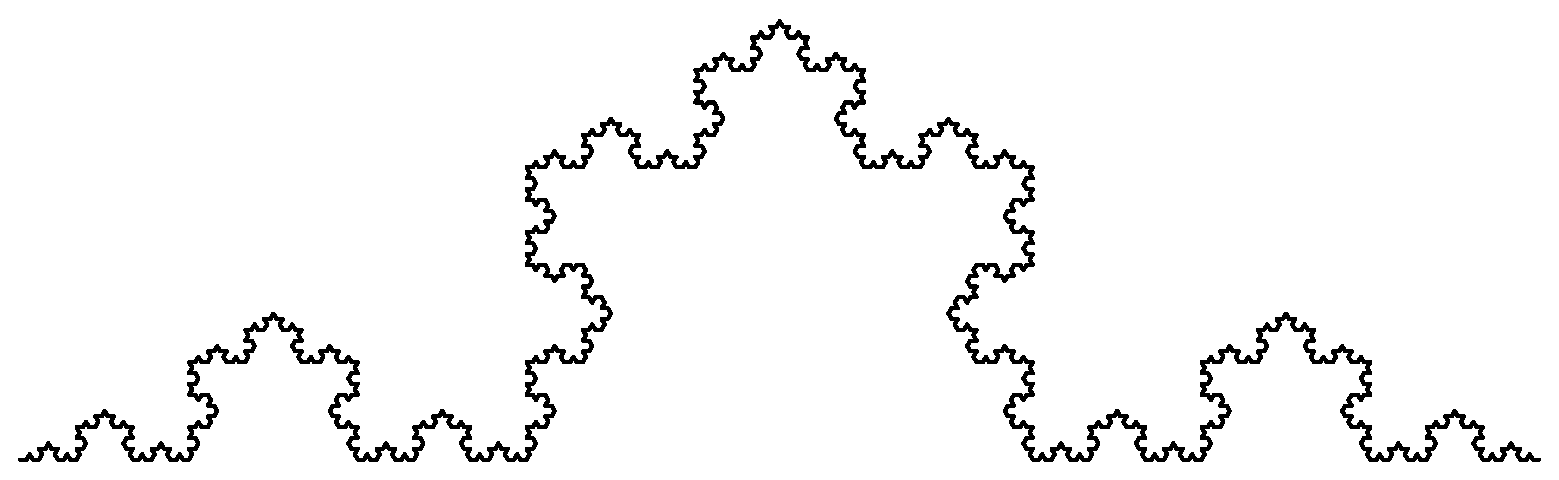
\includegraphics[scale=\fractalscale]{ch01-kochova-krivka-5iterace.pdf}
    \caption{Prvních pět iterací Kochovy křivky.}
    \label{fig:kochova_vlocka_5iteraci}
\end{figure}
V první řadě si můžeme všimnout,~že v~každé další iteraci jsou nově vzniklé podobné původnímu celku,~tedy v~předešlé iteraci (viz obrázek \ref{fig:kochova_krivka_podobnost}). Pokud by tento proces pokračoval do nekonečna,~pak by každá ze čtyř částí křivky představovala \textbf{celý původní obrazec} ve zmenšeném měřítku (byla by tedy soběpodobná).
\begin{figure}[h]
    \centering
    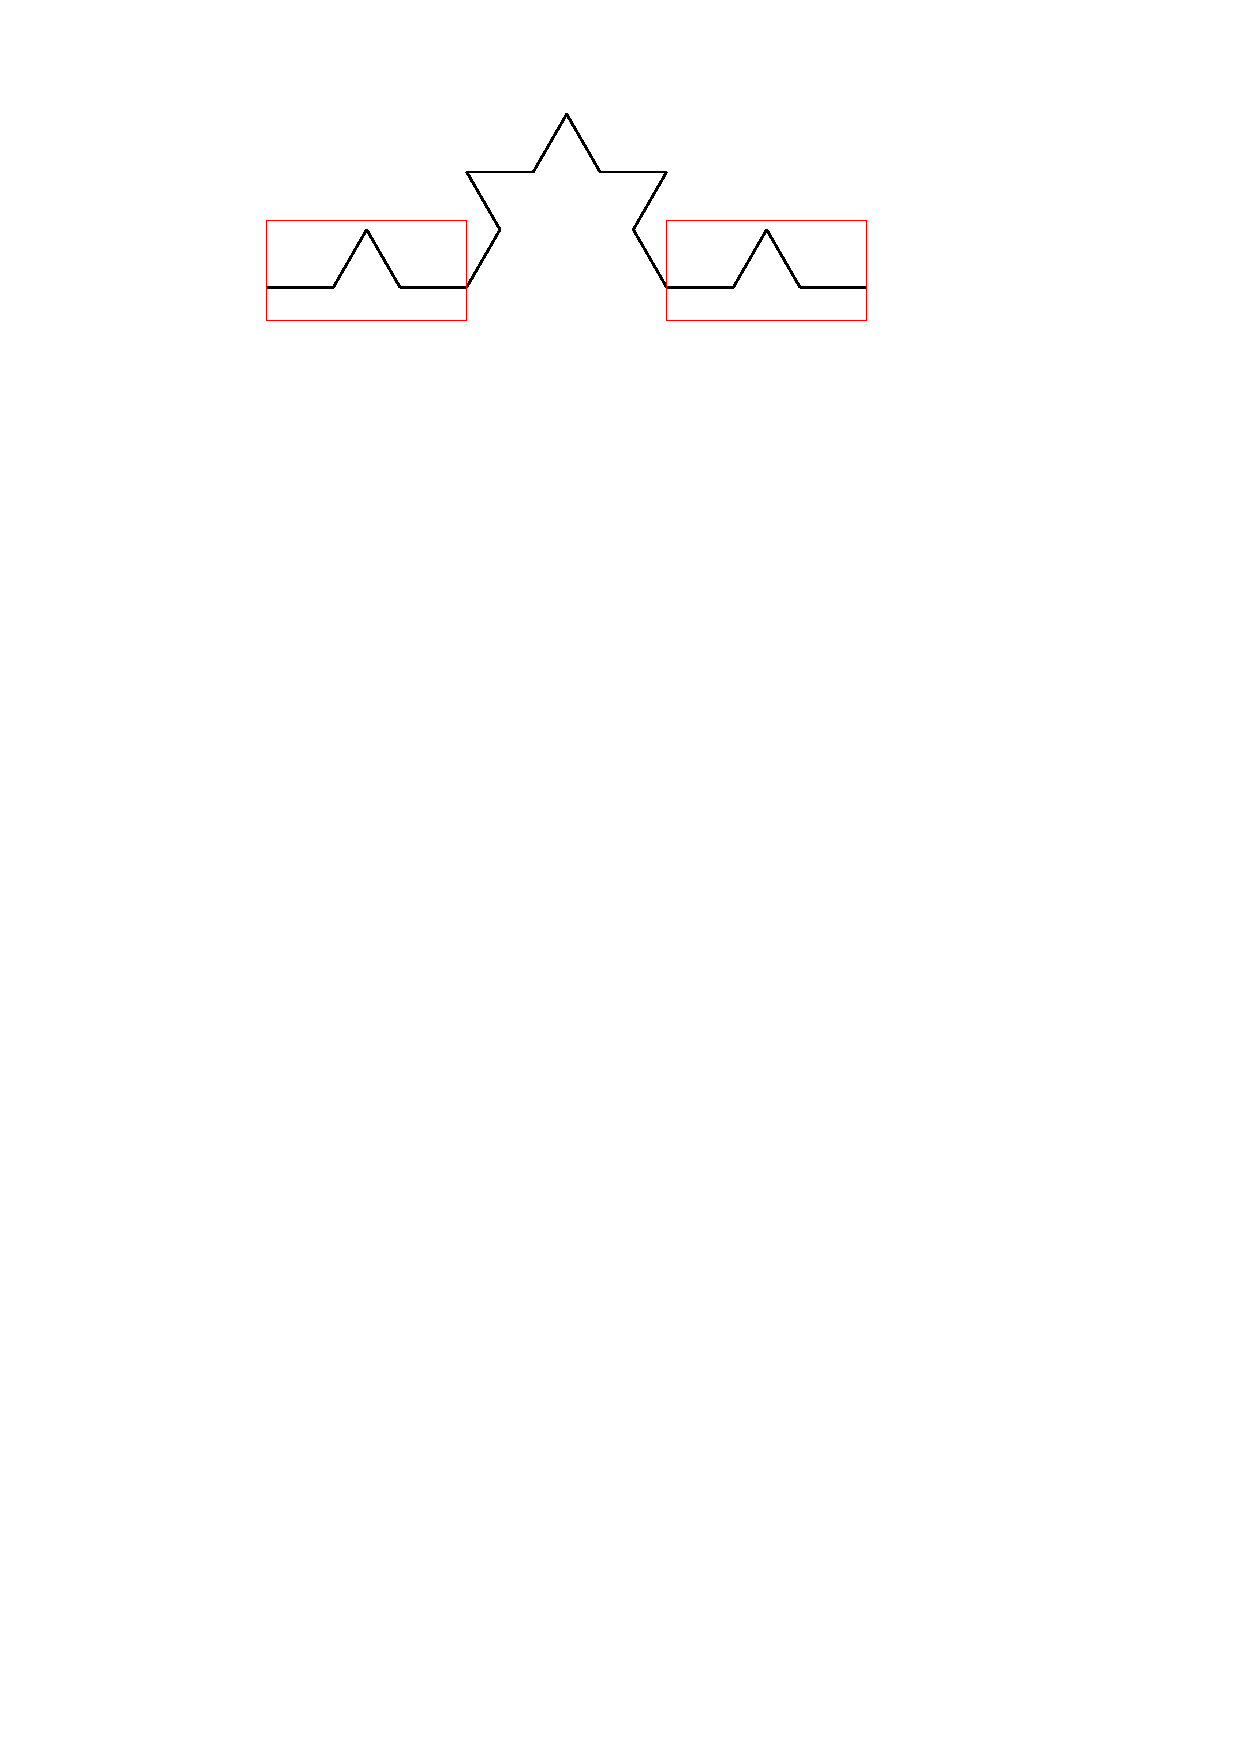
\includegraphics[scale=\normalipe]{ch01-kochova-krivka-podobnost.pdf}
    \caption{První iterace Kochovy křivky "uvnitř" druhé v~menším měřítku.}
    \label{fig:kochova_krivka_podobnost}
\end{figure}
Zkusme se nyní podívat na délku křivky. V~první iteraci začínáme s~úsečkou délky\footnote{Mohli bychom také začít s~obecnou délkou $\ell_0$,~ale ta by se však při výpočtu projevila pouze jako konstantní násobek.} $1$,~která se v~druhé iteraci změní na křivku délky $4/3$. Není těžké si rozmyslet,~že obecně v~$n$-té iteraci bude délka křivky $\ell_n$ rovna
\begin{equation*}
    \left(\dfrac{4}{3}\right)^{n}.
\end{equation*}
Posloupnost $\{\ell_n\}_{n=1}^{\infty}$ je geometrická s~kvocientem $q=4/3>1$,~a tedy její limita je $\infty$. Kochova křivka má tak \emph{nekonečnou délku}.

\subsection{Sierpińského trojúhelník}\label{subsec:sierpinskeho_trojuhelnik}
Přesuneme nyní k~plošným útvarům,~neboť i~zde lze sledovat některé zajímavé vlastnosti. Jedním z~představitelů je tzv. \emph{Sierpińského trojúhelník}\index{Sierpińského trojúhelník}\index{trojúhelník!Sierpińského},~který objevil roku \emph{1916} polský matematik \name{Wacław~Sierpiński} \mbox{(1882--1969)}. \citep[str. 61]{Peitgen2004} Na začátku (v nulté iteraci) začínáme s~rovnostranným trojúhelníkem se stranou délky $1$ (též lze začít s~obecnou délkou $\ell_0$). V~něm sestrojíme střední příčky (tj. spojnice středů stran trojúhelníka),~které společně utvoří strany rovnostranného trojúhelníka\index{trojúhelník!rovnostranný}\index{rovnostranný trojúhelník} čtvrtinového obsahu původního trojúhelníka (to vychází z~faktu,~že střední příčka v~libovolném trojúhelníku má délku rovnou polovině délky strany,~s~níž je rovnoběžná). Obsah nově vzniklého trojúhelníku odebereme a postup opakujeme pro zbývající trojici trojúhelníků v~původním obrazci (viz obrázek \ref{fig:sierpinskeho-trojuhelnik-5iteraci}).\par
\begin{figure}[h]
    \centering
    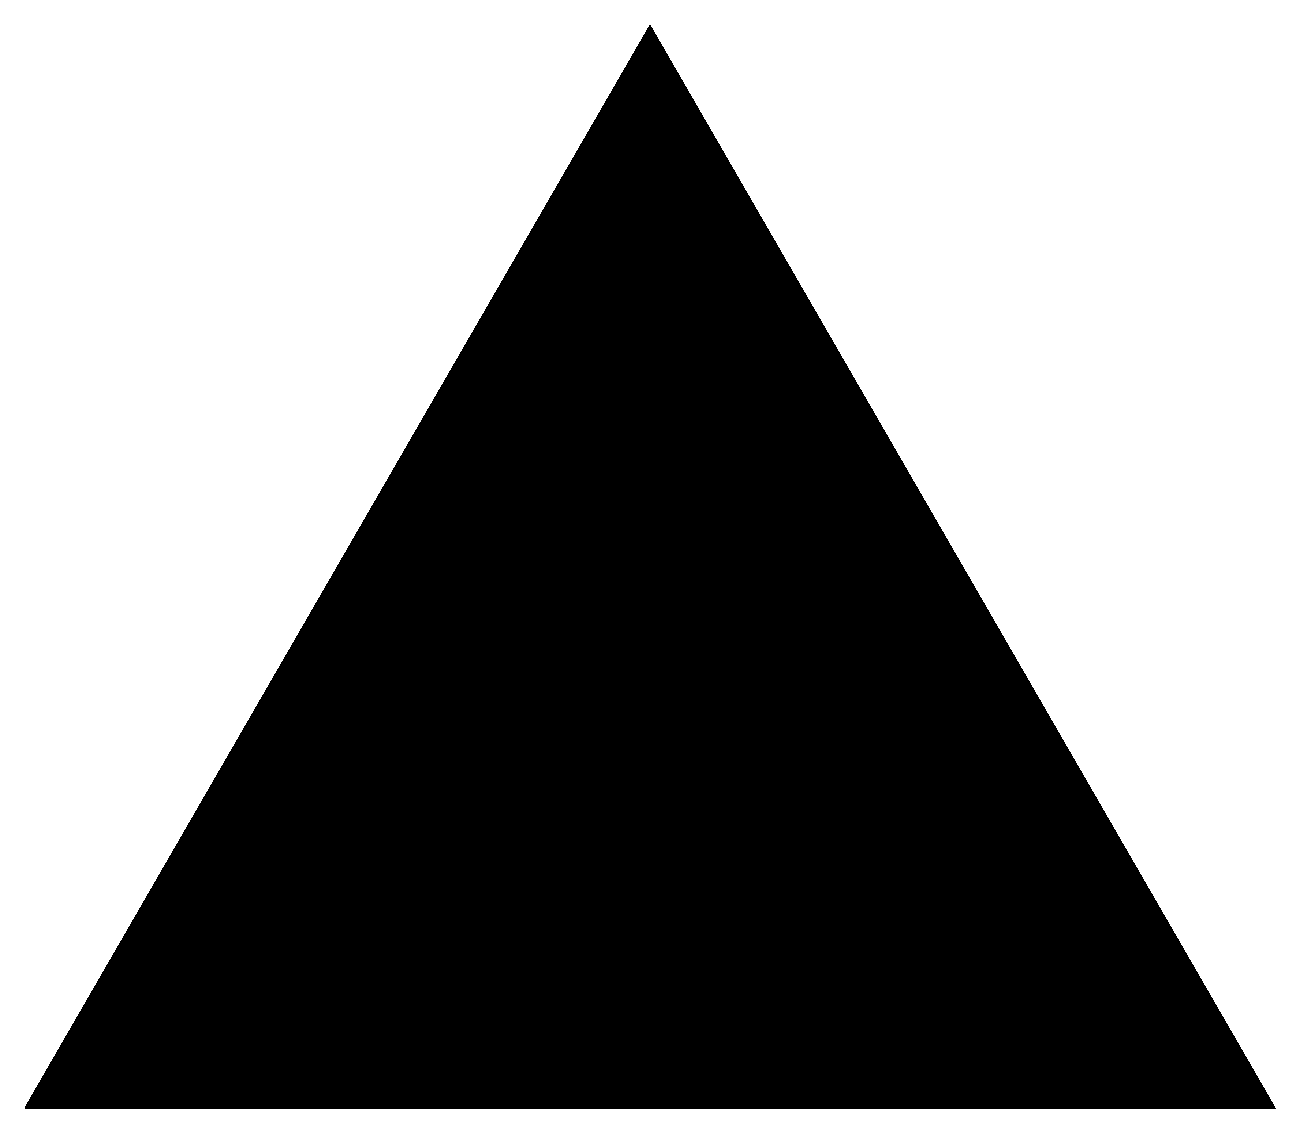
\includegraphics[width=0.4\textwidth]{ch01-sierpinskeho-trojuhelnik-0iterace.pdf}\qquad
    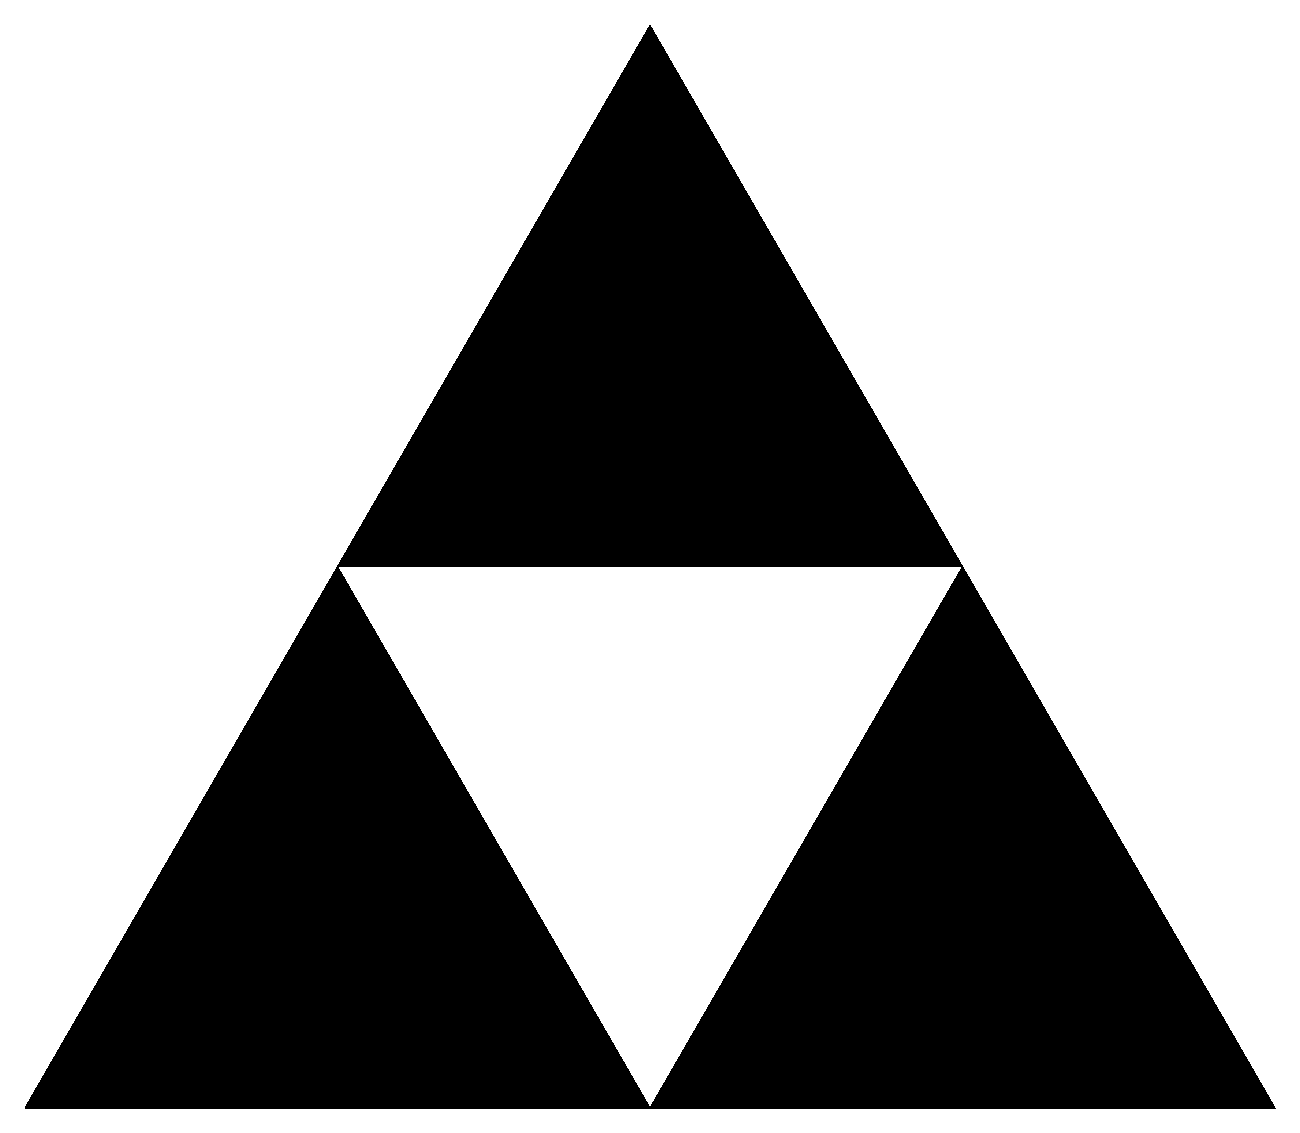
\includegraphics[width=0.4\textwidth]{ch01-sierpinskeho-trojuhelnik-1iterace.pdf}\qquad\\
    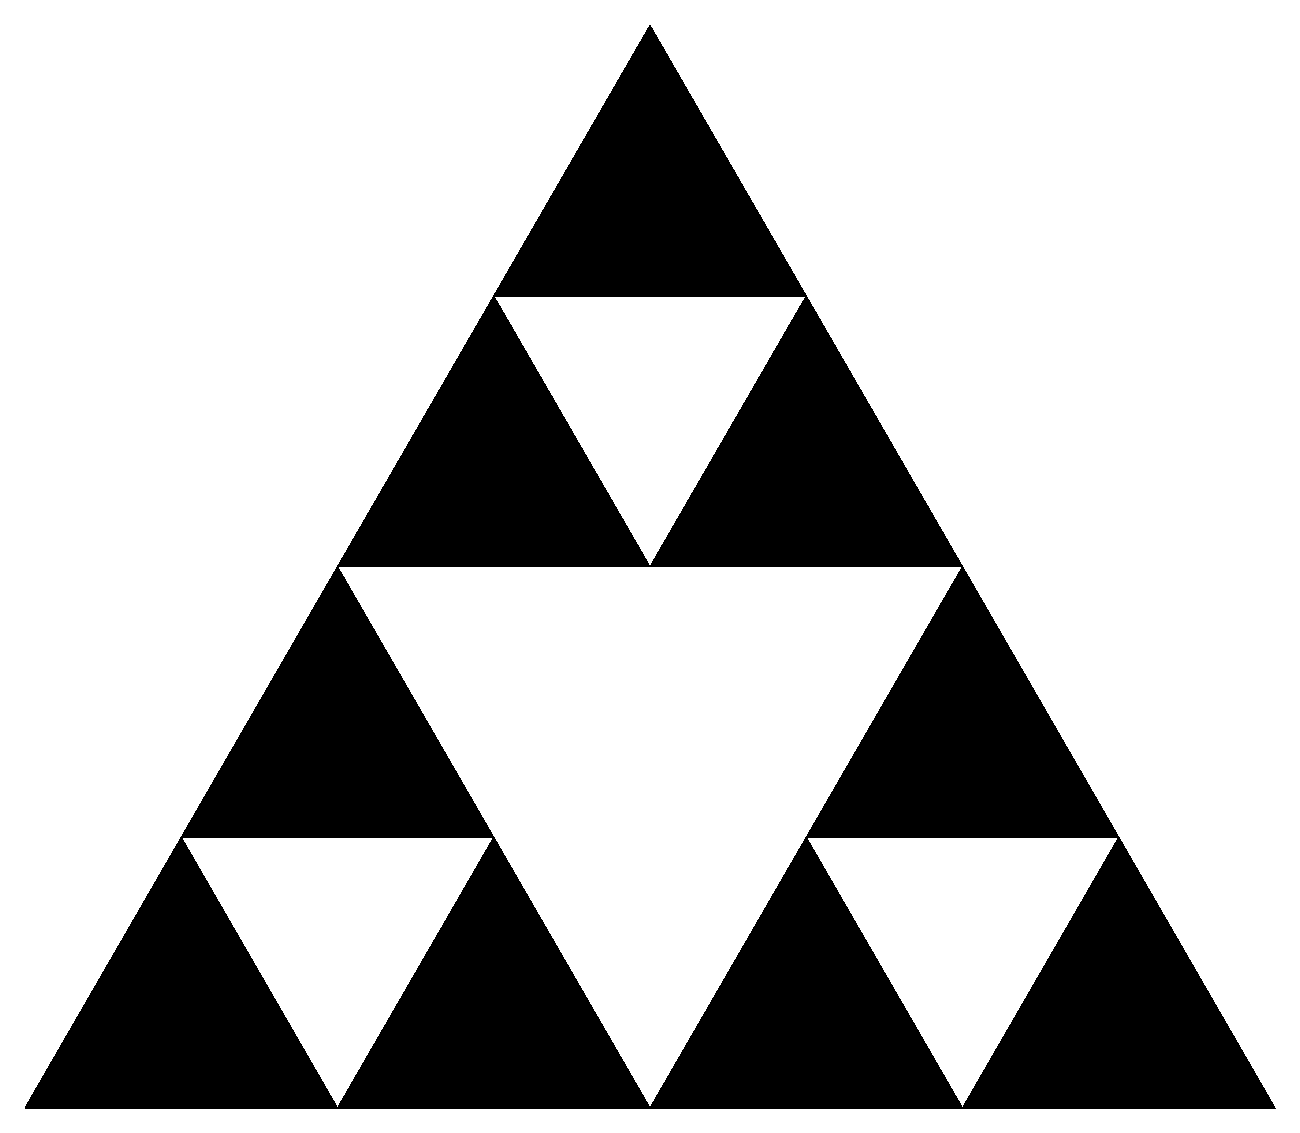
\includegraphics[width=0.4\textwidth]{ch01-sierpinskeho-trojuhelnik-2iterace.pdf}\qquad
    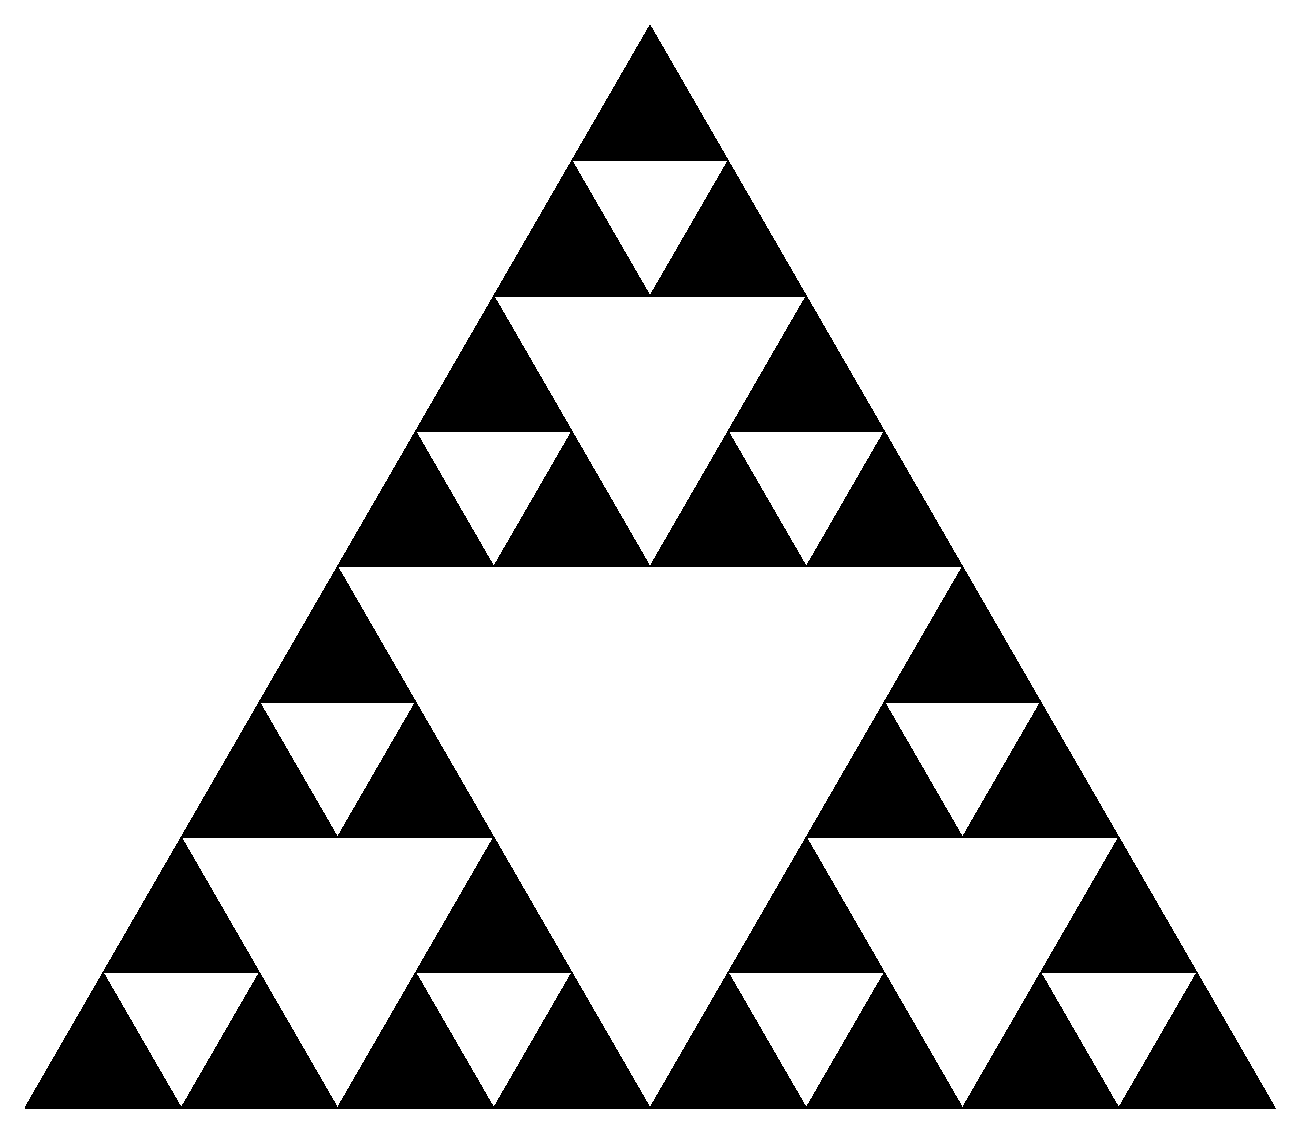
\includegraphics[width=0.4\textwidth]{ch01-sierpinskeho-trojuhelnik-3iterace.pdf}\qquad\\
    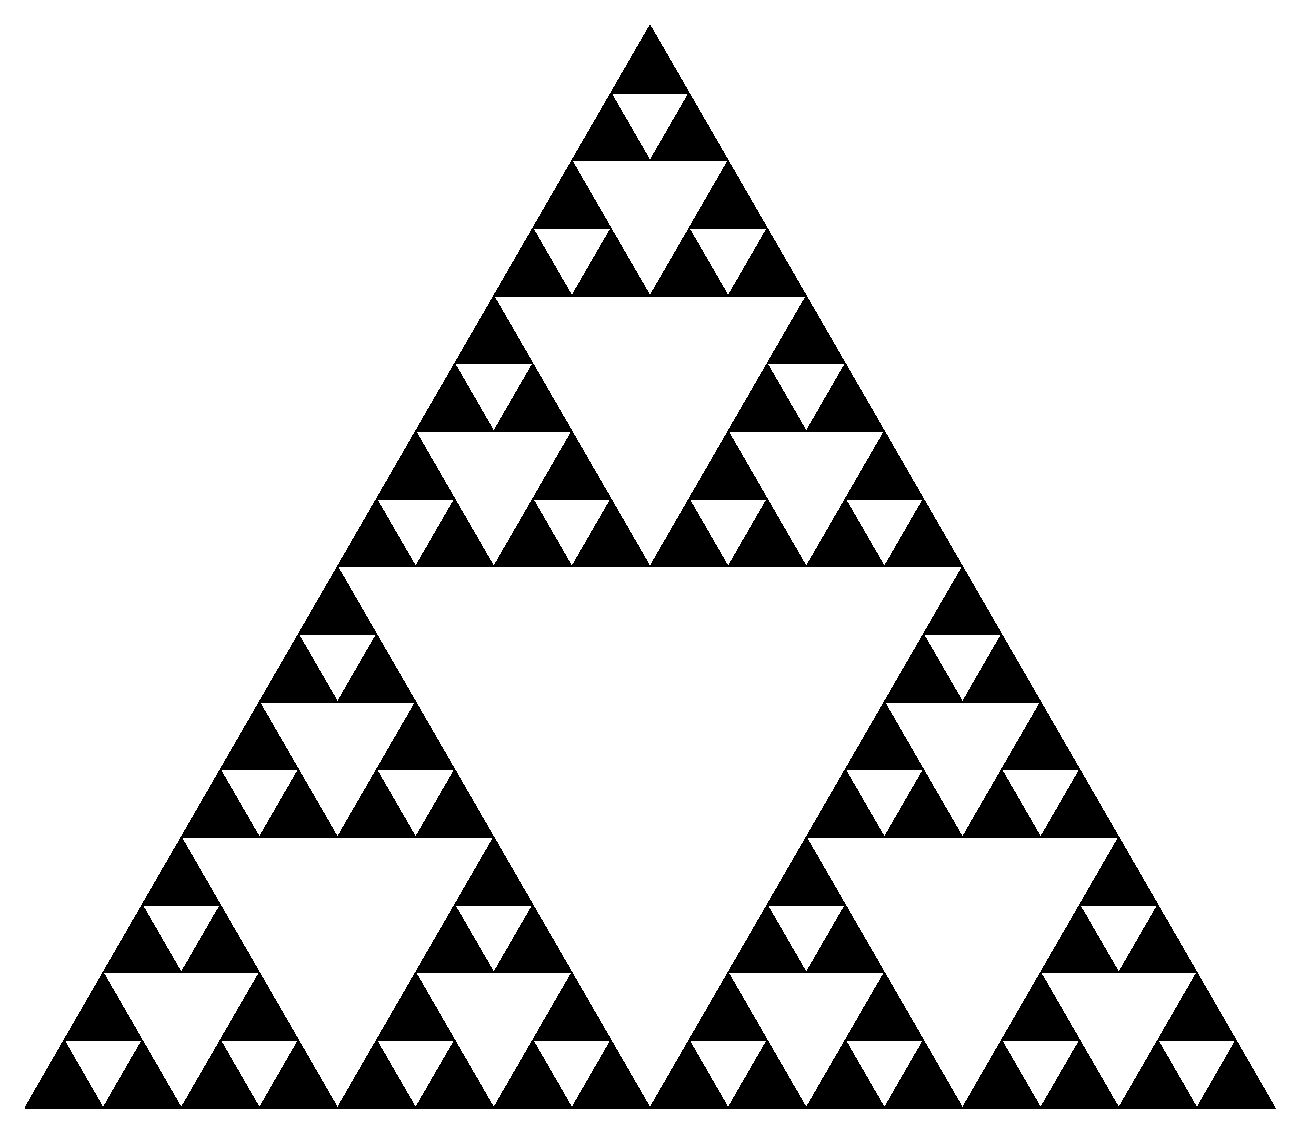
\includegraphics[width=0.4\textwidth]{ch01-sierpinskeho-trojuhelnik-4iterace.pdf}
    \caption{První čtyři iterace Sierpińského trojúhelníka.}
    \label{fig:sierpinskeho-trojuhelnik-5iteraci}
\end{figure}
I zde si lze všimnout,~že po nekonečně mnoha iteracích budou menší trojúhelníky přesnými kopiemi původního obrazce. Zkusme se opět podívat,~jak je to s~obvodem obrazce. Každá ze středních příček,~které vzniknou v~další iteraci,~má poloviční délku vůči délce strany $l$ původního trojúhelníku. Obvod obrazce se tak zvětší o~$3l/2$. Počet trojúhelníků poroste exponenciálně,~neboť v~každé iteraci odstraněním jednoho trojúhelníku vzniknou tři nové,~tj. obvod se po $k$-té iteraci zvětší o~$3^k\cdot(1/2)^k=(3/2)^k$ (na začátku pro $k=0$ je obvod $3$). Obvod obrazce $O_n$ po $n$ iteracích bude roven součtu přírůstků přes všechny iterace,~tj.
\begin{equation}\label{eq:obvod_sierpinskeho_trojuhelniku_niteraci}
    O_n=3+\sum_{k=1}^n{\left(\dfrac{3}{2}\right)^k}.
\end{equation}
Řada $\sum_{k=1}^{n}(3/2)^k$ je geometrická s~kvocientem $3/2$. Zde si vzpomeňme na vzorec pro její součet.
\begin{theorem}[Součet geomerické řady]\label{thm:soucet_geometricke_rady}
    Nechť je dána geometrická posloupnost $\{g_k\}_{k=1}^\infty$ s~kvocientem $q\neq 1$. Pak pro součet prvních $n$ členů platí
    \begin{equation*}
        \sum_{k=1}^{n}{g_k}=g_1\dfrac{1-q^n}{1-q}.
    \end{equation*}
\end{theorem}
\begin{proof}
    Důkaz vzorce zde vynecháme,~nicméně čtenář si jej může snadno ověřit např. indukcí podle $n$. 
\end{proof}
Celkově tak po aplikaci vzorce z~\ref{thm:soucet_geometricke_rady} v~rovnosti \eqref{eq:obvod_sierpinskeho_trojuhelniku_niteraci} dostaneme po jednoduché úpravě
\begin{equation*}
    O_n=3+\sum_{k=1}^n{\left(\dfrac{3}{2}\right)^k}=3+\dfrac{3}{2}\cdot\dfrac{\left(\dfrac{3}{2}\right)^n-1}{\dfrac{3}{2}-1}=3+3\left(\left(\dfrac{3}{2}\right)^n-1\right)=3\left(\dfrac{3}{2}\right)^n.
\end{equation*}
Posloupnost $\{O_n\}_{n=0}^\infty$ je opět geometrická s~kvocientem $q=3/2>1$,~tzn. její limita je opět $\infty$. Obvod Sierpińského trojúhelníku\index{Sierpińského trojúhelník}\index{trojúhelník!Sierpińského} tedy roste nade všechny meze. (Výpočet jsme si mohli též zjednodušit uvědoměním si,~že obvod obrazce roste s~faktorem $3/2$ a vzorec pro $O_n$ jsme tak mohli určit ihned.)\par
Podívejme se nyní na obsah útvaru. Zde si již výpočet trochu usnadníme. Po každé iteraci se jeho obsah zmenší na $3/4$ obsahu původního obrazce. Lze snadno odvodit,~že obsah rovnostranného trojúhelníku o~straně délky $a$ je
\begin{equation*}
    \dfrac{\sqrt{3}}{4}a^2
\end{equation*}
Na začátku je obsah útvaru $S_0=\sqrt{3}/4$. Tj. celkově po $n$-iteracích bude obsah $S_n$ roven
\begin{equation}\label{eq:obsah_sierpinskeho_trojuhelniku}
    \dfrac{\sqrt{3}}{4}\left(\dfrac{3}{4}\right)^n
\end{equation}
Výraz \eqref{eq:obsah_sierpinskeho_trojuhelniku} má pro $n\to\infty$ limitu nulovou,~tedy zatímco Sierpińského trojúhelník má \emph{nekonečný obvod},~jeho obsah je však naopak \emph{nulový}.

\subsection{Kochova vločka}\label{subsec:kochova_vlocka}
Rozšiřující variantou Kochovy křivky \ref{subsec:kochova_krivka} je tzv. \emph{Kochova vločka}\index{Kochova vločka}\index{vločka!Kochova},~která se skládá ze tří Kochových křivek\index{Kochova křivka}\index{křivka!Kochova}. Rozdíl je zde v~tom,~že začínáme s~rovnostranným trojúhelníkem o~straně délky $1$. Na každou ze stran aplikujeme stejný proces,~jako předtím,~tj. odebereme prostřední třetinu,~nahradíme ji dvěma na sebe navazujícími úsečkami délek $1/3$ a opakujeme pro každou nově vzniklou úsečku (viz obrázky \ref{fig:kochova_vlocka_dve_iterace} a \ref{fig:kochova_krivka_5iterace}).
\begin{figure}[h]
    \centering
    \begin{subfigure}{\subfigwidth}
        \centering
        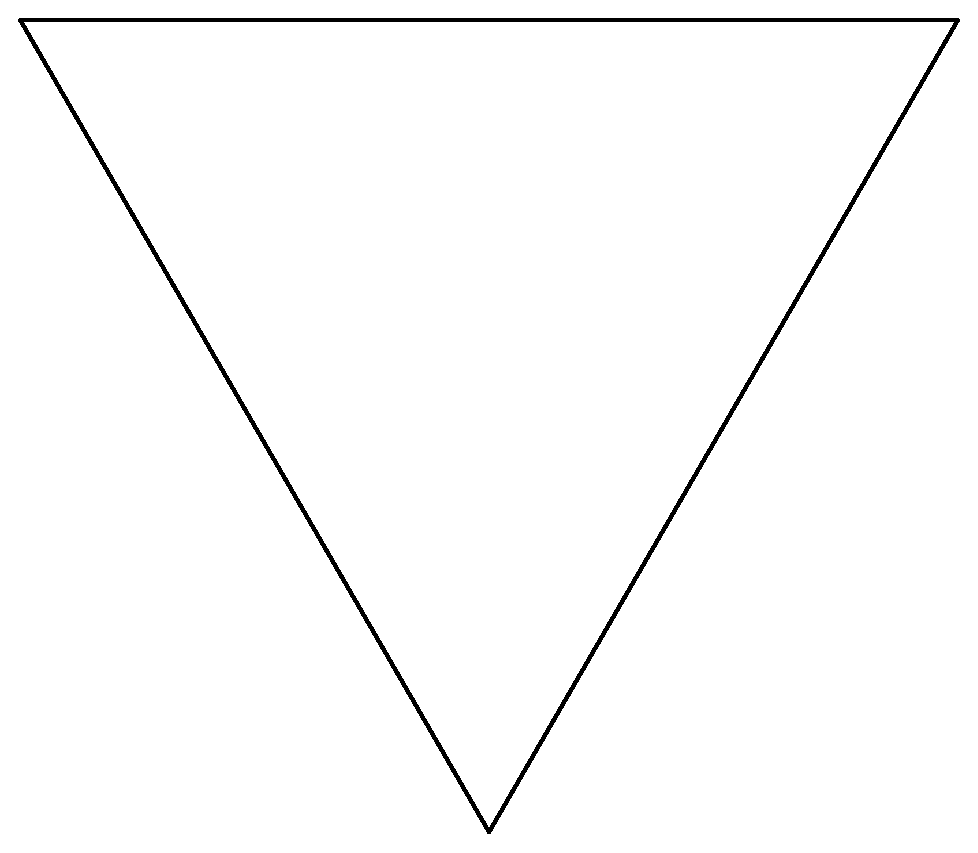
\includegraphics[scale=\fractalscale]{ch01-kochova-vlocka-0iterace.pdf}
    \end{subfigure}
    \qquad
    \begin{subfigure}{\subfigwidth}
        \centering
        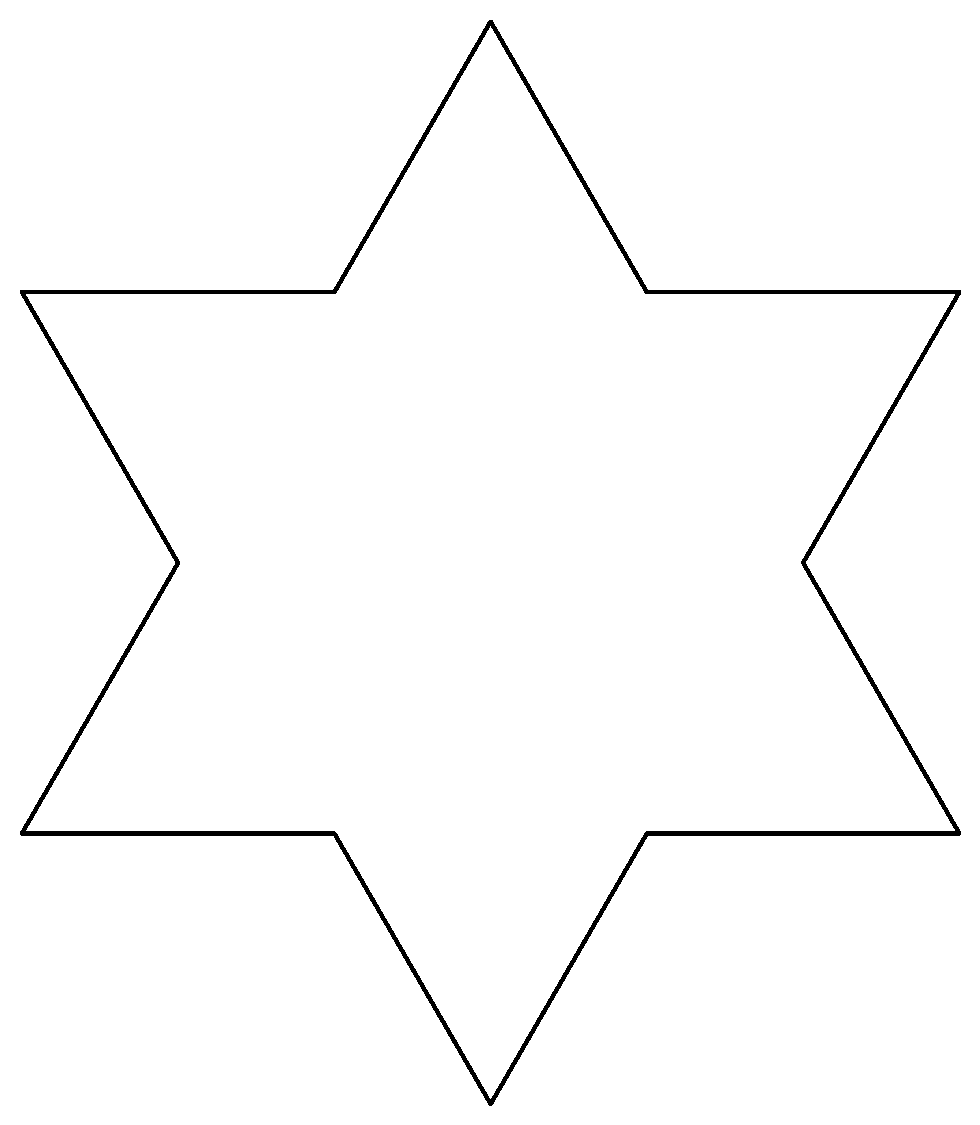
\includegraphics[scale=\fractalscale]{ch01-kochova-vlocka-1iterace.pdf}
    \end{subfigure}
    \caption{Nultá a první iterace Kochovy vločky.}
    \label{fig:kochova_vlocka_dve_iterace}
\end{figure}
\begin{figure}[h]
    \centering
    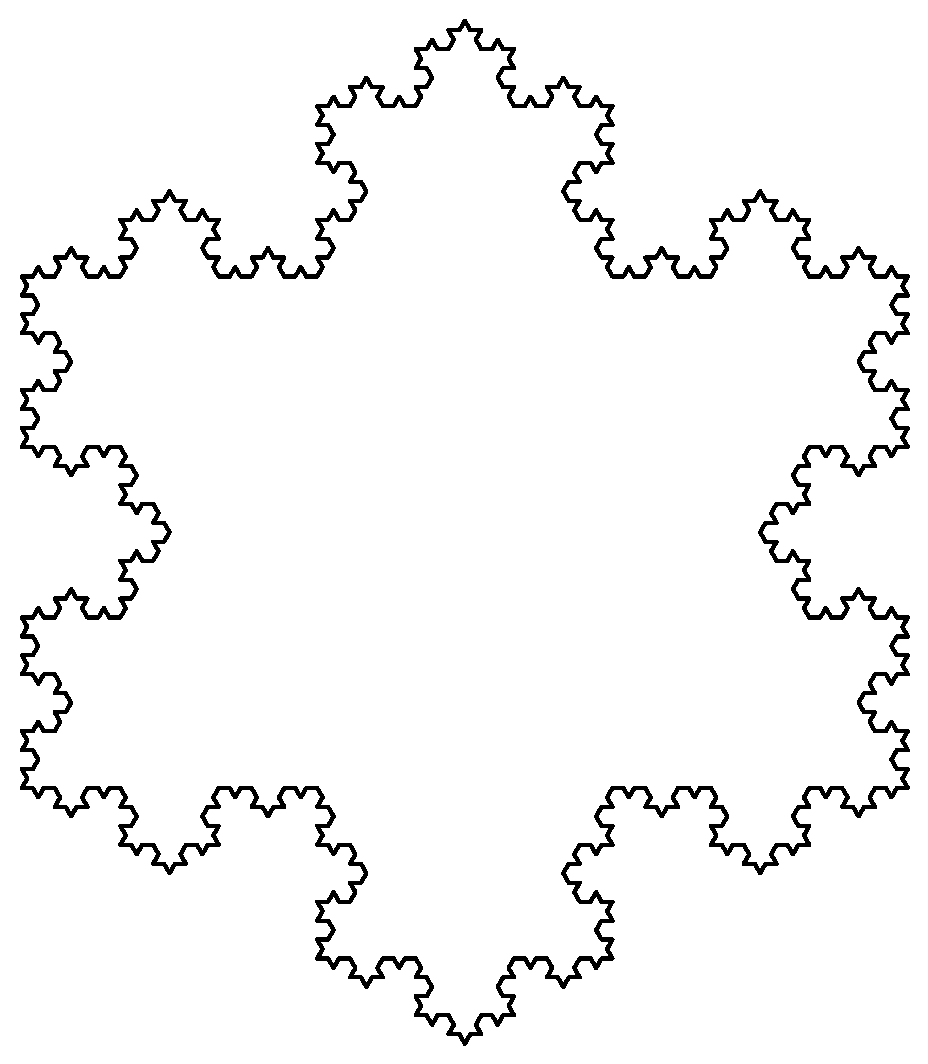
\includegraphics[scale=\fractalscale]{ch01-kochova-vlocka-4iterace.pdf}
    \caption{Čtvrtá iterace Kochovy vločky.}
    \label{fig:kochova_krivka_5iterace}
\end{figure}
Podíváme-li se na obvod,~nejspíše nás nepřekvapí,~že ten je i~zde nekonečný\footnote{Obvod Kochovy křivky po $n$-té iteraci je $o_n=3\cdot(4/3)^{n}$.} (už z~principu,~že každá strana původního rovnostranného trojúhelníka představuje samostatnou Kochovu křivku).
Obsah vzniklého útvaru je však již zajímavější. Pro zjednodušení výpočtu si rozdělme útvar na \emph{stejné rovnostranné trojúhelníky} podle obrázku \ref{fig:kochova_vlocka_rozdeleni},~jejichž obsah je roven $1/12$ obsahu obrazce v~nulté iteraci.
\begin{figure}[h]
    \centering
    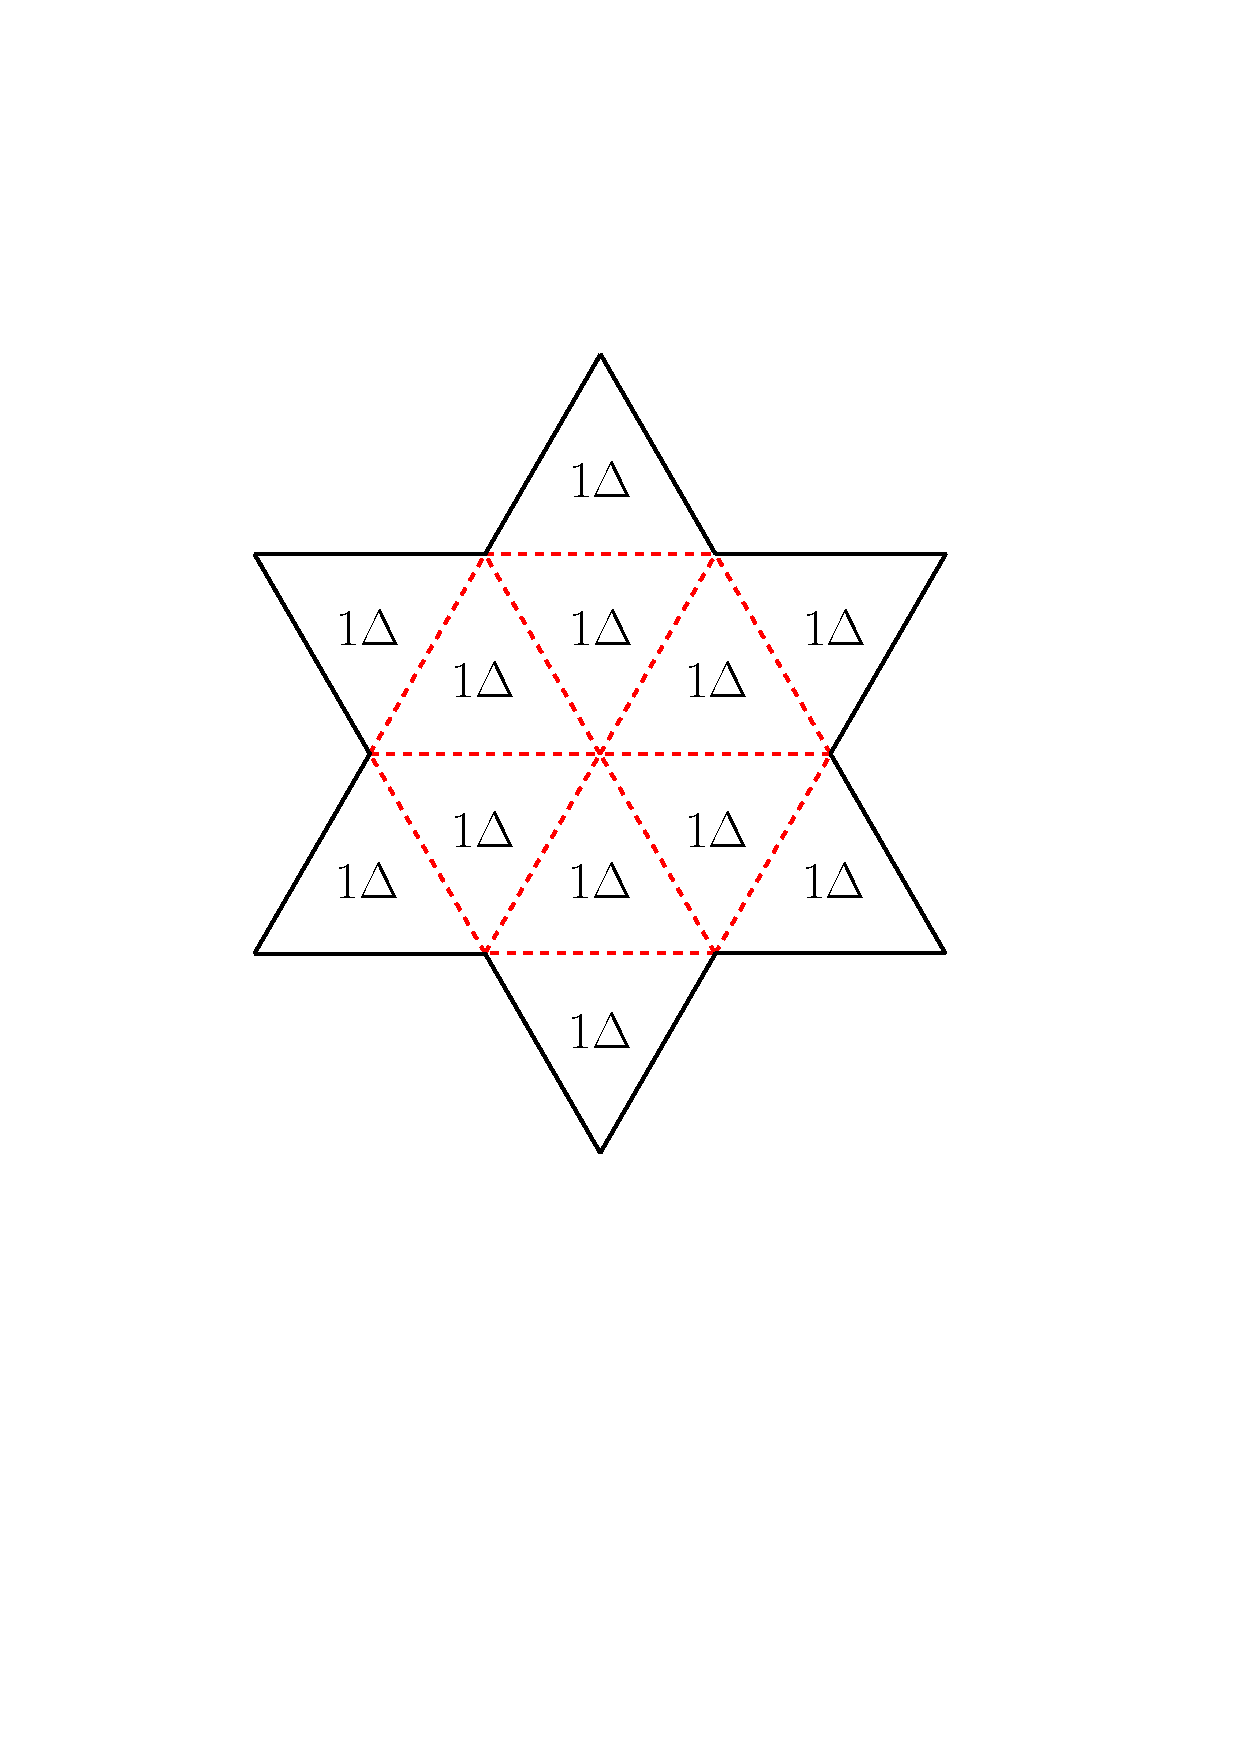
\includegraphics[scale=.4]{ch01-kochova-vlocka-rozdeleni.pdf}
    \caption{Rozdělení první iterace Kochovy vločky.}
    \label{fig:kochova_vlocka_rozdeleni}
\end{figure}
Výsledný obsah se tedy pokusíme vyjádřit relativně vůči \emph{obsahům daných trojúhelníků},~na něž jsme obrazec rozdělili,~a pak jej pouze přepočítáme. Jejich obsah si označme $\Delta$. Tedy obsah Sierpińského trojúhelníku v~nulté iteraci lze vyjádřit jako $S_0=9\Delta$. Po první iteraci vzniknou na každé ze strany 3 nové trojúhelníky o~obsahu $1/9\cdot\Delta$. V~každé další iteraci vzniknou z~jedné úsečky 4 nové. Obecně po $n$ iteracích jich tedy bude $3\cdot 4^{n}$. (Při výpočtu musíme počítat s~o jedna nižší mocninou,~neboť trojúhelníky vznikají "na úsečkách" z~předešlé iterace,~nikoliv té aktuální.)\par
Zaměřme se nyní pouze trojúhelníky,~které vznikly v~aktuální iteraci (viz obrázek \ref{fig:kochova_vlocka_2iterace_nove_trojuhelniky}). Součet jejich obsahů nám dává \emph{přírůstek obsahu} v~obecné $n$-té iteraci. Označíme-li tento přírůstek $B_n$,~pak platí
\[B_n=\underbrace{3\cdot 4^{n-1}}_{\text{počet úseček}}\cdot\overbrace{\left(\dfrac{1}{9}\right)^{n-1}\Delta}^{\text{obsah nových troj.}}=3\cdot\left(\dfrac{4}{9}\right)^{n-1}\Delta,\]
kde $n\geqslant 1$.
\begin{figure}[h]
    \centering
    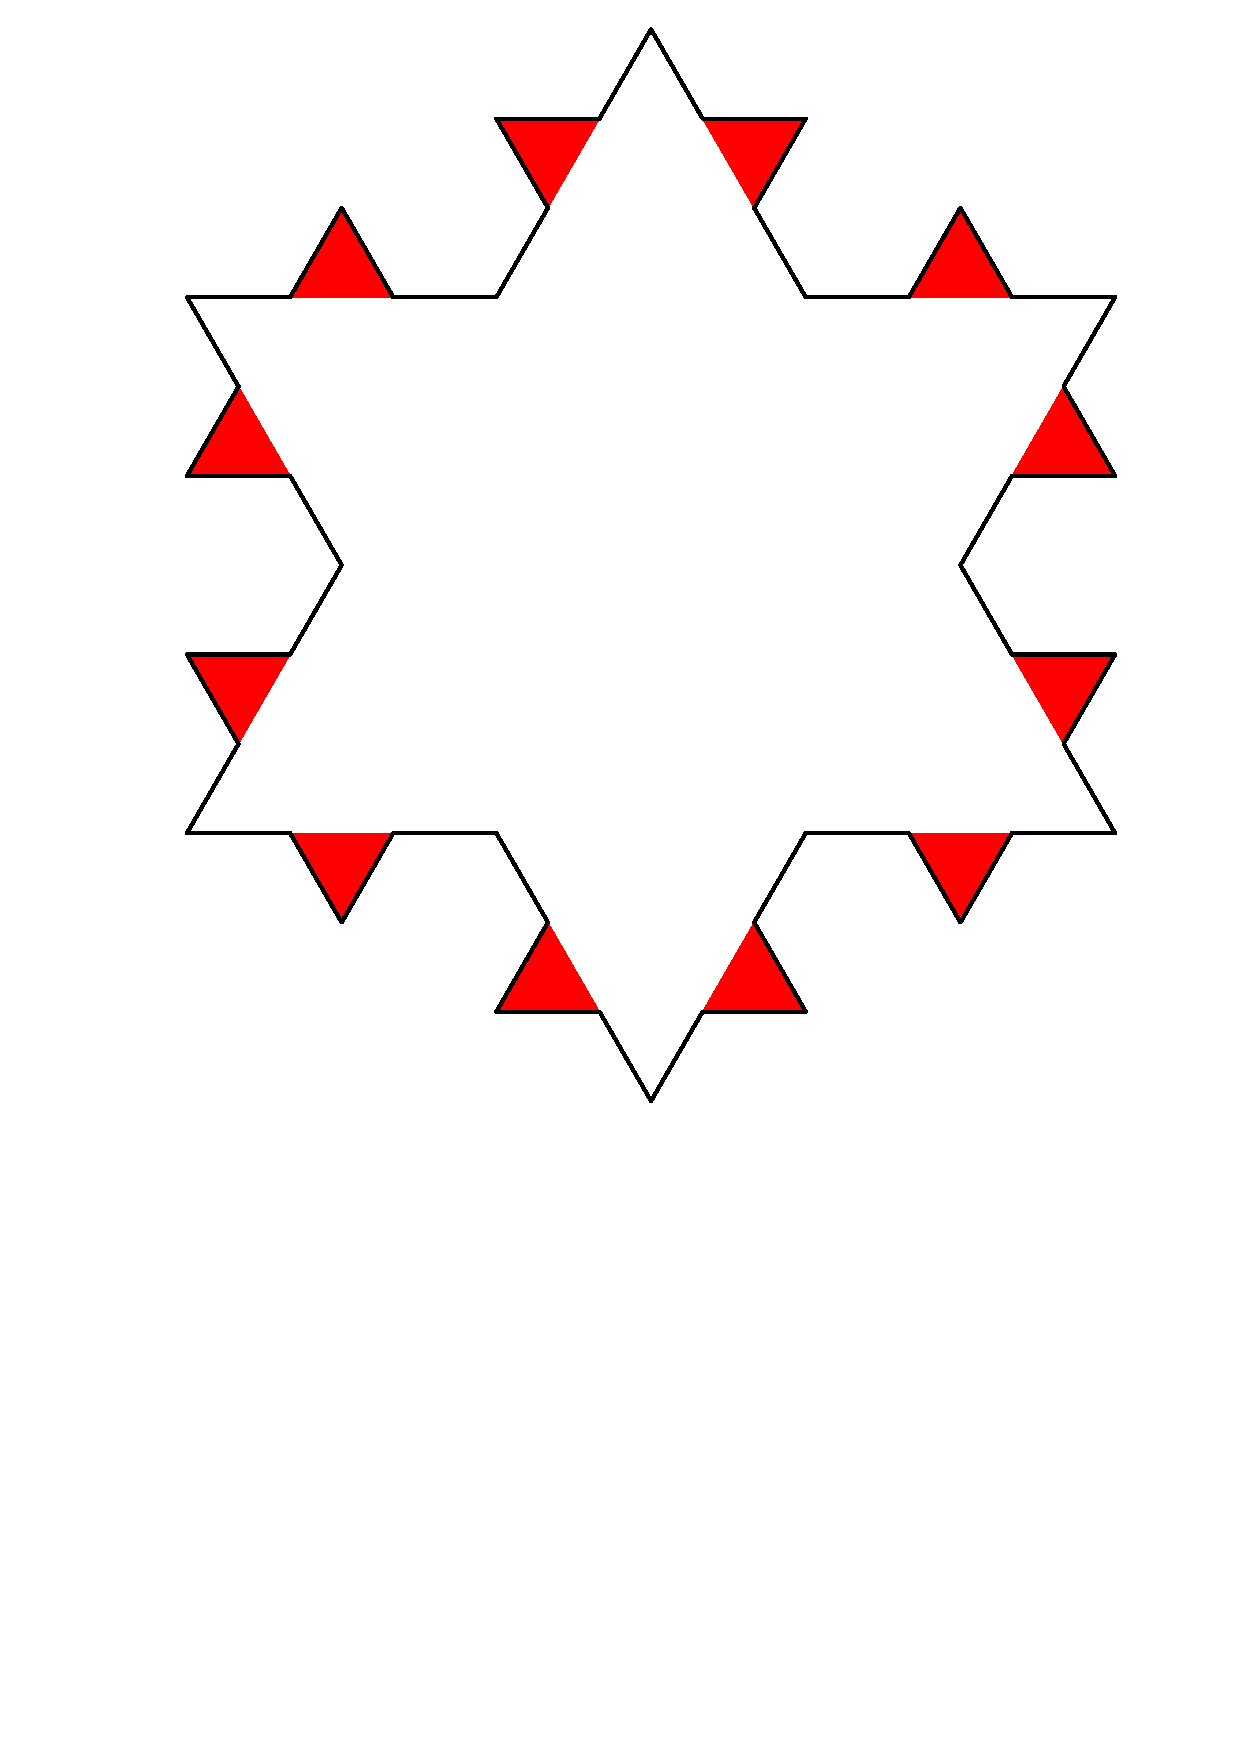
\includegraphics[scale=\fractalscale]{ch01-kochova-vlocka-2iterace-nove-trojuhelniky.pdf}
    \caption{Nově vzniklé trojúhelníky v~druhé iteraci.}
    \label{fig:kochova_vlocka_2iterace_nove_trojuhelniky}
\end{figure}
Nyní můžeme již vyšetřit obsah v~$n$-té iteraci $S_n$ a posléze i~celkový obsah výsledného obrazce $S=\lim_{n\to\infty}{S_n}$. Pro $n\geqslant 1$ platí
\begin{align*}
    S_n&=S_0+\sum_{k=1}^{n}{B_k}=9\Delta+3\Delta\cdot\sum_{k=1}^{n}{\left(\dfrac{4}{9}\right)^{k-1}}=9\Delta+3\Delta\cdot\dfrac{1-\left(\dfrac{4}{9}\right)^{n}}{1-\dfrac{4}{9}}\\
    &=9\Delta+\dfrac{27}{5}\Delta\cdot\left(1-\left(\dfrac{4}{9}\right)^n\right)
\end{align*}
Tedy
\begin{align*}
    S&=\lim_{n\to\infty}{S_n}=9\Delta+\dfrac{27}{5}\Delta\cdot\left(1-\left(\dfrac{4}{9}\right)^n\right)=9\Delta+\dfrac{27}{5}\Delta\cdot\left(1-\lim_{n\to\infty}\left(\dfrac{4}{9}\right)^n\right)\\
    &=9\Delta+\dfrac{27}{5}\Delta=\dfrac{72}{5}\Delta.
\end{align*}
Obsah trojúhelníků,~na než jsme rozdělili první iteraci Kochovy vločky,~je
\[\Delta=\dfrac{\sqrt{3}}{4}\cdot\dfrac{1}{9}\]
a tedy celkově
\[S=\dfrac{72}{5}\Delta=\dfrac{72}{5}\cdot\dfrac{\sqrt{3}}{4}\cdot\dfrac{1}{9}=\dfrac{2\sqrt{3}}{5}.\]
Byl to trochu delší výpočet,~nicméně jsme zjistili,~že Kochova vločka má (stejně jako Kochova křivka) \emph{nekonečnou délku (obvod)},~ale obsah má \emph{konečný}.
% Obsah vzniklého útvaru je však již zajímavější. Po první iteraci přibudou 3 nové trojúhelníky se stranou délky $1/3$,~tzn. jejich obsah bude
% \begin{equation*}
%     \dfrac{\sqrt{3}}{4}\left(\dfrac{1}{3}\right)^2
% \end{equation*}
% a celkový obsah obrazce tedy bude
% \begin{equation*}
%     S_1=\dfrac{\sqrt{3}}{4}+3\cdot\dfrac{\sqrt{3}}{4}\left(\dfrac{1}{3}\right)^2.
% \end{equation*}
% V~každé další iteraci vzniknou z~jedné úsečky 4 nové. Obecně po $n$ iteracích jich bude $3\cdot 4^n$ (při výpočtu však musíme počítat s~o jedna nižší mocninou,~neboť trojúhelníky vznikají "na úsečkách" z~předešlé iterace,~nikoliv té aktuální,~viz obrázek \ref{fig:kochova_vlocka_2iterace_nove_trojuhelniky}).
% \begin{figure}[h]
%     \centering
%     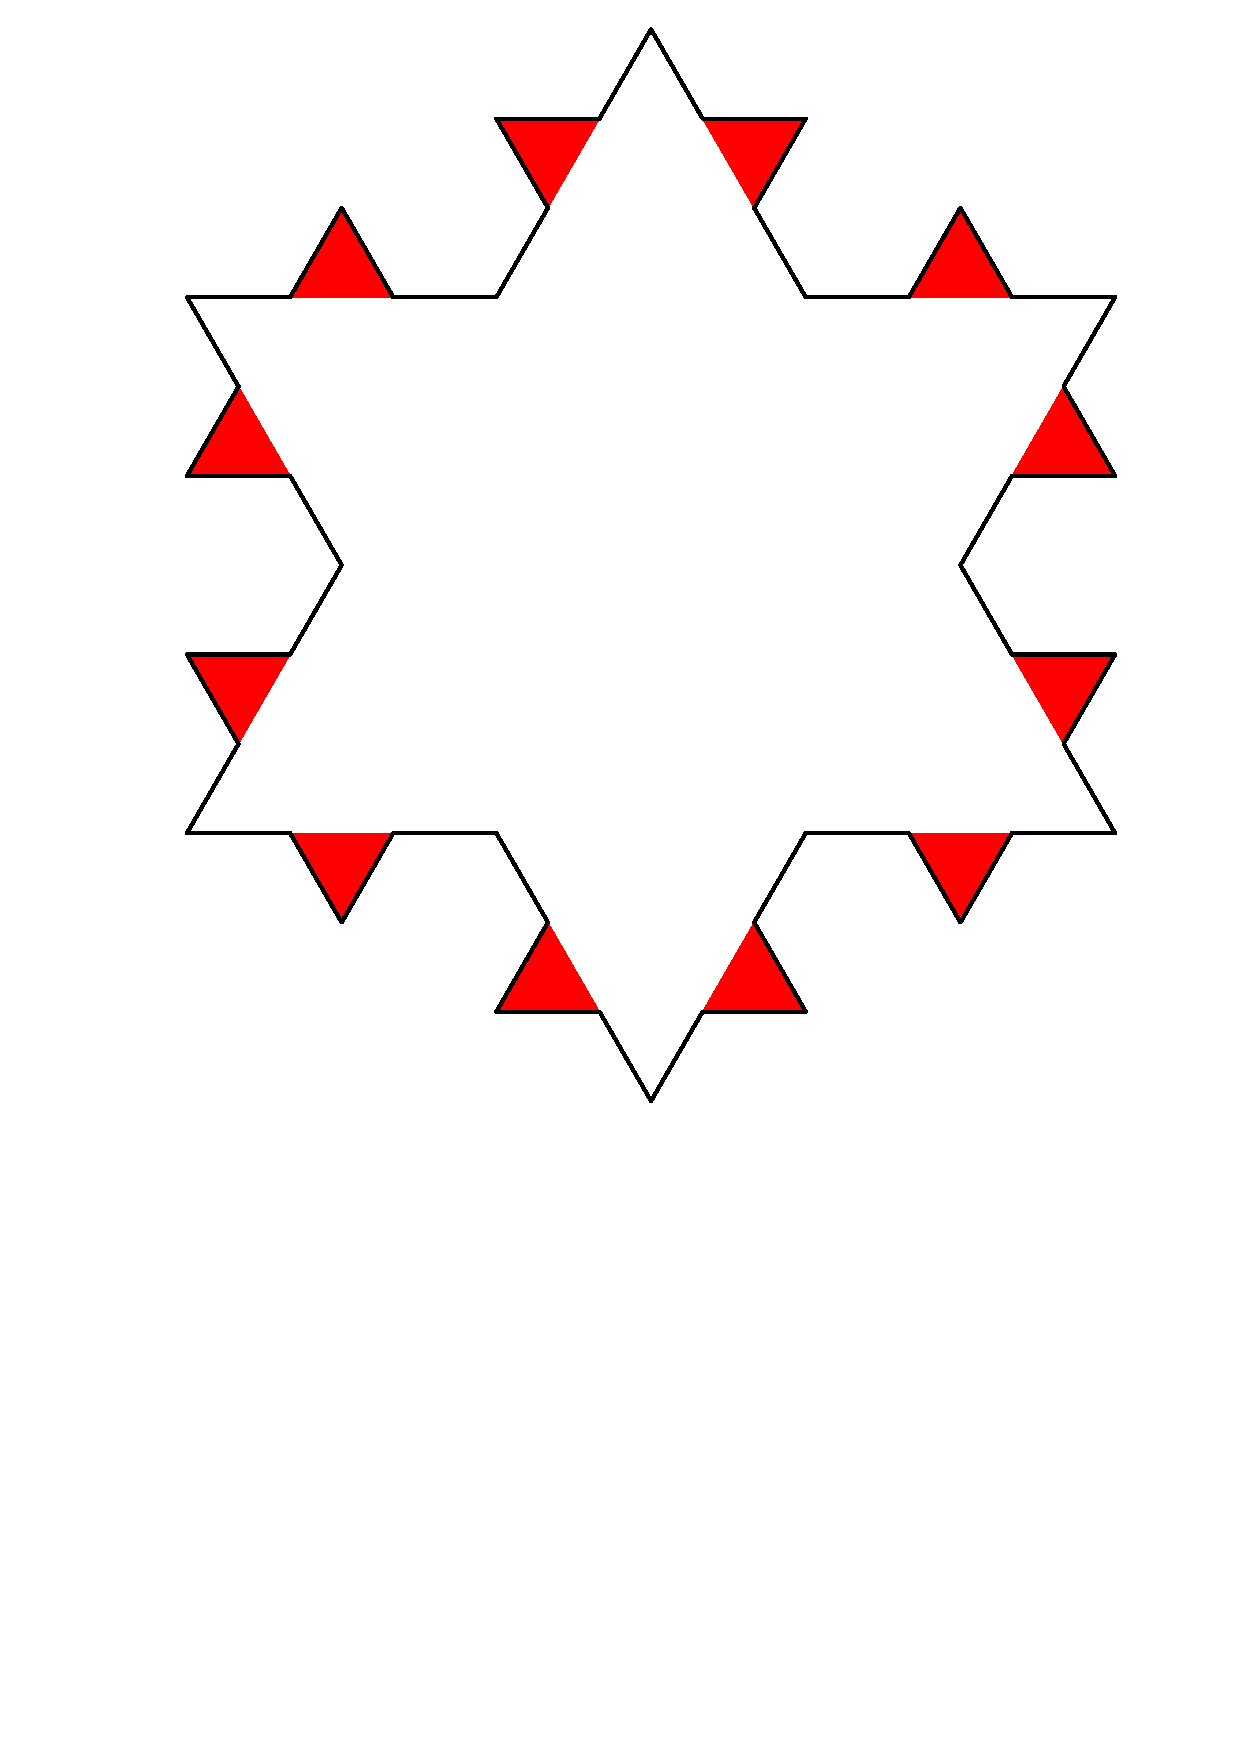
\includegraphics[scale=\fractalscale]{ch01-kochova-vlocka-2iterace-nove-trojuhelniky.pdf}
%     \caption{Nově vzniklé trojúhelníky v~druhé iteraci.}
%     \label{fig:kochova_vlocka_2iterace_nove_trojuhelniky}
% \end{figure}
% Délka úseček,~a tedy i~stran nově vzniklých rovnostranných trojúhelníků,~je $(1/3)^n$. Celkový obsah nově vzniklých trojúhelníků je tak
% \begin{equation}\label{eq:obsah_novych_trojuhelniku}
%     3\cdot 4^{n-1}\cdot\dfrac{\sqrt{3}}{4}\left(\dfrac{1}{3^n}\right)^2.
% \end{equation}
% Pro další výpočet bude pro nás výhodné si výraz \eqref{eq:obsah_novych_trojuhelniku} upravit.
% \begin{equation*}
%     3\cdot 4^{n-1}\cdot\dfrac{\sqrt{3}}{4}\left(\dfrac{1}{3^n}\right)^2=\dfrac{3\sqrt{3}}{4^2}\cdot \dfrac{4^n}{3^{2n}}=\dfrac{3\sqrt{3}}{16}\left(\dfrac{4}{9}\right)^n.
% \end{equation*}
% Celkový obsah obrazce po $n$ iteracích lze tak vypočítat součtem obsahů všech vzniklých trojúhelníků ve všech předešlých iteracích,~tj.
% \begin{equation*}
%     S_n=\sum_{k=1}^n{S_k}=\overbrace{\dfrac{\sqrt{3}}{4}}^{S_0}+\sum_{k=1}^n{\dfrac{3\sqrt{3}}{16}\left(\dfrac{4}{9}\right)^k}.
% \end{equation*}
% Suma na pravé straně představuje geometrickou řadu s~kvocientem $4/9$. Úpravou získáme
% \begin{equation}\label{eq:kochova_vlocka_obsah_n_iteraci}
%     \dfrac{\sqrt{3}}{4}+\dfrac{3\sqrt{3}}{16}\sum_{k=1}^n{\left(\dfrac{4}{9}\right)^k}=\dfrac{\sqrt{3}}{4}+\dfrac{3\sqrt{3}}{16}\cdot\dfrac{4}{9}\cdot\dfrac{1-\left(\dfrac{4}{9}\right)^n}{1-\dfrac{4}{9}}=\dfrac{\sqrt{3}}{4}+\dfrac{3\sqrt{3}}{20}\left(1-\left(\dfrac{4}{9}\right)^n\right)
% \end{equation}
% Můžeme si všimnout,~že výraz \eqref{eq:kochova_vlocka_obsah_n_iteraci} bude tentokrát již konečné číslo,~neboť limitním přechodem pro $n\to\infty$ se výraz $(4/9)^n$ bude blížit nule. Celkově tedy máme
% \begin{align*}
%     S&=\lim_{n\to\infty}S_n=\lim_{n\to\infty}\left(\dfrac{\sqrt{3}}{4}+\dfrac{3\sqrt{3}}{20}\left(1-\left(\dfrac{4}{9}\right)^n\right)\right)=\dfrac{\sqrt{3}}{4}+\dfrac{3\sqrt{3}}{20}\left(1-\lim_{n\to\infty}\left(\dfrac{4}{9}\right)^n\right)\\
%     &=\dfrac{\sqrt{3}}{4}+\dfrac{3\sqrt{3}}{20}=\dfrac{2\sqrt{3}}{5}.
% \end{align*}

\subsection{Cantorovo diskontinuum}\label{subsec:cantorovo_diskontinuum}
Podívejme se ještě na jeden typ fraktálního objektu,~kterým je tzv. \emph{Cantorovo diskontinuum}\footnote{Též se mu říká \emph{Cantorova množina} (angl. \emph{"Cantor set"})\index{Cantorovo diskontinuum}\index{diskontinuum!Cantorovo}. Dvourozměrnou variantou je pak tzv. \emph{Cantorův prach}\index{Cantorův prach}\index{prach!Cantorův} (angl. \emph{"Cantor dust"}). Slovo \emph{prach} je zde míněno v~přeneseném významu,~neboť (podobně jako v~této podsekci) lze ukázat,~že vzniklé útvary mají v~limitě nulový obsah.} Myšlenka je zde velmi jednoduchá: začínáme s~úsečkou délky $1$ (nultá iterace) a následně odebereme prostřední třetinu,~čímž vznikne první iterace. V~dalších iteracích postupujeme analogicky pro vzniklé úsečky (viz obrázek \ref{fig:cantorovo_diskontinuum}).
\begin{figure}[h]
    \centering
    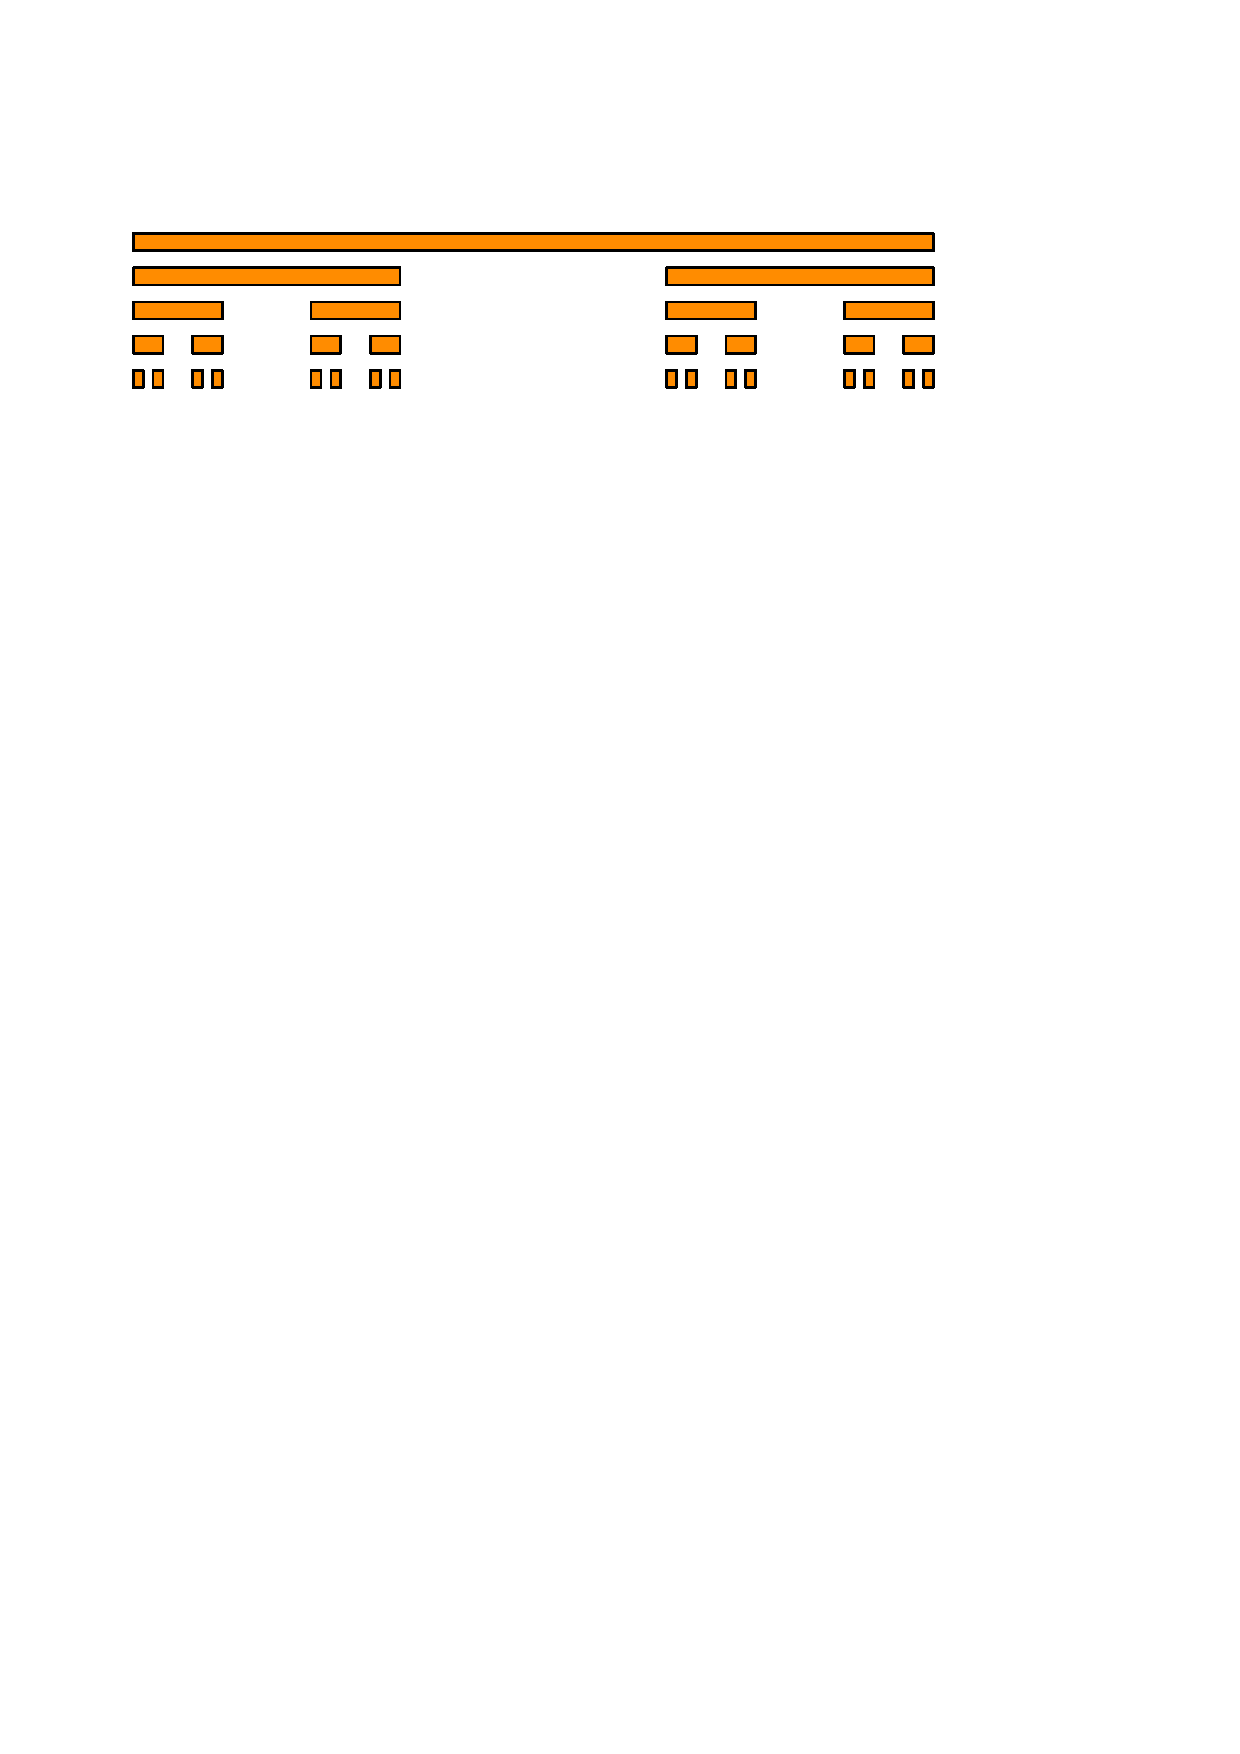
\includegraphics[scale=\normalipe]{ch01-cantorova-mnozina.pdf}
    \caption{Nultá až čtvrtá iterace Cantorova diskontinua.}
    \label{fig:cantorovo_diskontinuum}
\end{figure}

Nově vzniklé úsečky třetinové délky jsou kopiemi původní úsečky. Stejně jako u~předešlých fraktálů nás i~zde bude zajímat limitní chování tohoto procesu. Lze očekávat,~že postupným odebíráním zbudou úsečky nulové délky. O~tom se lze přesvědčit např. tak,~že spočítáme limitu celkových délek všech odebraných úseků. V~první iteraci odebereme úsečku délky $1/3$,~v~druhé iteraci odebereme dvě celkové délky $2\cdot(1/3)^2=2/9$,~ve třetí vyjmeme čtyři celkové délky $4\cdot(1/3)^3=4/27$,~atd. (viz obrázek \ref{fig:cantorovo_diskontinuum_delky}).
\begin{figure}[h]
    \centering
    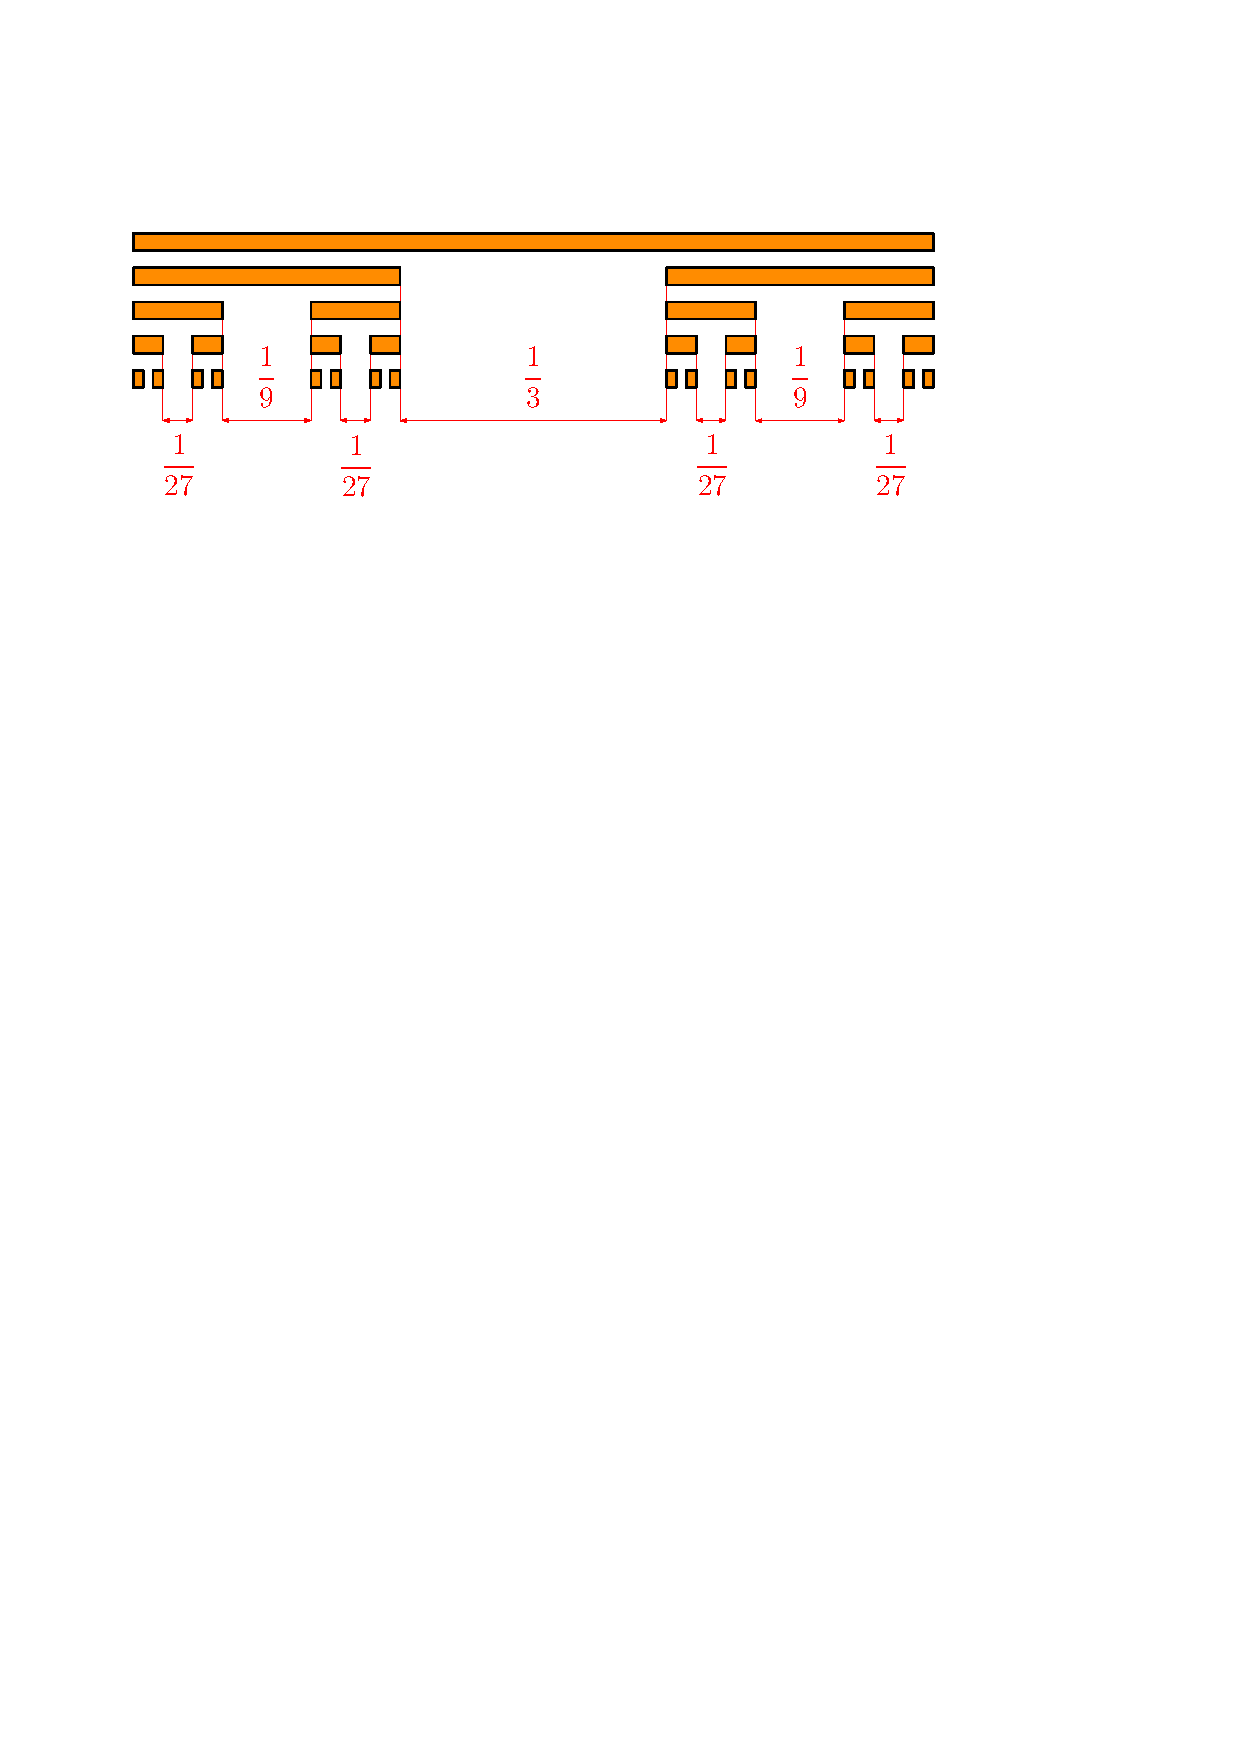
\includegraphics[scale=\normalipe]{ch01-cantorova-mnozina-delky.pdf}
    \caption{Znázornění délek vyjmutých úseků.}
    \label{fig:cantorovo_diskontinuum_delky}
\end{figure}
Obecně počet odebraných úseků roste s~mocninou dvojky,~jejichž délky klesají s~mocninou trojky,~tedy v~$n$-té iteraci odebereme úsek délky $2^n(1/3)^{n+1}$. Označíme-li tedy délku zbylých úseků $\ell_n$ po $n$ iteracích a $\overline{\ell_n}$ délku odebraných úseků,~pak určitě platí $\ell_n=1-\overline{\ell_n}$. Protože nás zajímá délka \emph{všech} odebraných úseků,~pak po $n$ iteracích bude celková délka rovna
\begin{equation}
    \overline{\ell_n}=\sum_{k=0}^{n}2^k\left(\dfrac{1}{3}\right)^{k+1}=\sum_{k=0}^{n}\dfrac{2^k}{3^{k+1}}=\dfrac{1}{3}\cdot\sum_{k=0}^{n}\left(\dfrac{2}{3}\right)^k=\dfrac{1}{3}\cdot\dfrac{1-\left(\dfrac{2}{3}\right)^{n+1}}{1-\dfrac{2}{3}}=1-\left(\dfrac{2}{3}\right)^{n+1}.
\end{equation}
Označíme-li si limitu výrazů posloupností $\ell_n$,~reps. $\overline{\ell_n}$,~jako $\ell$,~resp. $\overline{\ell}$,~pak dostaneme
\begin{equation*}
    \overline{\ell}=\lim_{n\to\infty}\overline{\ell_n}=\lim_{n\to\infty}\left(1-\left(\dfrac{2}{3}\right)^{n+1}\right)=1-\lim_{n\to\infty}\left(\dfrac{2}{3}\right)^{n+1}=1-0=1.
\end{equation*}
Z toho již triviálně plyne,~že
\begin{equation}
    \ell=\lim_{n\to\infty}\ell_n=\lim_{n\to\infty}(1-\overline{\ell_n})=1-\lim_{n\to\infty}\overline{\ell_n}=1-1=0,
\end{equation}
tzn. na konci procesu zbude Cantorovo diskontinuum délky nula.
\section{Fraktální dimenze}\label{sec:fraktalni_dimenze}

\subsection{Chápání konceptu dimenze}\label{subsec:koncept-dimenze}

Útvary vyčtené v~sekci~\ref{sec:sobepodobnost} ilustrují vlastnost soběpodobnosti,~kterou jsme si (zatím neformálně) popsali. V~eukleidovské geometrii lze však u~mnohých základních objektů pozorovat stejnou vlastnost. Např. čtverec lze určitě prohlásit v~jistém smyslu za soběpodobný,~neboť jej lze rozdělit na podobné útvary (viz obrázek~\ref{fig:sobepodobnost-ctverce}).
\begin{figure}[h]
    \centering
    \begin{subfigure}[b]{\subfigwidth}
        \centering
        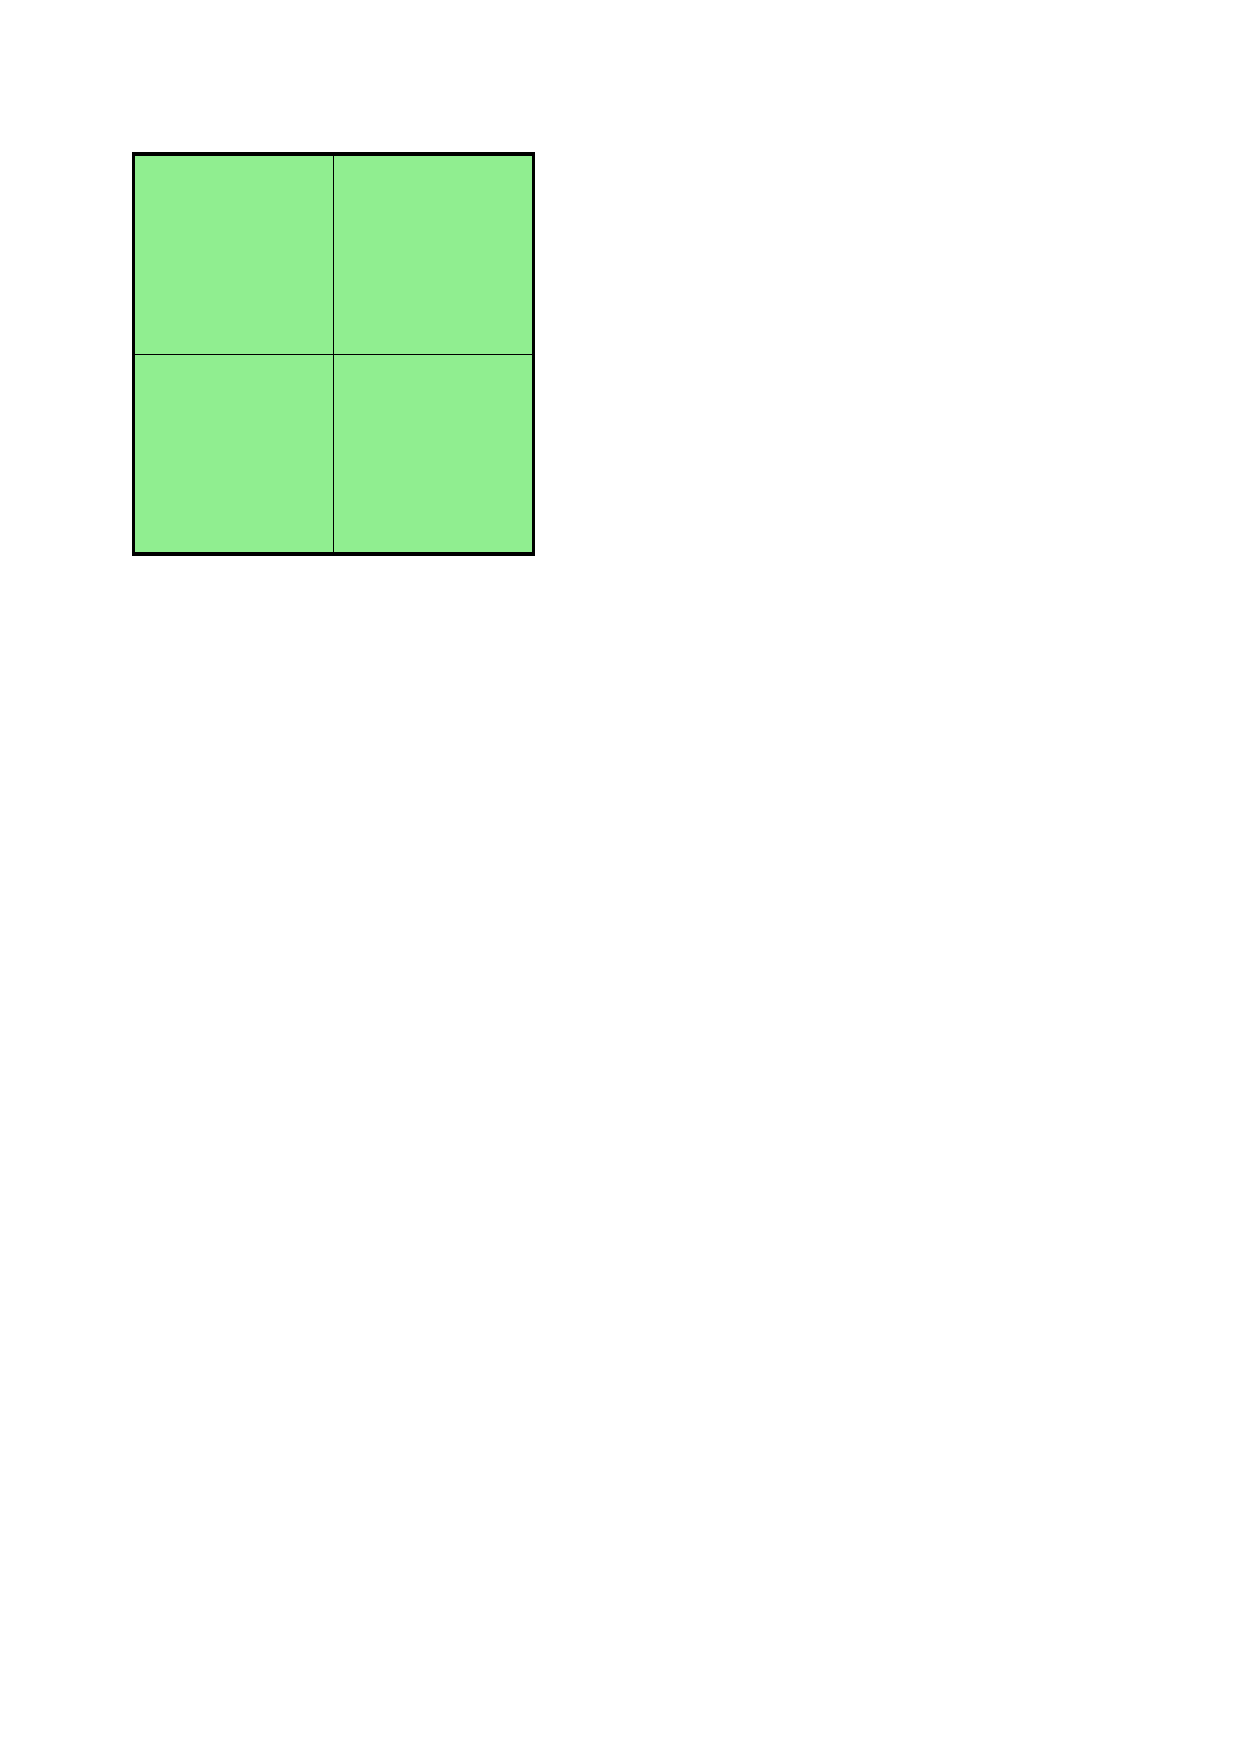
\includegraphics[scale=\normalipe]{ch01-ctverec-sobepodobnost.pdf}
        \caption{Rozdělení na čtyři menší čtverce.}
        \label{subfig:sobepodobnost-ctverce-1}
    \end{subfigure}
    \begin{subfigure}[b]{\subfigwidth}
        \centering
        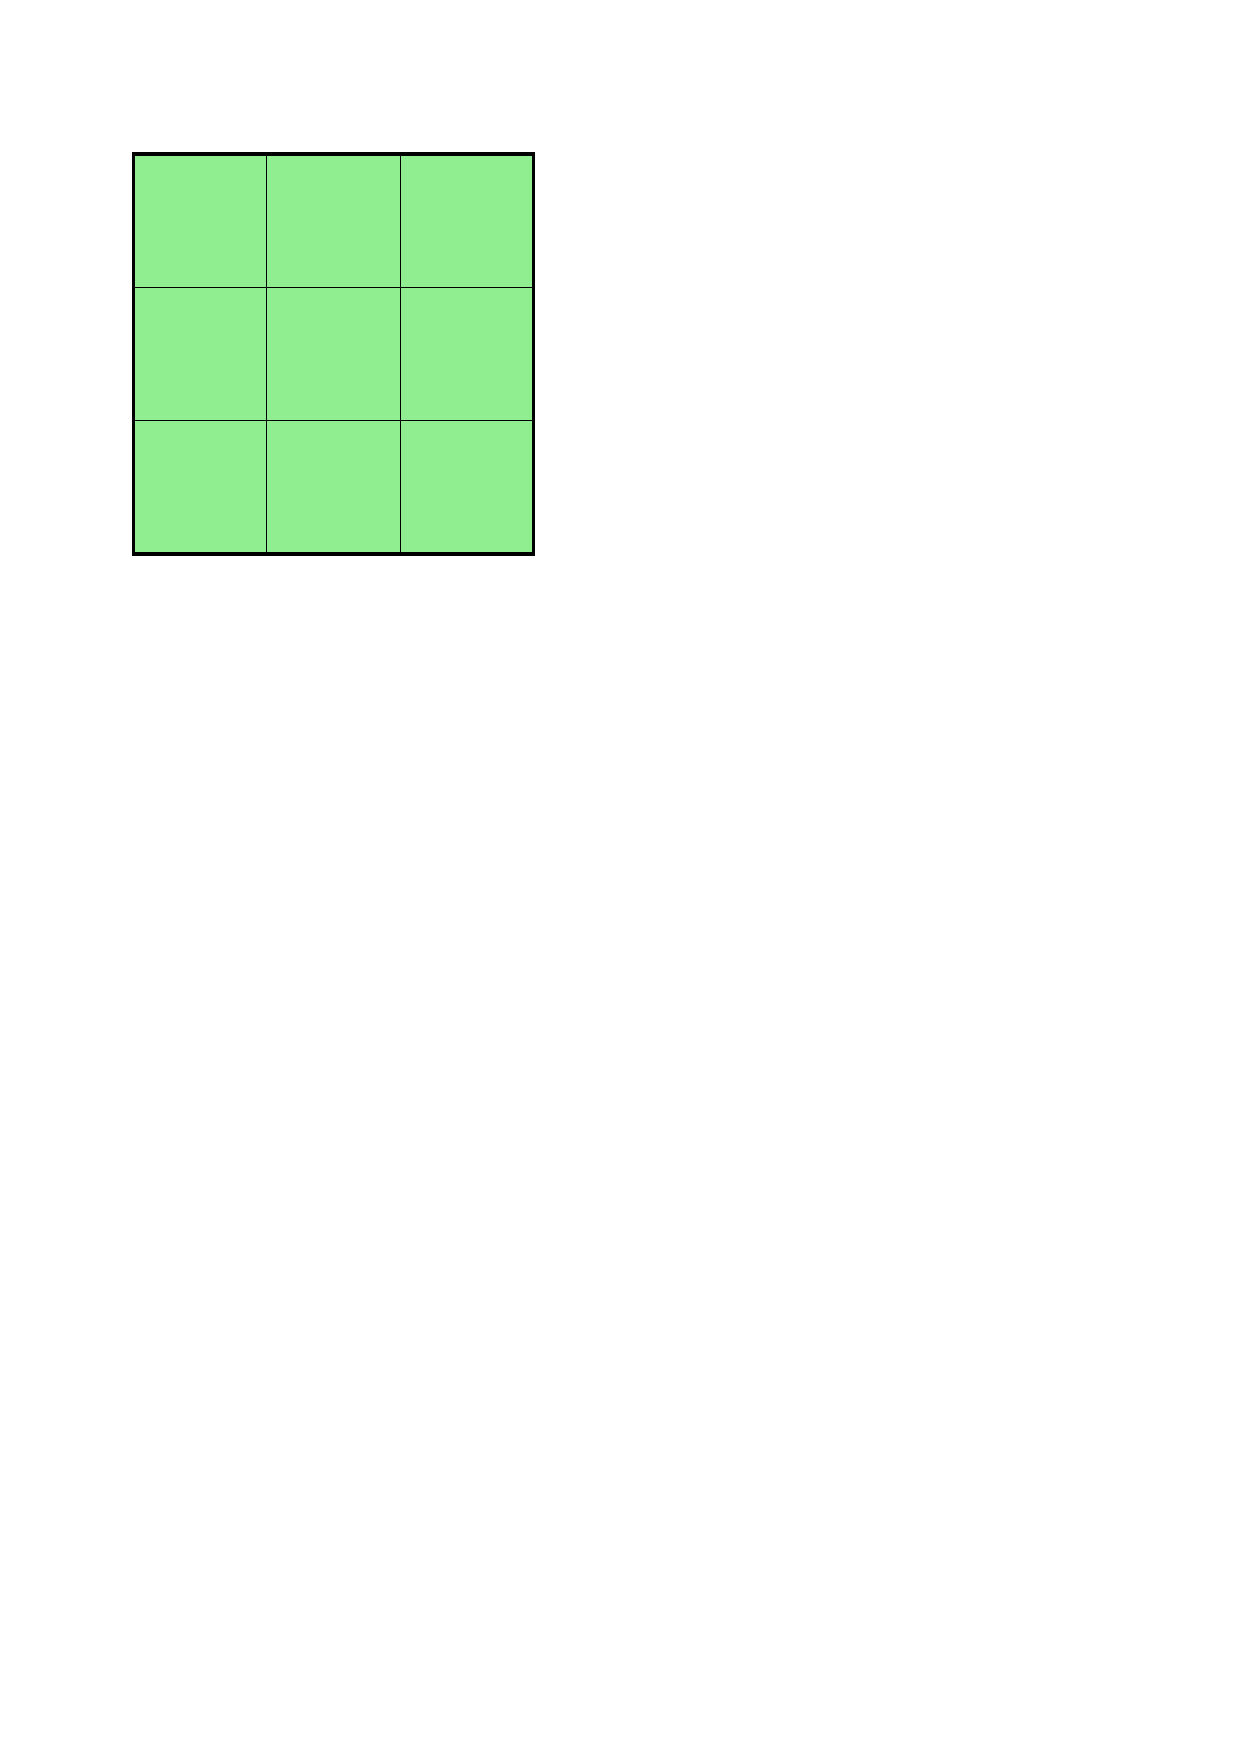
\includegraphics[scale=\normalipe]{ch01-ctverec-sobepodobnost-2.pdf}
        \caption{Jiná možnost rozdělení čtverce.}
        \label{subfig:sobepodobnost-ctverce-2}
    \end{subfigure}
    \caption{Soběpodobnost čtverce.}
    \label{fig:sobepodobnost-ctverce}
\end{figure}
Podobně např. i~obyčejná úsečka je taktéž soběpodobná,~protože ji můžeme rozdělit na $k$ stejných částí (viz obrázek~\ref*{fig:sobepodobnost-usecky}).\par
\begin{figure}[h]
    \centering
    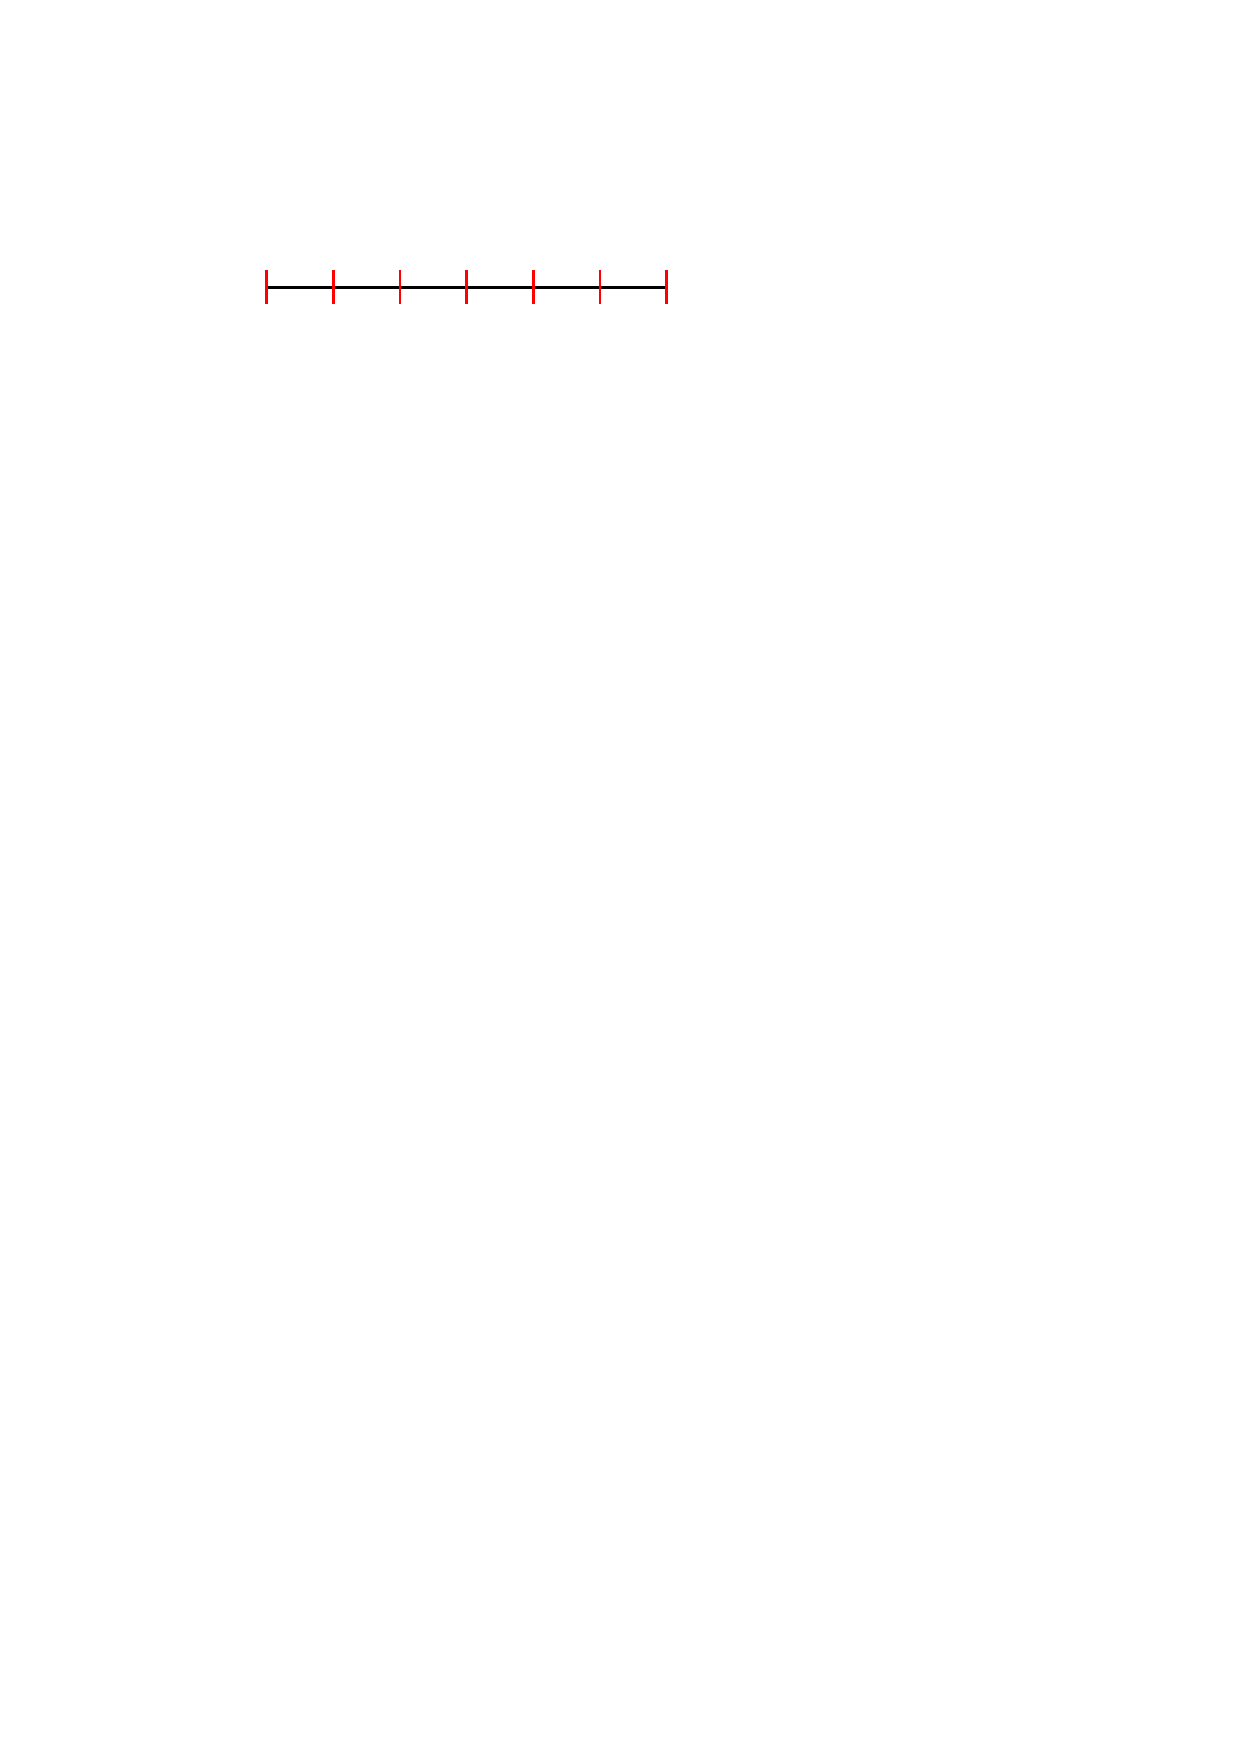
\includegraphics[scale=\normalipe]{ch01-usecka-sobepodobnost.pdf}
    \caption{Úsečka rozdělená na šest stejných částí.}
    \label{fig:sobepodobnost-usecky}
\end{figure}
K čemu nám takové uvědomění vlastně je? Zmenšíme-li úsečku $k$-krát,~pak budeme potřebovat přesně $k$ těchto částí,~abychom dostali úsečku původní délky. U~čtverce (nebo obdélníku obecně) při změnšení délky strany $k$-krát budeme potřebovat $k^2$ daných útvarů pro obdržení čtverce s~původním obsahem.\footnote{Obdélník zmenšený $k$-krát bude mít strany délek $a/k,\,b/k$,~tedy jeho obsah bude
\[\dfrac{ab}{k^2}=\dfrac{S}{k^2},\]
kde $S$ je obsah původního obdélníka.}
Pro krychli bude situace podobná,~$k$-krát zmenšená kopie bude potřeba $k^3$-krát,~abychom dostali krychli o~původním objemu (viz obrázek~\ref{fig:krychle-sobepodobnost}).
\begin{figure}[h]
    \centering
    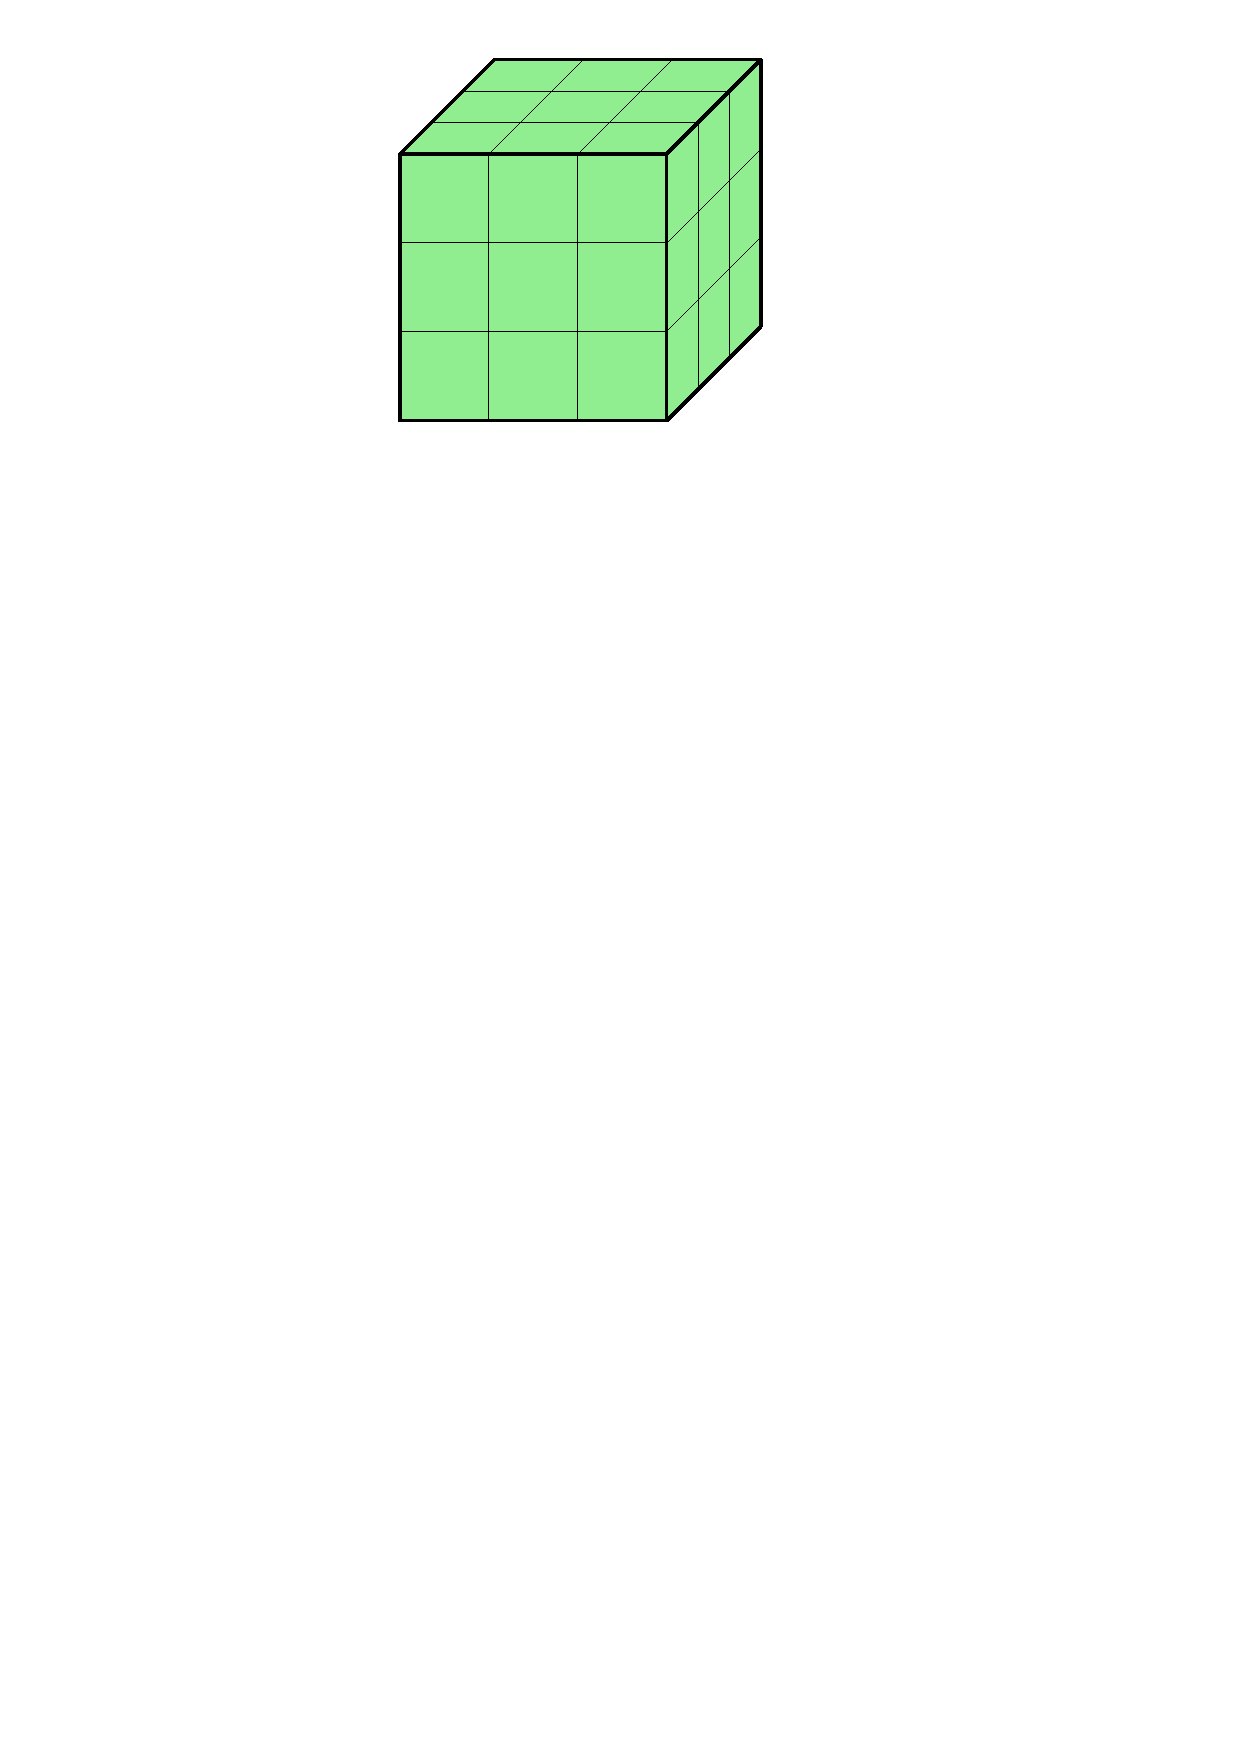
\includegraphics[scale=\normalipe]{ch01-krychle-sobepodobnost.pdf}
    \caption{Krychle rozdělená na 27 stejných částí.}
    \label{fig:krychle-sobepodobnost}
\end{figure}
Lze si všimnout,~že v~závislosti na \emph{dimenzi} objektu se mění daný exponent. Vztah lze tak zobecnit na
\begin{equation}\label{eq:pocet-utvaru}
    N(k)=k^d
\end{equation}
kde $N(k)$ je počet nových útvarů v~závislosti na faktoru $k$ a~číslu $d$. Intuitivně je nejspíše jasné,~že dimenze útvaru je takové číslo $d$,~pro které platí rovnost \eqref{eq:pocet-utvaru}.

Toto je jeden z~možných způsobů,~jak lze chápat koncept dimenze. Jednoduchou úpravou rovnosti \eqref{eq:pocet-utvaru} dostaneme
\[d=\log_k{N(k)}=\dfrac{\ln{N(k)}}{\ln{k}}.\]
(Obecně lze volit jakýkoliv přípustný základ logaritmů,~tj $d=\log_b{N(k)}/\log_b{k}$ pro $b\in\R_+\setminus\set{1}$.)

Dimenze v~tomto pojetí skutečně dává dobrý smysl. Pro "klasické" geometrické objekty vychází dimenze vždy celočíselně (viz tabulka \ref{table:eukleides-dimenze}).
\begin{table}[h]
    \centering
    \begin{tabular}{r|cc}
    Útvar    & $N(k)$ & $d=\ln{N(k)}/\ln{k}$ \\ \hline
    Úsečka   & $3$      & $1$                          \\
    Čtverec  & $9$      & $2$                          \\
    Krychle  & $27$     & $3$                          \\
    Teserakt & $81$     & $4$                          \\
    \end{tabular}
    \caption{Hodnoty dimenze $d$ pro různé útvary.}
    \label{table:eukleides-dimenze}
\end{table}

Na této myšlence je založen pojem tzv. \emph{fraktální dimenze}\index{fraktální dimenze}\index{dimenze!fraktální}. Existuje více neekvivalentních způsobů její definice. Jedna z~nich,~které se dále nyní v~této sekci budeme držet,~se v~anglicky psané literatuře nazývá \emph{"box-counting dimension"}\index{box-counting dimenze}\index{dimenze!box-counting},~odkud plyne i~značení $\dimB$. Pro útvar $F$ (formálně vzato množinu bodů) definujeme 
\begin{equation}\label{eq:fraktalni-dimenze}
    \dimB{F}=\lim_{\varepsilon\to 0_+}{\dfrac{\ln{N_\varepsilon(F)}}{\ln{\left(\frac{1}{\varepsilon}\right)}}}.
\end{equation}
(Převzato z~\cite[str. 93]{Zelinka2006} a~\cite[str. 28]{Falconer2014}.) Výraz $1/\varepsilon$ zde představuje faktor podobnosti jako původní $k$ (samotné $\varepsilon$ tak hraje roli měřítka). Číslo $N_\varepsilon(F)$ je počet soběpodobných útvarů,~na které jsme rozdělili původní útvar $F$ v měřítku $\varepsilon$. Největší rozdíl zde však představuje zkoumání "limitního chování" daného výrazu.

Nejdříve poznamenejme, pro "klasické" geometrické útvary hodnota $\dimB{F}$ vychází skutečně tak, jak jsme zvyklí. Toto si ilustrujeme na příkladech~\ref{ex:fraktalni-dimenze-usecka},~\ref{ex:fraktalni-dimenze-ctverec} a~\ref{ex:fraktalni-dimenze-trojuhelnik}.
\begin{example}[Fraktální dimenze úsečky]\label{ex:fraktalni-dimenze-usecka}
    Začněme asi nejednodušším příkladem výpočtu fraktální dimenze,~a to u~úsečky (označme $\ell$). Představme si,~že úsečku \emph{jednotkové délky} rozdělíme na $N_\varepsilon(\ell)=n$ shodných dílů. Pak měřítko libovolného dílu je
    \[\varepsilon=\dfrac{1}{n}=n^{-1}.\]
    (Zde je dobré si uvědomit,~že pro $n\to\infty$,~tedy zjemňování dělení úsečky,~platí,~že $\varepsilon\to 0_+$.) Fraktální dimenzi úsečky vypočteme z~definice jako
    \[\dimB{\ell}=\lim_{\varepsilon\to 0_+}{\dfrac{\ln{N_\varepsilon(\ell)}}{\ln{\left(\frac{1}{\varepsilon}\right)}}}=\lim_{n\to\infty}{\dfrac{\ln{n}}{\ln{n}}}=1.\]
\end{example}
\begin{example}[Fraktální dimenze čtverce]\label{ex:fraktalni-dimenze-ctverec}
    Podobně,~jako v~příkladu~\ref{ex:fraktalni-dimenze-usecka}\linebreak{}výše,~můžeme stanovit i~fraktální dimenzi čtverce (označme $S$). Uvažujme tedy čtverec o~jednotkovém obsahu,~který rozdělíme $N_\varepsilon(S)=n$ shodných útvarů. Přitom víme,~že obsah mění kvadraticky vůči délce strany. Měřítko nového čtverce tak bude
    \[\varepsilon=\sqrt{\dfrac{1}{n}}=n^{-1/2}\]
    a~fraktální dimenze vychází
    \[\dimB{S}=\lim_{n\to\infty}{\dfrac{\ln{n}}{\ln{n^{1/2}}}}=\lim_{n\to\infty}{\dfrac{\ln{n}}{\frac{1}{2}\ln{n}}}=2.\]
\end{example}
Pro krychli bude výpočet naprosto analogický (viz příklad~\ref{ex:fraktalni-dimenze-ctverec}). Obecně pro $d$-rozměrnou krychli bude její fraktální dimenze\footnote{Obdobnou úvahou dojmeme k~měřítku $\varepsilon=n^{-1/d}$.} rovna $d$.\par
Zkusme se nyní oprostit od krychle k~trochu jinému útvaru.
\begin{example}[Fraktální dimenze trojúhelníka]\label{ex:fraktalni-dimenze-trojuhelnik}
    Podívejme se,~jak to dopadne s~fraktální dimenzí \emph{obecného trojúhelníku}. Každý trojúhelník $T$ lze rozdělit na čtveřici \emph{vzájemně shodných trojúhelníků $T_1,\dots,T_4$},~které vzniknou sestrojením středních příček v~původním trojúhelníka (viz obrázek~\ref{fig:trojuhelnik-sobepodobnost}).
    \begin{figure}[h]
        \centering
        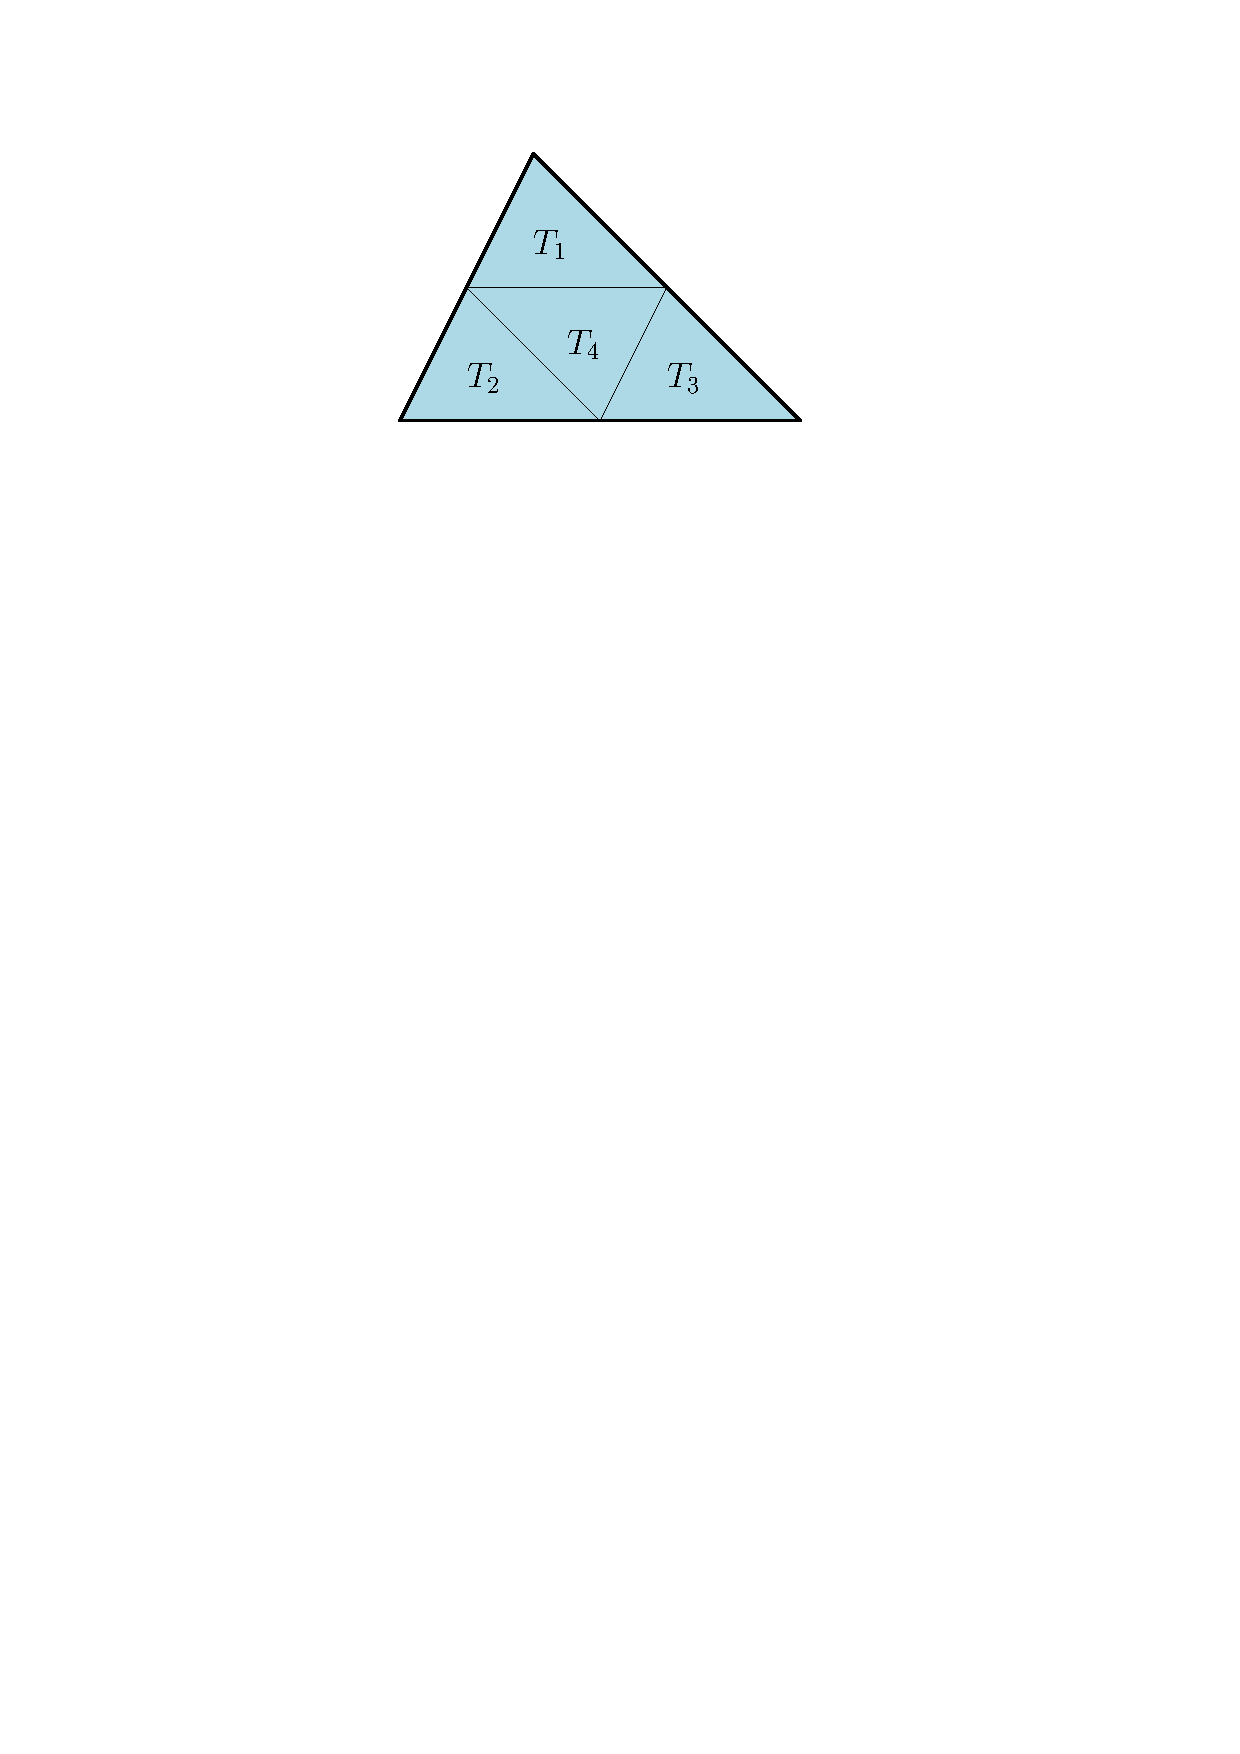
\includegraphics[scale=\normalipe]{ch01-trojuhelnik-sobepodobnost.pdf}
        \caption{Trojúhelník $T$ rozdělený na trojúhelníky $T_1,\dots,T_4$.}
        \label{fig:trojuhelnik-sobepodobnost}
    \end{figure}
    Délka každé střední příčky odpovídá polovině délky strany,~s~níž je rovnoběžná,~tedy obsah každého z~menších trojúhelníků je \emph{čtvrtina obsahu původního} trojúhelníka $T$. Tento postup můžeme opakovat pro každý z menších trojúhelníků, čímž dostaneme $4^2$ trojúhelníků. Takto můžeme postupovat libovolně dlouho,~přičemž po $n$ krocích bude počet\footnote{Výpočet bychom mohli i~zde provést ve stejném duchu jako u~úsečky,~čtverce nebo krychle. Počet částí,~na než rozdělíme trojúhelník,~označíme $N_\varepsilon(T)=n$,~přičemž měřítko pak bude $\varepsilon=n^{-1/2}$.} vzniklých trojúhelníků $N_\varepsilon(T)=4^n$,~přičemž měřítko každého z~nich bude $\varepsilon=(1/2)^n$. Fraktální dimenze tak vychází:
    \[\dimB{T}=\lim_{n\to\infty}{\dfrac{\ln{4^n}}{\ln{2^n}}}=\lim_{n\to\infty}{\dfrac{2n\ln{2}}{n\ln{2}}}=2.\]
\end{example}
Pro jednoduché útvary vychází dimenze tak,~jak bychom mohli očekávat. K~zajímavějším výsledkům však dospějeme u~fraktálů,~na něž se blíže podíváme v~následující podsekci~\ref{subsec:dimenze-fraktalu}.

\subsection{Dimenze fraktálů}\label{subsec:dimenze-fraktalu}

Co kdybychom však zkusili podobnou myšlenku aplikovat i~na \emph{fraktální objekty} jako např. Kochovu křivku, Kochovu vločku, Sierpińského trojúhelník nebo Cantorovo diskontinuum? Zkusme to. Pro připomenutí jednotlivých křivek a~výsledků k~nim si dovoluji čtenáře opětovně odkázat na sekci~\ref{sec:sobepodobnost},~kde jsou podrobněji rozebrány.

V tomto případě uvidíme,~že dochází na první pohled k~docela zvláštnímu jevu. Fraktální dimenze již totiž nemusí vycházet celočíselně,~jak jsme zvyklí.
\begin{itemize}
    \item \textbf{Kochova křivka $F_{KC}$.} V~každé iteraci nahrazujeme každou úsečku čtyřmi novými. Kompletní Kochova křivka tak obsahuje právě \emph{čtyři} kopie sebe sama zmenšené na třetinu,~tj. v~$n$-té iteraci je $N_\varepsilon(F_{KC})=4^n$,~jak jsme již odvodili (viz podsekce~\ref{subsec:kochova_krivka}).\footnote{Lze však zvolit i~jiné dělení. Např. lze na Kochovu křivku nahlížet,~že obsahuje \emph{16 kopií} sebe sama zmenšených na \emph{devítinu}.} Měřítko nově vzniklých částí je tak $\varepsilon=(1/3)^n$.
    \begin{equation}\label{eq:kochova-krivka-dimenze}
        \dimB{F_{KC}}=\lim_{\varepsilon\to 0_+}{\dfrac{\ln{N_\varepsilon(F_{KC})}}{\ln{\left(\frac{1}{\varepsilon}\right)}}}=\lim_{n\to\infty}{\dfrac{\ln{4^n}}{\ln{3^n}}}=\dfrac{\ln{4}}{\ln{3}}\approx 1{,}2618595\dots
    \end{equation}
    \item \textbf{Kochova vločka $F_{KS}$.} Začínáme s~rovnostranným trojúhelníkem o~straně délky $1$,~na jehož stranách postupně vznikne Kochova křivka. V~$n$-té iteraci je obvod Kochovy vločky $o_n$ roven $3\cdot 4^n$,~tj. i~$N_\varepsilon(F_{KS})=3\cdot 4^n$,~kde měřítko\footnote{Měřítko se ve srovnání s~Kochovou křivkou liší v~mocnině,~neboť délku nových úseků porovnáváme s~obvodem celého trojúhelníka,~nikoliv pouze délkou jedné jeho strany. Nicméně ve výpočtu bychom se mohli omezit i~jen na jednu ze stran,~výpočet by byl tak zcela identický jako u~Kochovy křivky.} nově vzniklých úseček je $\varepsilon=1/3\cdot(1/3)^n=(1/3)^{n+1}$. Není těžké se přesvědčit,~že fraktální dimenze vychází stejně,~jako u~Kochovy křivky:
    \begin{equation}\label{eq:kochova-vlocka-dimenze}
        \dimB{F_{KS}}=\lim_{n\to\infty}{\dfrac{\ln{3\cdot 4^n}}{\ln{3^{n+1}}}}=\lim_{n\to\infty}{\dfrac{\ln{4^n}\overbrace{\left(1+\frac{\ln{3}}{\ln{4^n}}\right)}^{\to 1}}{\ln{3^n}\underbrace{\left(1+\frac{\ln{3}}{\ln{3^n}}\right)}_{\to 1}}}=\dfrac{\ln{4}}{\ln{3}}
    \end{equation}
    \item \textbf{Sierpińského trojúhelník $F_{ST}$.} V~každé iteraci vynecháme prostřední trojúhelník,~čímž vznikne \emph{trojice} nových trojúhelníků s~\emph{polovičním} měřítkem. Tzn.~$N_\varepsilon(F_{ST})=3^n$ pro $\varepsilon=(1/2)^n$,~a tedy
    \begin{equation}\label{eq:sierpinskeho-trojuhelnik-dimenze}
        \dimB{F_{ST}}=\lim_{n\to\infty}{\dfrac{\ln{3^n}}{\ln{2^{n}}}}=\dfrac{\ln{3}}{\ln{2}}\approx 1{,}5849625\dots
    \end{equation}
    \item \textbf{Cantorovo diskontinuum $F_{CD}$.} Vždy vyjmeme prostřední třetinu\linebreak{}úsečky,~čímž obdržíme \emph{dvojici} úseček \emph{třetinové} délky,~tj. $N_\varepsilon(F_{CD})=2^n$ pro $\varepsilon=(1/3)^n$. Fraktální dimenze tak vychází
    \begin{equation}\label{eq:cantorovo-diskontinuum-dimenze}
        \dimB{F_{CD}}=\lim_{n\to\infty}{\dfrac{\ln{2^n}}{\ln{3^n}}}=\dfrac{\ln{2}}{\ln{3}}\approx 0{,}6309297\dots
    \end{equation}
\end{itemize}
Udělejme si nyní menší souhrn a~porovnání dosud získaných výsledků (viz tabulka~\ref{table:fraktaly-eukleides-dimenze}).
\begin{table}[h]
    \centering
    \begin{tabular}{r|ccc}
        Útvar $F$                & $\varepsilon$ & $N_\varepsilon(F)$ & $\dimB{F}$         \\ \hline
        Úsečka                   & $n^{-1}$      & $n$                & 1                  \\
        Čtverec                  & $n^{-1/2}$    & $n$                & 2                  \\
        Krychle                  & $n^{-1/3}$    & $n$                & 3                  \\
        Teserakt                 & $n^{-1/4}$    & $n$                & 4                  \\
        $d$-rozměrná krychle     & $n^{-1/d}$    & $n$                & $d$                \\
        Obecný trojúhelník       & $(1/2)^n$     & $4^n$              & 2                  \\
        Kochova křivka           & $(1/3)^n$     & $4^n$              & $1{,}2618595\dots$ \\
        Kochova vločka           & $(1/3)^{n+1}$ & $3\cdot 4^n$       & $1{,}2618595\dots$ \\
        Sierpińského trojúhelník & $(1/2)^n$     & $3^n$              & $1{,}5849625\dots$ \\
        Cantorovo diskontinuum   & $(1/3)^n$     & $2^n$              & $0{,}6309297\dots$ \\
    \end{tabular}
    \caption{Porovnání fraktálních dimenzí $d_k$ různých objektů.}
    \label{table:fraktaly-eukleides-dimenze}
\end{table}
Můžeme si všimnout,~že zatímco u~"klasických" objektů vychází fraktální dimenze \emph{celočíselná},~u~(zmíněných) fraktálů vychází \emph{neceločíselně},~ba dokonce i~iracionálně.

\subsection{Topologická dimenze}\label{subsec:topologicka-dimenze}

Výsledky z~předešlé části~\ref{subsec:dimenze-fraktalu} se můžou zdát poněkud překvapující. Jak je vůbec možné,~že dimenze nemusí vycházet nutně celočíselná? Ač se to možná zdá jako nesmyslný výsledek,~je třeba si uvědomit,~jak vlastně koncept dimenze chápeme. Na jednu stranu na ni lze nahlížet jako na mocninu "s níž se zvyšuje" obsah/objem tělesa, měníme-li měřítko. Naopak čtenář znalý lineární algebry si možná vzpomene,~že v~této matematické disciplíně se na dimenzi nahlíží jako na \emph{mohutnost libovolné báze daného vektorového prostoru},~která naopak vychází vždy pouze celočíselně, případně nekonečná,~avšak nelze s~ní dobře zachytit hlubší detail geometrie u~objektů,~jako jsou právě fraktály.

Dalším možným pojetím pojmu dimenze nám dává tzv. \emph{topologická dimenze}\index{dimenze!topologická}\index{topologická dimenze}. Ty totiž daleko více odpovídají našemu intuitivnímu chápání tohoto pojmu,~neboť se vždy jedná o~celé číslo,~jak ho známe ze školní geometrie. Existuje více topologických dimenzí\footnote{Jiným příkladem takové dimenze je \emph{induktivní dimenze}.},~které si,~co do definice,~obecně nejsou ekvivalentní,~ačkoliv ve většině standardních případů splývají. My se zde pro ilustraci podíváme na tzv. \emph{Lebesgueovu pokrývací dimenzi}\index{dimenze!Lebesgueova pokrývací}\index{Lebesgueova pokrývací dimenze} (dále jen již "topologickou dimenzi") pojmenovanou po francouzském matematikovi \name{Henri Lebesgueovi}\index{Henri Lebesgue} (1875--1941). Myšlenka definice je založena na pokrývání objektu (formálně vzato \emph{množiny bodů}) tzv. \emph{otevřenými množinami}\index{množina!otevřená}\index{otevřená množina}.\footnote{Otevřená množina je zobecnění pojmu otevřeného intervalu reálných čísel. Neformálně řečeno je to taková množina $X$,~kde pro každý její bod $x\in X$ patří do této množiny i~nějaké $\varepsilon$-okolí tohoto bodu (patří do ní i~body,~které jsou "dostatečně blízko").} Formální definici si zde v~rámci zachování jednoduchosti odpustíme,~avšak pro hlubší matematický základ si dovolím čtenáře odkázat např. na knihu \cite{Engelking1989}. Avšak pokusíme se ji alespoň nastínit.

Množina $X$ má topologickou dimenzi $\dimL{X}=n$,~pokud $n$ je nejmenší číslo,~takové,~že pro každé pokrytí otevřenými množinami\footnote{Formálněji to znamená,~že $A_1,\dots,A_n$ jsou otevřené množiny,~takové,~že platí $X\subseteq\bigcup_{i=1}^n{A_i}$.} $\mathcal{U}$ existuje zjemnění\footnote{Zjemněním pokrytí $\mathcal{U}$ nazýváme takové pokrytí $\mathcal{U}^\prime$ množiny $X$,~kde každá množina $A_i^\prime\in\mathcal{U}^\prime$ je \emph{podmnožinou} nějaké množiny $A_j$ původního pokrytí $\mathcal{U}$.}\index{zjemnění} $\mathcal{U}^\prime$ takové,~že každý bod $x\in X$ náleží nejvýše $n+1$ množin pokrytí $\mathcal{U}$.

% Obecně množina $X$ má topologickou dimenzi $\dimL{X}=n$,~pokud danou množinu nelze pokrýt\footnote{Formálněji to znamená,~že $A_1,\dots,A_n$ jsou otevřené množiny,~takové,~že platí $X\subseteq\bigcup_{i=1}^n{A_i}$.} lib. otevřenými množinami,~tak,~že pro každé zjemnění $\mathcal{U}$ tohoto pokrytí platí,~že každý jeho bod $x$ je obsažen v~průniku nejvýše $n+1$ množin $\mathcal{U}$.

Tuto ideu si zkusíme přiblížit na příkladu topologické dimenze úsečky (viz obrázek~\ref{fig:usecka-zjemneni}).
\begin{figure}[h]
    \centering
    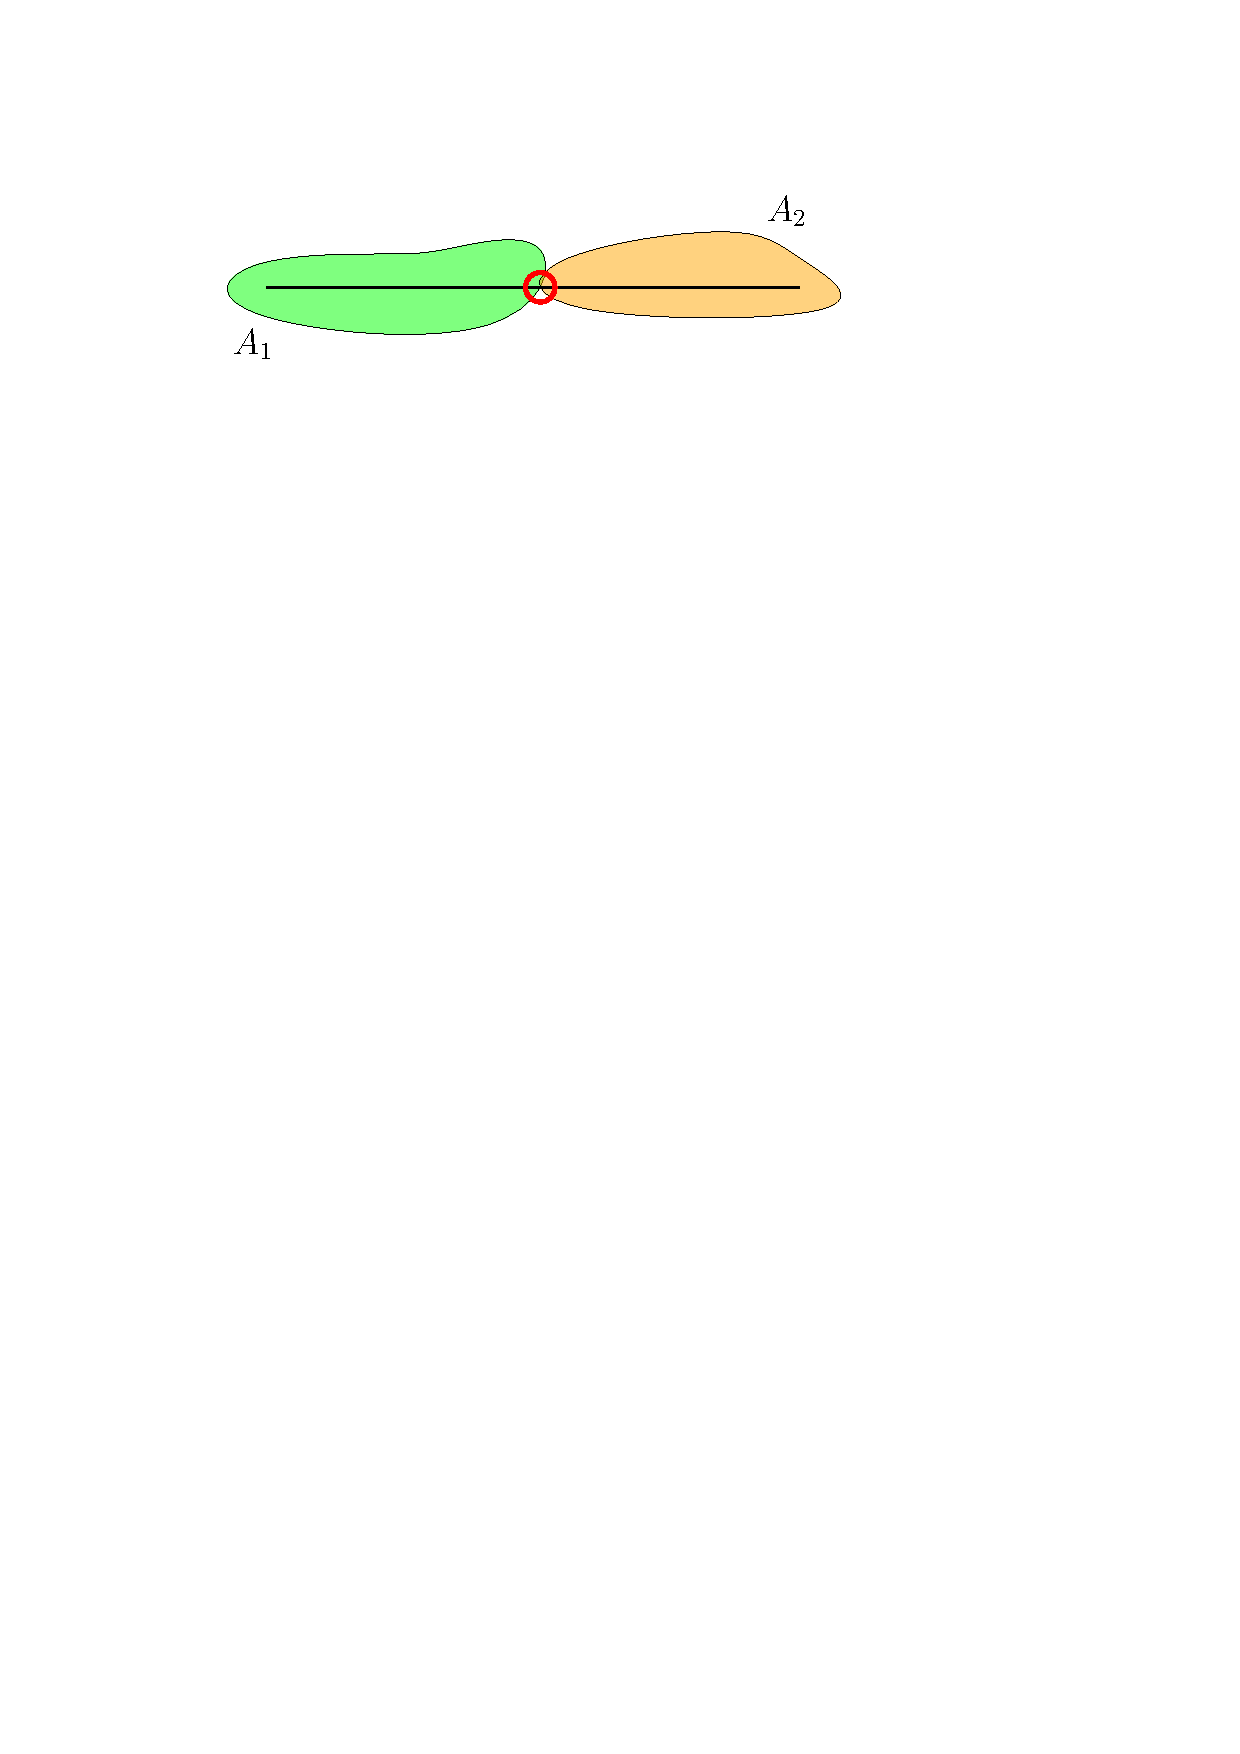
\includegraphics[scale=\normalipe]{ch01-usecka-pokryti-1.pdf}\\\qquad\\
    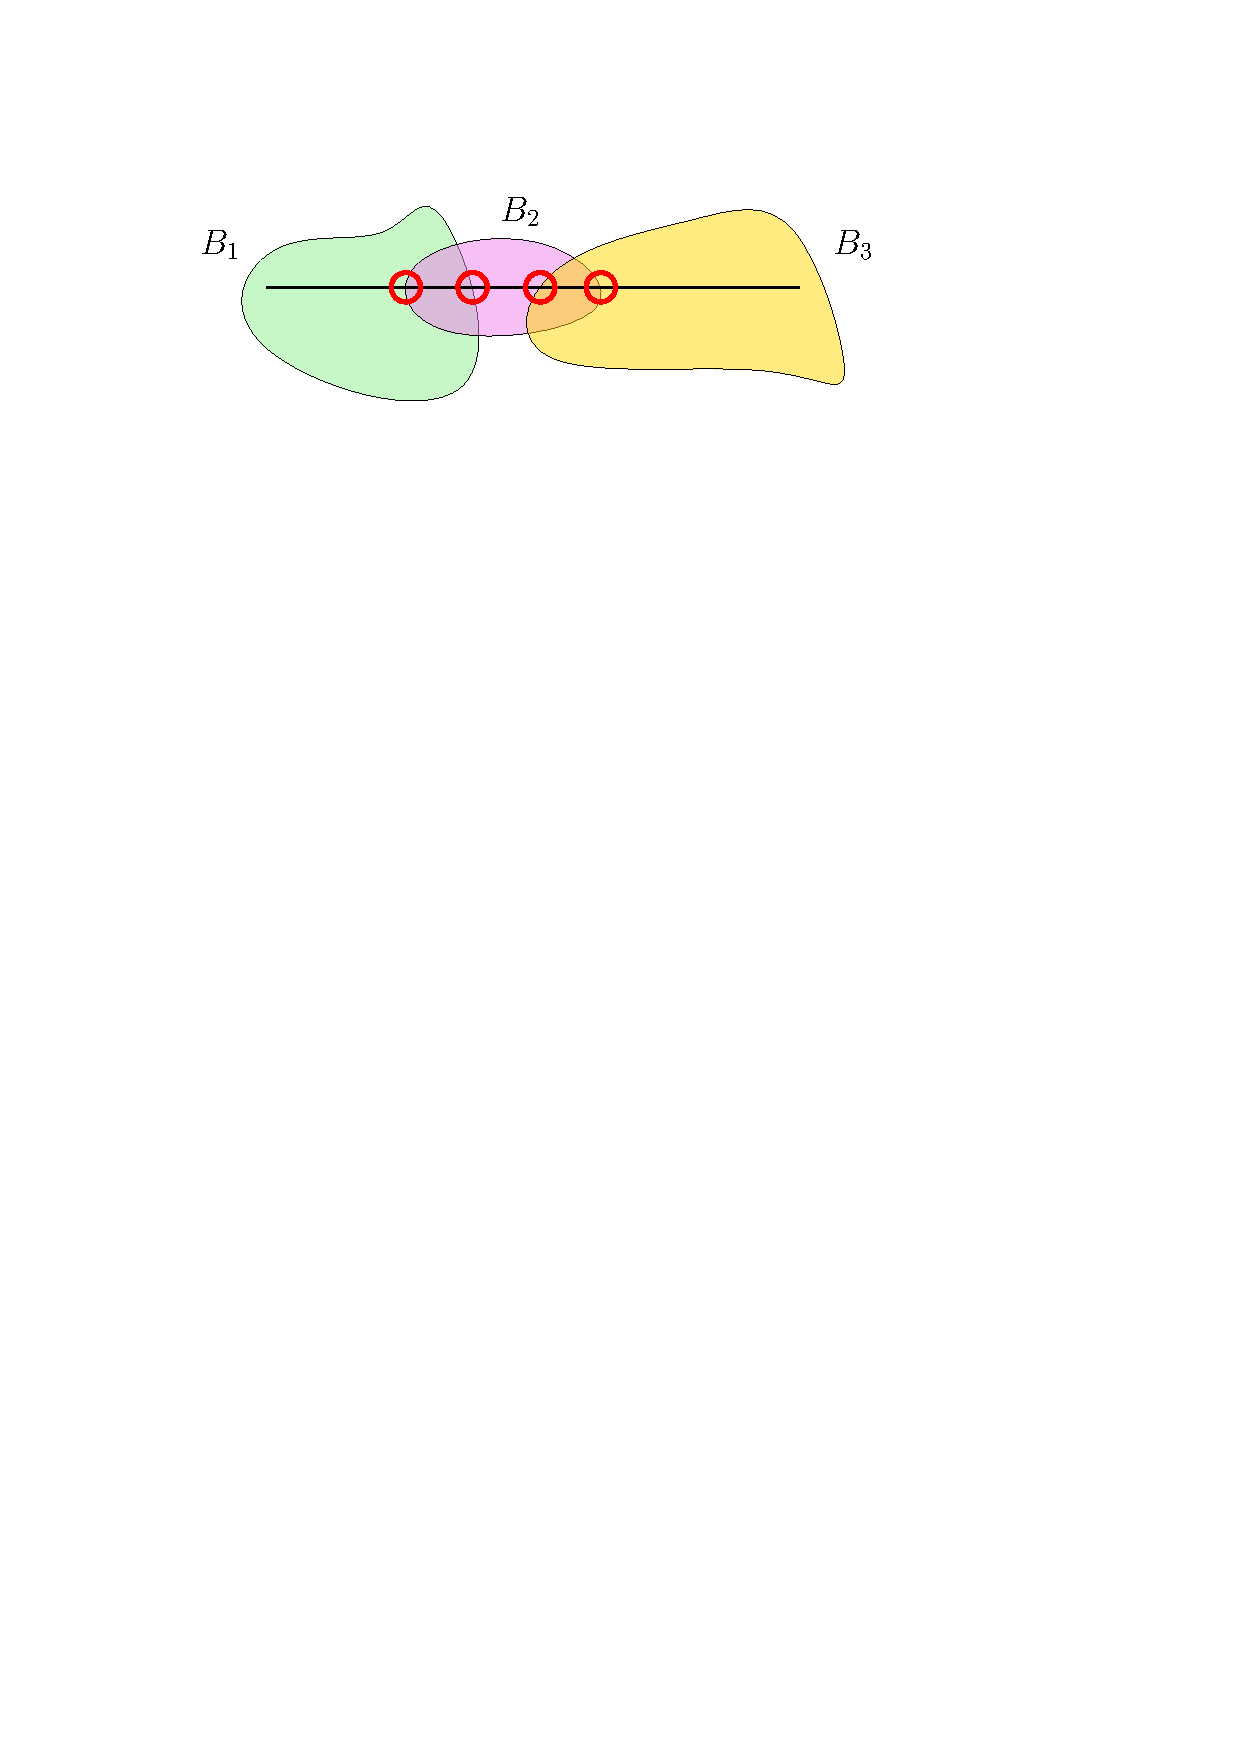
\includegraphics[scale=\normalipe]{ch01-usecka-pokryti-2.pdf}\\\qquad\\
    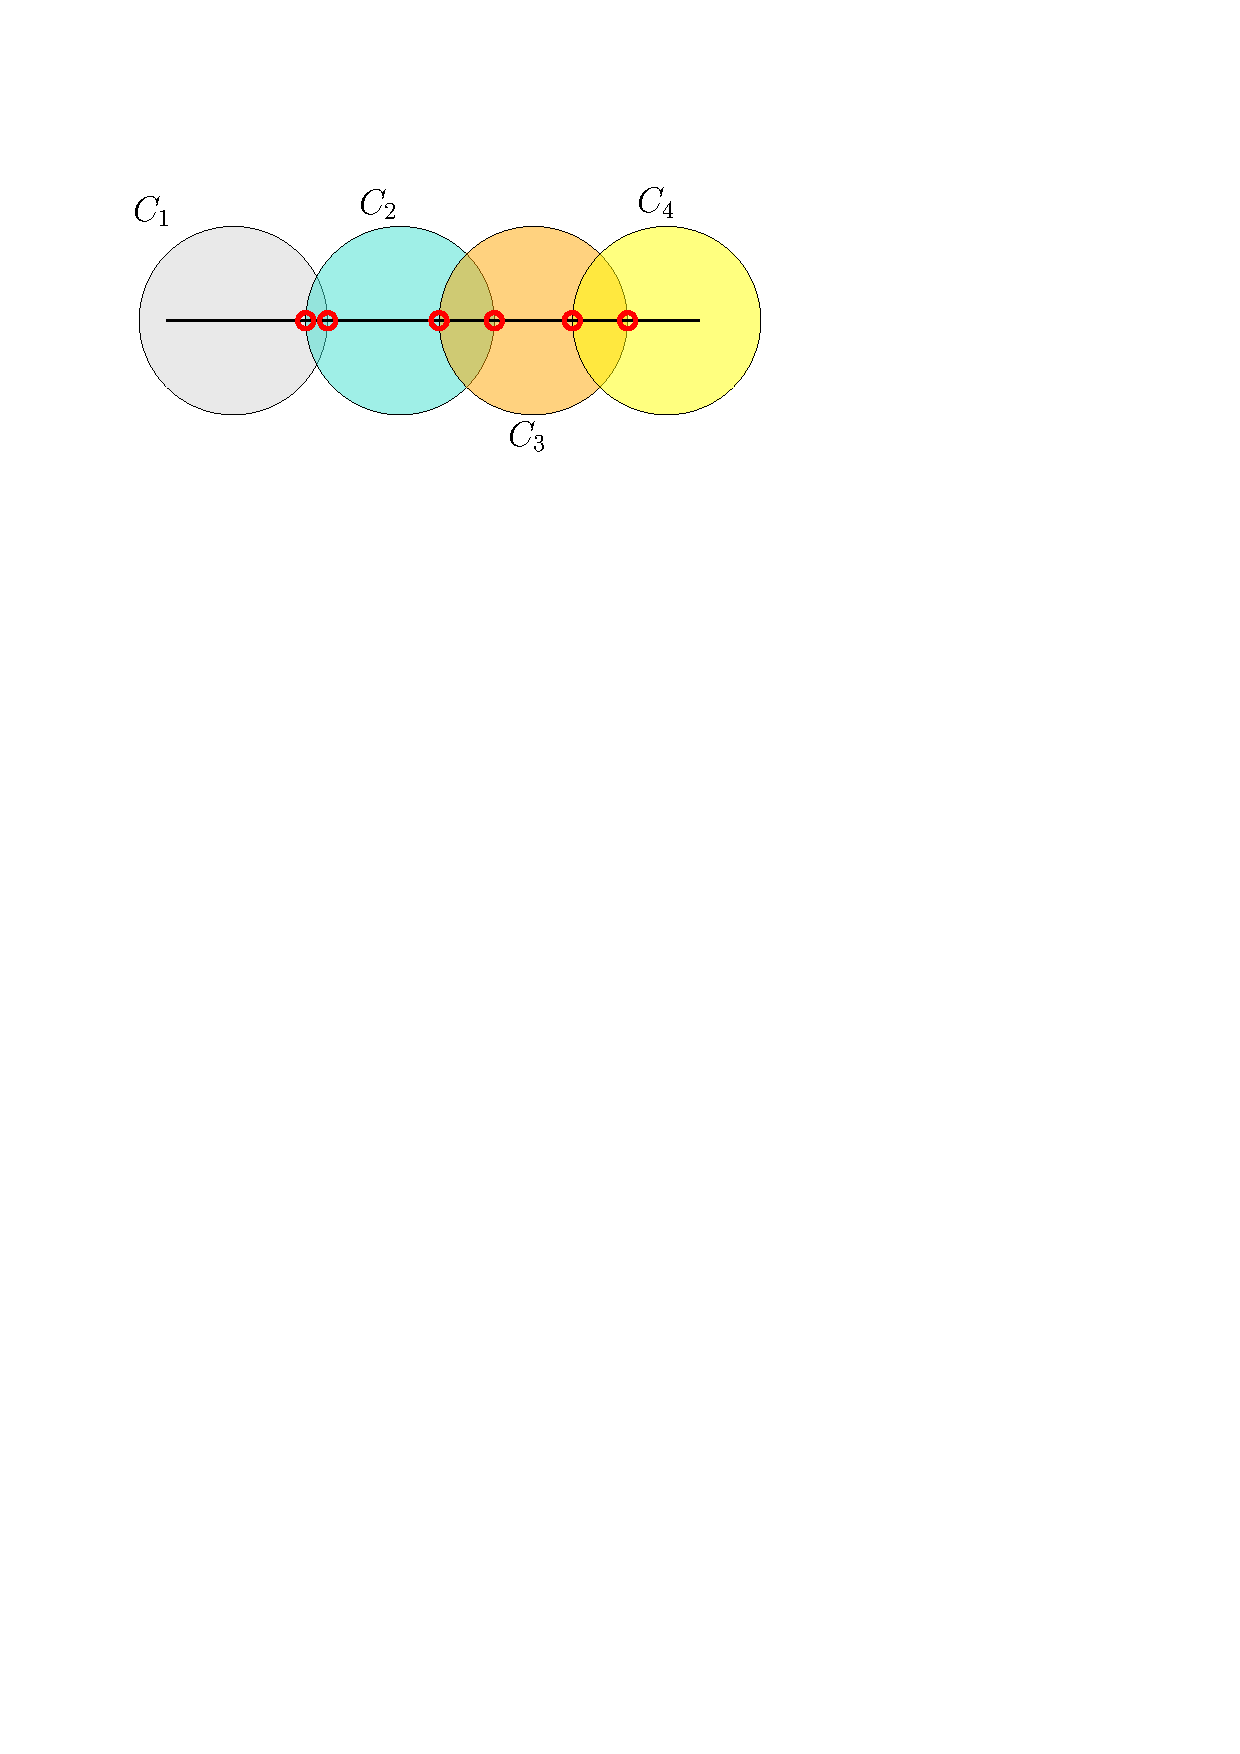
\includegraphics[scale=\normalipe]{ch01-usecka-pokryti-3.pdf}\\\qquad\\
    \caption{Různé možnosti (pod)pokrytí úsečky.}
    \label{fig:usecka-zjemneni}
\end{figure}
Pro libovolné pokrytí lze ukázat,~že každý bod je obsažen maximálně ve \emph{dvou množinách} vhodně zvoleného zjemnění,~tedy topologická dimenze úsečky je $1$. Podobně např. pro čtverec lze dojít k~závěru,~že pro každé pokrytí existuje zjemnění takové,~že každý bod obsažen maximálně ve \emph{třech množinách},~tedy jeho topologická dimenze je 2,~jak bychom očekávali (viz obrázek~\ref{fig:ctverec-zjemneni}).
\begin{figure}[h]
    \centering
    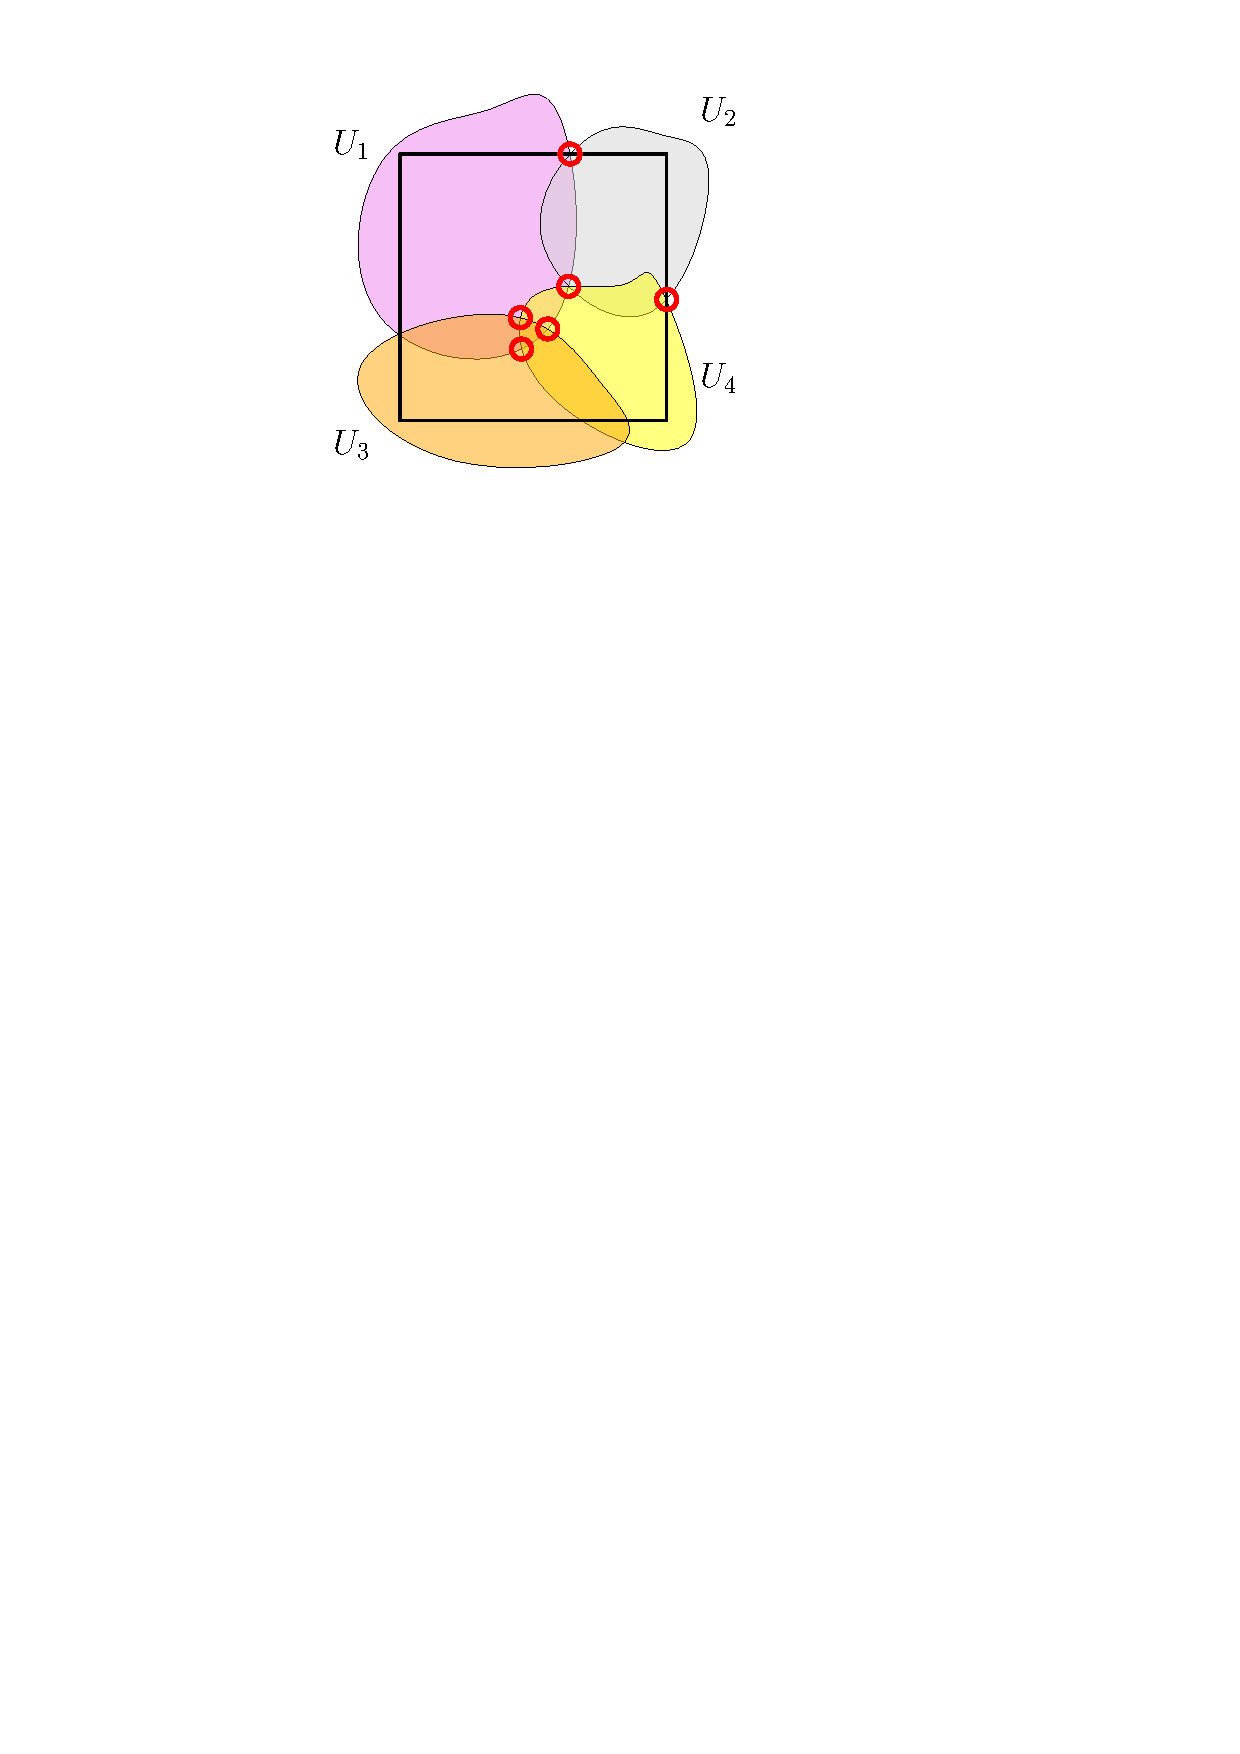
\includegraphics[scale=\normalipe]{ch01-ctverec-pokryti.pdf}
    \caption{Možné (pod)pokrytí čtverce.}
    \label{fig:ctverec-zjemneni}
\end{figure}
Porovnejme nyní topologickou dimenzi vůči dimenzi fraktální. Jak jsme se již přesvědčili v~příkladech~\ref{ex:fraktalni-dimenze-usecka},~\ref{ex:fraktalni-dimenze-ctverec} a~\ref{ex:fraktalni-dimenze-trojuhelnik},~pro "standardní" útvary je fraktální dimenze celočíselná (ač jsou i~další,~které jsme neuvedli),~zatímco v~podsekci~\ref{subsec:dimenze-fraktalu} jsme zjistili,~že u~fraktální dimenze fraktálů tomu tak být nemusí. Přitom však topologická dimenze fraktálních útvarů je (a dokonce musí být) celočíselná (viz tabulka~\ref{table:fraktalni-topologicka-dimenze}).
\begin{table}[h]
    \centering
    \begin{tabular}{r|cc}
    Útvar $F$                & $\dimB{F}$            & $\dimL{F}$ \\\hline
    Úsečka                   & 1                     & 1          \\
    Čtverec                  & 2                     & 2          \\
    Krychle                  & 3                     & 3          \\
    Teserakt                 & 4                     & 4          \\
    $d$-rozměrná krychle     & $d$                   & $d$        \\
    Kochova křivka           & $1{,}2618595\dots$    & 1          \\
    Kochova vločka           & $1{,}2618595\dots$    & 1          \\
    Sierpińského trojúhelník & $1{,}5849625\dots$    & 2          \\
    Cantorovo diskontinuum   & $0{,}6309297\dots$    & 0      
    \end{tabular}
    \caption{Porovnání fraktální a~topologické dimenze útvarů.}
    \label{table:fraktalni-topologicka-dimenze}
\end{table}
Fraktální dimenze tak oproti té topologické daleko lépe zachycuje informaci o~detailní geometrii daných objektů.
\section{Co je to fraktál?}\label{sec:co-je-to-fraktal}
\emph{Tak co je to tedy ten "fraktál"?}\index{fraktál} Odpovědi na tuto otázku jsme se poměrně dlouhou dobu vyhýbali a~onen termín,~popř. jeho přídavnou variantu \emph{"fraktální"},~jsme používali čistě na intuitivní úrovni. Ač jsme se zatím obešli bez jeho formálnějšího upřesnění,~bylo by možná při nejmenším slušné se o~to alespoň pokusit. V~předešlé sekci~\ref{sec:fraktalni_dimenze} jsme pokryli \emph{fraktální} a~\emph{topologickou dimenzi},~které jsme následně použili na příkladech konkrétních útvarů (konkrétně viz tabulky~\ref{table:fraktaly-eukleides-dimenze} a~\ref{table:fraktalni-topologicka-dimenze}).

Již jsme si všimli,~že u~fraktálních útvarů vychází fraktální dimenze $\dimH$ neceločíselně oproti jejich topologické dimenzi $\dimL$,~která je vždy celočíselná. To by se mohlo zdát jako dobrá charakteristika fraktálů. Avšak existují útvary,~jejichž fraktální a~topologická dimenze se shodují,~přestože také mají "fraktální charakter". Pro příklad nemusíme chodit nikterak daleko,~pravděpodobně nejznáměnším útvarem je v~tomto ohledu \emph{Mandelbrotova množina}\index{množina!Mandelbrotova}\index{Mandelbrotova mnozina},~jejiž fraktální i~topologická dimenze je rovna $2$ (blíže se na ni podíváme v~podsekci~\ref{subsec:mandebrotova-mnozina}). Jiná definice zase naopak popisuje fraktál jako útvar,~jehož Hausdorffova dimenze (na tu se blíže podíváme v~sekci~\ref{sec:hausdorffova-mira-dimenze}) je ostře větší než dimenze topologická. Problém (a také důvod,~proč jsme definici toho pojmu vyhývali) je však zkrátka ten,~že dodnes \textbf{není známá} žádná univerzální definice fraktálu. \cite[str. 226]{Voracova2022}

Je to možná lehce zklamávající,~nicméně dobrou zprávou je,~že ani pro další výklad ona absence formální definice fraktálu nebude překážkou. V~dalším textu se zaměříme (mj.) především na jejich klasifikaci (viz kapitola~\ref{chapter:klasifikace-fraktalu}) a~další vlastnosti.